% This LaTeX document needs to be compiled with XeLaTeX.
\documentclass[10pt]{article}
\usepackage[utf8]{inputenc}
\usepackage{amsmath}
\usepackage{amsfonts}
\usepackage{amssymb}
\usepackage[version=4]{mhchem}
\usepackage{stmaryrd}
\usepackage{hyperref}
\hypersetup{colorlinks=true, linkcolor=blue, filecolor=magenta, urlcolor=cyan,}
\urlstyle{same}
\usepackage{caption}
\usepackage{graphicx}
\usepackage[export]{adjustbox}
\graphicspath{ {./images/} }
\usepackage{multirow}
\usepackage{diagbox}
\usepackage[fallback]{xeCJK}
\usepackage{polyglossia}
\usepackage{fontspec}
\usepackage{newunicodechar}
\IfFontExistsTF{Noto Serif CJK JP}
{\setCJKmainfont{Noto Serif CJK JP}}
{\IfFontExistsTF{STSong}
  {\setCJKmainfont{STSong}}
  {\IfFontExistsTF{Droid Sans Fallback}
    {\setCJKmainfont{Droid Sans Fallback}}
    {\setCJKmainfont{SimSun}}
}}

\setmainlanguage{italian}
\IfFontExistsTF{CMU Serif}
{\setmainfont{CMU Serif}}
{\IfFontExistsTF{DejaVu Sans}
  {\setmainfont{DejaVu Sans}}
  {\setmainfont{Georgia}}
}

\title{$\sqrt{1} 70+$ }

\author{}
\date{}


\newunicodechar{□}{\ifmmode\square\else{$\square$}\fi}
\newunicodechar{✓}{\ifmmode\checkmark\else{$\checkmark$}\fi}

\begin{document}
\maketitle
\captionsetup{singlelinecheck=false}
\section{WNET+}
Manuale dell' utente\\
Diode Laser con Android System

Capitolo 1 Istruzioni per l'utente\\
1.1 Sicurezza\\
1.2 Formazione degli operatori\\
1.3 Sicurezza degli impianti elettrici e delle apparecchiature

Capitolo 2 Introduzione del prodotto\\
2.1 Descrizione del prodotto\\
2.2 Struttura e prestazioni del prodotto\\
2.2.1 Composizione strutturale\\
2.2.2 Specifiche delle apparecchiature

\section{W $/ \sqrt{6}+$}
2.3 Applicazioni di trattamento\\
2.4 Accessori per apparecchiature

CAPITOLO 3 INSTALLAZIONE\\
3.1 Processo di installazione delle apparecchiature\\
3.2 Requisiti di installazione e quantità di acqua immessa\\
3.2.1 Direttiva sulle acque di scarico\\
3.2.2 Prove del ciclo dell'acqua\\
3.2.2 Installazione delle maniglie di movimentazione

Capitolo 4 Insegnamento del software\\
4.1 Display funzionante\\
4.1.1 Descrizione del display funzionante\\
4.1.2 Istruzioni di allarme\\
4.2 Visualizzazione delle impostazioni di sistema\\
4.2.1 Istruzioni per la visualizzazione delle impostazioni di sistema\\
4.2.2 Impostazioni dei parametri in background\\
4.3 Istruzioni per l'uso del software\\
4.4 Modalità di funzionamento del dispositivo\\
4.5 Precauzioni dopo il trattamento

Capitolo 5 Manutenzione\\
5.1 Pulizia delle attrezzature\\
5.2 Pulizia e sostituzione delle maniglie di movimentazione\\
5.3 Gestione dei guasti del sistema

Capitolo 6 DISPOSIZIONI\\
Capitolo 7 protocolli medi Specifiche\\
Capitolo 8 protocolli fotobiostimolazione\\
Garanzia\\
Consenso informato\\
Certificazione

Capitolo 1 Istruzioni per l'utente\\
Si prega di leggere attentamente il manuale prima dell'operazione! Assicurarsi che l'apparecchiatura sia in condizioni di lavoro. Evita danni inutili. Se l'operatore desidera collegare il dispositivo ad altre periferiche, leggere attentamente il manuale delle periferiche.

\subsection{Sicurezza}
Il dispositivo ha una funzione di autotest. Quando il dispositivo è acceso, il processore di sistema eseguirà un autotest. Inoltre, il processore di sistema eseguirà un autotest continuo e distanziato durante il funzionamento dell'apparecchiatura.

In caso di emergenza, premere il pulsante di emergenza (pulsante rosso) per spegnere il dispositivo.

Nota: Solo personale addestrato dal rivenditore ha il diritto di mantenere le strutture interne dello strumento e qualsiasi trattamento non autorizzato può causare danni allo strumento e invalidare la garanzia.

\subsection{Formazione degli operatori}
Il dispositivo può essere utilizzato solo da persone che hanno una formazione professionale per comprendere gli effetti terapeutici e i possibili rischi. L'operatore deve leggere attentamente il manuale dell'utente prima di utilizzare l'apparecchiatura. Nel corso del trattamento, la sala di trattamento deve essere contrassegnata con le parole "non è consentito l'ingresso di persone non correlate". Prima dell'intervento, l'operatore deve informare il paziente dei possibili rischi del trattamento e il paziente deve raggiungere un accordo scritto sul trattamento. Il successo del trattamento dipende principalmente dall'esperienza e dalla competenza dell'operatore. Durante il trattamento, l'operatore deve indossare occhiali protettivi e l'oggetto del trattamento deve indossare occhiali protettivi. Gli occhiali protettivi e gli occhiali protettivi sono appositamente attrezzati dalla società di strumenti. Non indossare occhiali protettivi che non soddisfano i requisiti di sicurezza.\\
1.3 Sicurezza degli impianti elettrici e delle apparecchiature

L'alimentatore utilizzato nell'apparecchiatura è $200 \mathrm{~V} \sim 240 \mathrm{~V}(50 / 60 \mathrm{~Hz})$ dello standard internazionale per l'alimentazione monofase ( $120 \mathrm{~V} \sim 260 \mathrm{~V}, 50 / 60 \mathrm{~Hz}$ ); Presa a tre fili monofase 20 A ( $90 \sim 130 \mathrm{~V}, 50 / 60 \mathrm{~Hz}$ ). L'apparecchiatura è a contatto con il suolo attraverso tre fili e deve essere messa a terra in modo affidabile. Solo il personale autorizzato può riparare l'attrezzatura, altrimenti il periodo di garanzia scadrà.

Nota: evitare l'uso di sostanze infiammabili come acetone e alcool nell'area operativa. Quando si disinfetta l'apparecchiatura con prodotti alcolici, assicurarsi che l'alcool sia completamente evaporato prima di utilizzare l'apparecchiatura.

\section{Capitolo 2 Presentazione del prodotto}
\subsection{Descrizione del prodotto}
Il sistema Android SmartDepi è un dispositivo di depilazione laser a semiconduttore. È un dispositivo che utilizza un laser a semiconduttore continuo ad alta energia per realizzare la conversione di elettricità, luce e calore e completare il trattamento delle malattie. È una raccolta di tecnologia laser, elettronica e informatica.

Un prodotto per il trattamento laser che combina chirurgia e tecnologia \href{http://medica.Il}{medica.Il} principio di funzionamento del dispositivo di depilazione: il microprocessore controlla l'alimentazione del laser per fornire corrente costante regolabile per il modulo laser.. . Il diodo laser ad alta potenza all'interno del modulo converte l'energia elettrica in energia luminosa, la lunghezza d'onda di uscita è $755 \mathrm{~nm}+808 \mathrm{~nm}+1064 \mathrm{~nm}$, laser continuo, il raggio laser irradia il tessuto da depilare attraverso i cristalli di guida della luce, attraverso la superficie della pelle fino al follicolo pilifero, l'energia della luce viene assorbita in energia termica che distrugge il tessuto follicolo pilifero, causando la caduta dei capelli, la perdita della capacità di rigenerazione, per ottenere una depilazione permanente.

E composto principalmente da un host, un modulo di controllo e una maniglia terapeutica. Il modulo di controllo include un interruttore di arresto di emergenza, un interruttore e un pannello di controllo; Lo schermo di controllo è un touchscreen a colori da 12 pollici e la maniglia di elaborazione è una maniglia laser.

\subsubsection{Composizione strutturale}
\subsubsection{Host}
Per un dispositivo, l'host è tutto ciò che sembra ed è il corriere di altri componenti del prodotto.

L'host Android Smart DEPI TM è generalmente composto da:\\
Modulo di potenza: alimenta l'intero sistema del dispositivo ed è la fonte di energia del dispositivo.

Modulo di controllo: come centro di controllo del dispositivo, riceve e agisce sulle informazioni di input emesse dal dispositivo per realizzare le varie funzioni richieste dal progetto e soddisfare i requisiti dell'utente.

Modulo display: come interfaccia per l'interazione uomo-computer, visualizza varie informazioni del sistema e riceve le istruzioni dell'utente.

\subsubsection{Sistemi di controllo}
I componenti principali del sistema di controllo Android-Smart DEPI TM sono i seguenti:

Chiave di accensione: accende/spegnere la macchina\\
Pulsante di emergenza: quando si verifica un incidente o un'anomalia nella macchina, spegnere immediatamente la macchina per proteggere la macchina.

Display: inserire e visualizzare le impostazioni di sistema.\\
Interruttore a pedale: premere l'interruttore a pedale e il dispositivo si aprirà; Rilasciare l'interruttore a pedale e il dispositivo si spegnerà.\\
2.2.1.3 Manici di movimentazione

La maniglia di manipolazione è il principale meccanismo di attuazione della manipolazione, inclusi tubi e \href{http://teste.Il}{teste.Il} cavo dati sono nel tubo. La Figura 2-2-2 è la maniglia di elaborazione.

\begin{figure}[h]
\begin{center}
\captionsetup{labelformat=empty}
\caption{Foto 2-2 2}
  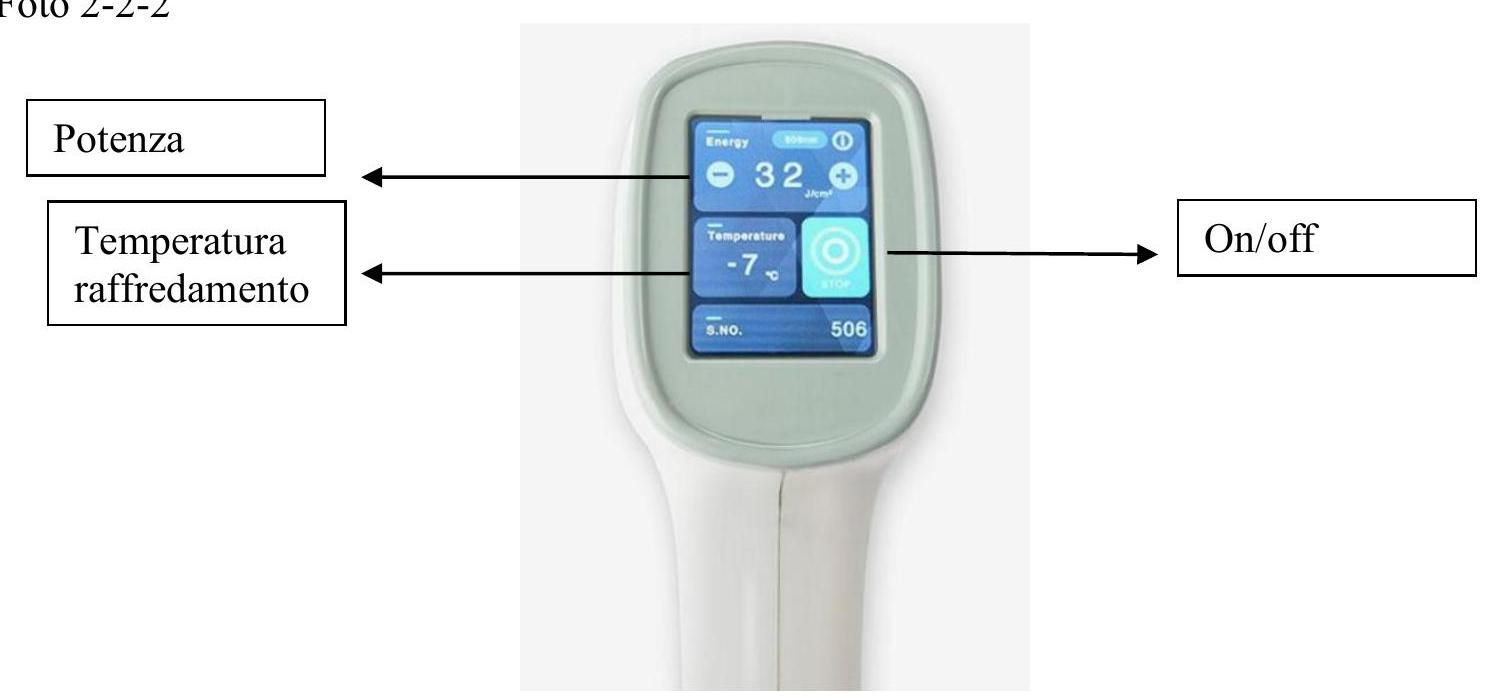
\includegraphics[alt={},max width=\textwidth]{0673f156-6613-4c24-ad16-c1dd5450a875-07_700_1486_1532_424}
\end{center}
\end{figure}

Display LCD della maniglia: densità di potenza, temperatura di raffreddamento della maniglia, informazioni sulla maniglia, lavoro di avvio o spegnimento, numero di tiro. Il display a cristalli liquidi può regolare la potenza del laser e controllare il laser avviandolo/spegnendolo.

Specifiche per Android-SmartDepi\\
Specifiche per Android-SmartDepi

\begin{table}[h]
\begin{center}
\captionsetup{labelformat=empty}
\caption{Tabella 2-2-1 Specifiche dell'attrezzatura}
\begin{tabular}{|l|l|}
\hline
Modello/Lunghezza d'onda & Laser 808 / 755/808/940/1064nm \\
\hline
potenza laser & $1200 \mathrm{~W} / 1600 \mathrm{~W}$ (personalizzabile) \\
\hline
dimensione in punti & $15 \mathrm{~mm}^{*} 20 \mathrm{~mm} /$ \\
\hline
Gestisci le dimensioni dello schermo & \begin{tabular}{l}
Touch screen LCD da 2,1 pollici + \\
schermo da 1,3 pollici \\
\end{tabular} \\
\hline
Dimensioni dello schermo della macchina & \begin{tabular}{l}
Schermo Android da 13,3 pollici \\
(esclusivo) \\
\end{tabular} \\
\hline
densita 'energia & $10-40 \mathrm{~J} /$ CM2 \\
\hline
\end{tabular}
\end{center}
\end{table}

\begin{center}
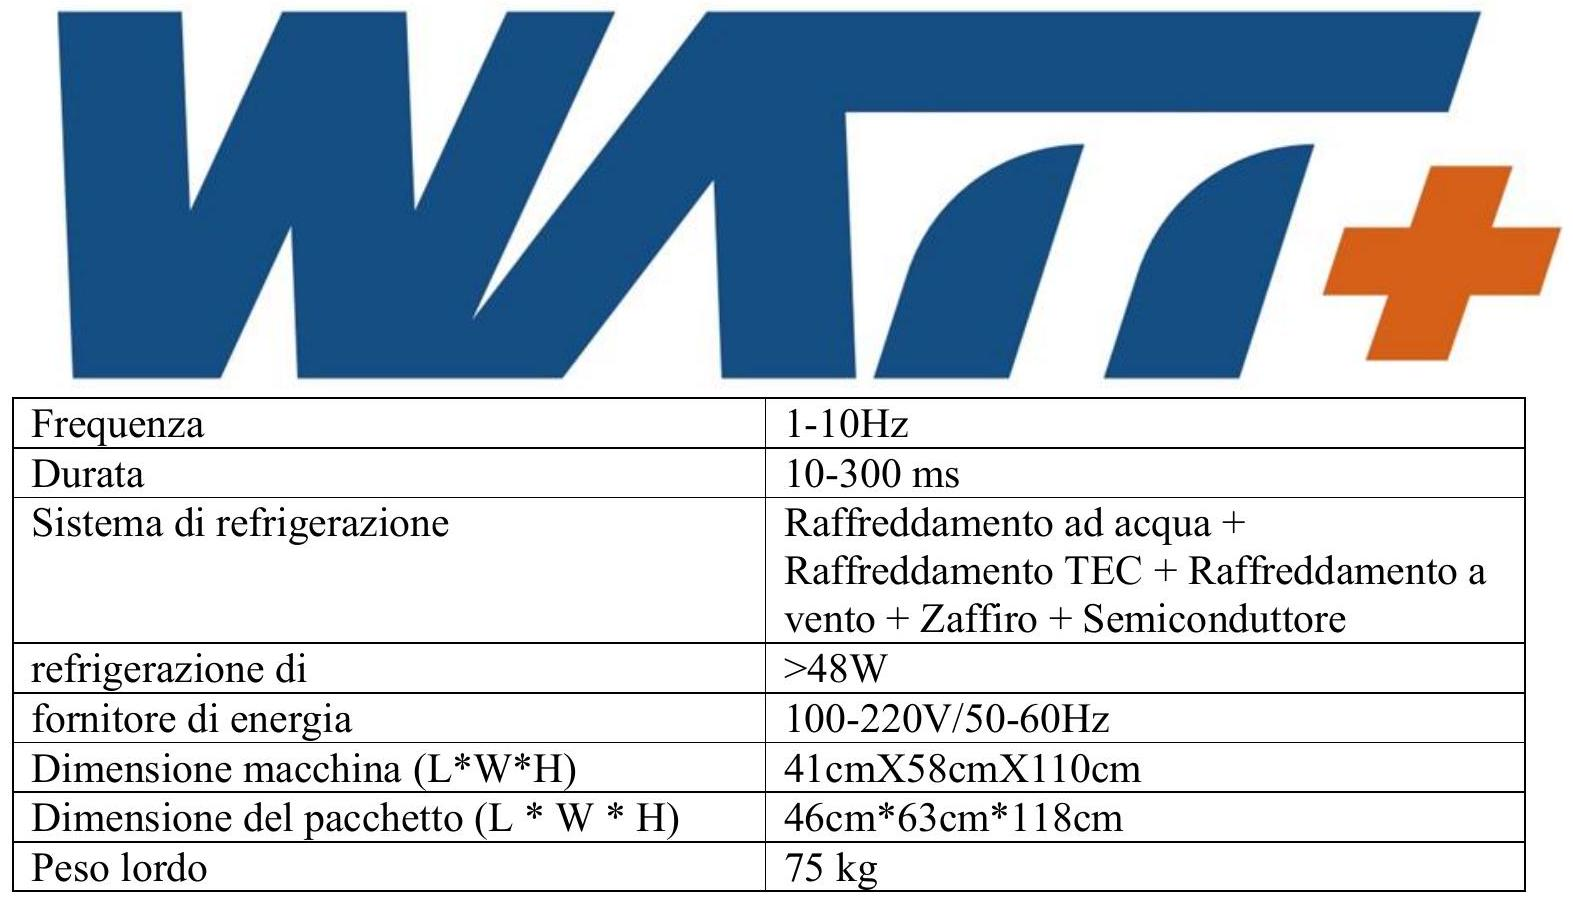
\includegraphics[max width=\textwidth, alt={}]{0673f156-6613-4c24-ad16-c1dd5450a875-09_901_1573_11_264}
\end{center}

Capitolo 3 Installazione di un impianto\\
3.1 Processo di installazione delle apparecchiature

L'apparecchiatura deve essere installata in un ambiente privo di gas corrosivi, polvere e meno particelle, che possono causare danni ai componenti elettronici e ottici e ai cavi dell'apparecchiatura. Più polvere e particelle nell'aria possono anche causare danni ai filtri e ai componenti elettrici.

L'intervallo di temperatura e umidità dell'ambiente di installazione dell'apparecchiatura deve soddisfare i requisiti dei parametri di prestazione dell'apparecchiatura.

\begin{itemize}
  \item Aprire la confezione del dispositivo,
  \item Conservare le attrezzature al chiuso per un giorno, evitando l'umidità eccessiva e i danni causati dal trasporto su lunghe distanze.
  \item Quando l'umidità dell'apparecchio è adeguata, assemblare i componenti dell'apparecchio per garantire una connessione stabile.
  \item Riempire il serbatoio con acqua distillata.
  \item Collegare la maniglia di elaborazione del dispositivo alla fonte di alimentazione del dispositivo.
  \item Dopo che tutti i componenti e l'alimentazione sono stati collegati, accendere il dispositivo e verificarne le prestazioni, assicurandosi che il dispositivo sia collegato correttamente e con parametri.
\end{itemize}

\subsection{Requisiti di installazione e quantità di acqua immessa}
Quando si installano i componenti dell'apparecchiatura, la prima operazione è quella di iniettare acqua nell'apparecchiatura. L'apparecchiatura deve essere eseguita prima di ogni operazione

Controllare se il segno dell'acqua nel sito di iniezione dell'acqua dell'apparecchiatura è maggiore del $90 \%$ della colonna d'acqua. Se non viene raggiunto, deve essere riempito con acqua distillata.

\subsubsection{Direttiva sulle acque di scarico}
Quando l'apparecchiatura funziona, la temperatura ambiente esterna deve essere compresa tra $5^{\circ} \mathrm{C}$ e $40^{\circ} \mathrm{C}$, l'umidità non deve essere superiore all' $80 \%$ e la sala di trattamento deve essere mantenuta pulita in ogni momento.

Assicurarsi che le prese d'aria siano aperte prima di iniettare acqua e che l'utensile manuale sia assemblato (vedere 3.2.3 Installazione della maniglia di maniglia), altrimenti non è possibile iniettare acqua, come mostrato nella figura.\\
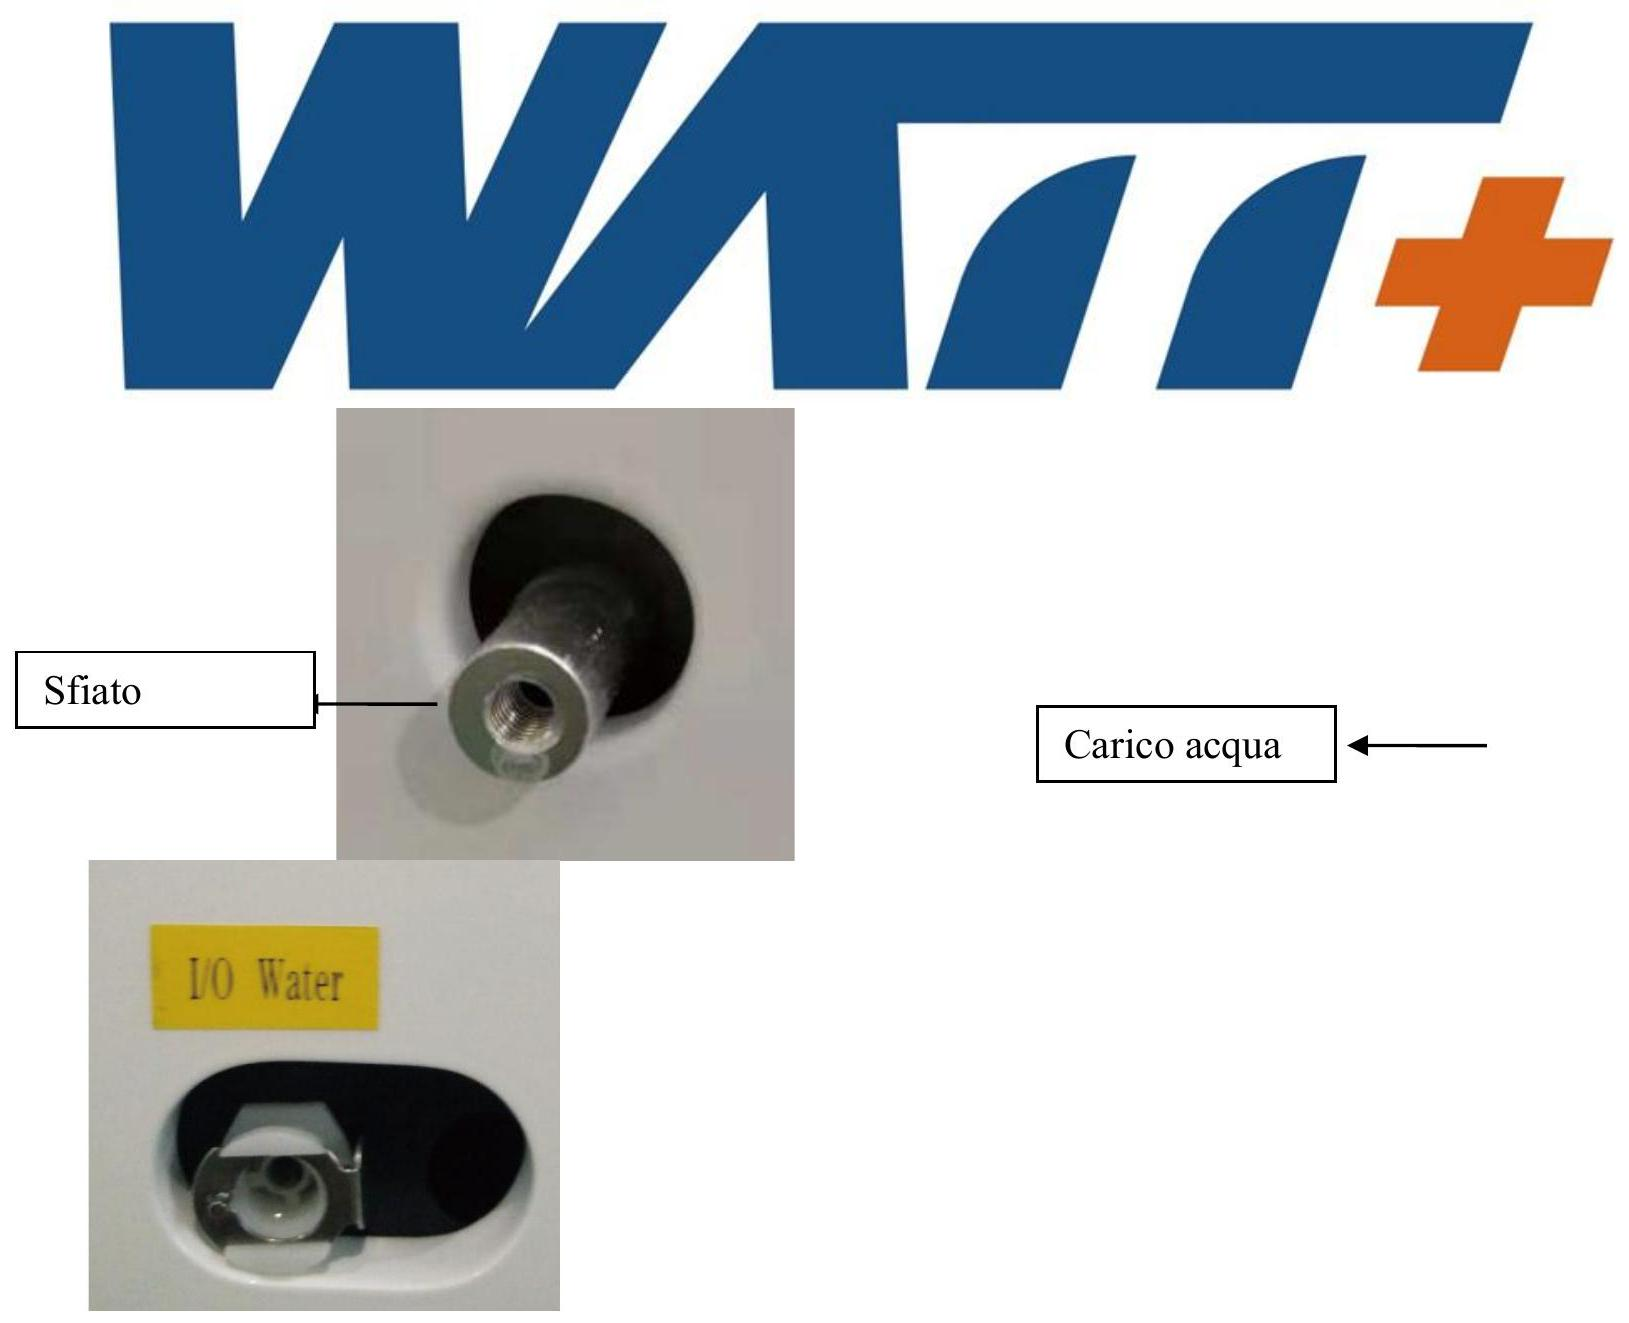
\includegraphics[max width=\textwidth, alt={}, center]{0673f156-6613-4c24-ad16-c1dd5450a875-11_1323_1629_0_212}\\
VILA

Inserire la porta del giunto bianco dell'imbuto nel foro di iniezione dell'acqua e, quando entra il tubo di iniezione dell'acqua, iniettare acqua nel dispositivo attraverso l'imbuto.

Quando la posizione raggiunge H o c'è una fuoriuscita d'acqua, l'iniezione dell'acqua termina come mostrato nella figura.\\
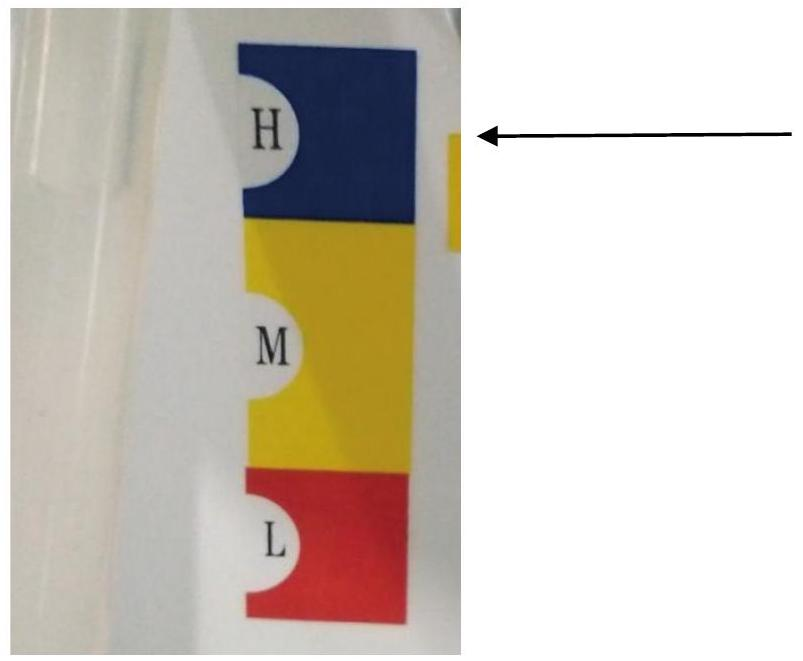
\includegraphics[max width=\textwidth, alt={}, center]{0673f156-6613-4c24-ad16-c1dd5450a875-12_661_803_687_413}

Una volta completata l'iniezione dell'acqua, premere la piastra di ferro sul foro di drenaggio per rimuovere il dispositivo di iniezione dell'acqua.

\subsubsection{Prove del ciclo dell'acqua}
Dopo che l'apparecchiatura è stata riempita con acqua, collegare la linea di alimentazione e la linea del piede e, dopo aver collegato, eseguire il debug del ciclo dell'acqua dell'apparecchiatura.

I passaggi per la messa in servizio del ciclo dell'acqua sono i seguenti:\\
Prima dell'avvio del dispositivo, l'interruttore di arresto di emergenza deve essere in uno stato non \href{http://premuto.Se}{premuto.Se} l'interruttore di arresto di emergenza è in uno stato premuto, fare clic sul pulsante di arresto di emergenza per mantenerlo in uno stato non premuto.

Impostare l'interruttore dell'interruttore sul retro dell'unità in posizione "ON".\\
Ruotare l'interruttore a pulsante in senso orario e il sistema di raffreddamento della circolazione dell'acqua interna dell'apparecchiatura funziona automaticamente.\\
VICRO

Osservare se il ciclo dell'acqua dell'apparecchiatura funziona normalmente.\\
Se non ci sono perdite d'acqua, allarmi idrici, ecc., Lascia che il dispositivo funzioni automaticamente per più di un minuto e puoi usarlo.

Nota: cambiare l'acqua ogni 2-3 mesi. Il filtro deve essere sostituito quando si cambia l'acqua. Rimuovere quanta più acqua possibile dal sistema di raffreddamento.

\subsubsection{Installazione delle maniglie di movimentazione}
Quando si installa la maniglia di elaborazione, posizionare la maniglia sotto il corpo principale in modo che le bolle d'aria vengano scaricate dalla maniglia.Dopo l'installazione, avviare il dispositivo e far circolare l'acqua per almeno un minuto prima dell'elaborazione.

Allineare la maniglia con l'interfaccia come mostrato, quindi ruotare il pulsante a destra fino a quando non è serrato e non può più essere ruotato a destra.\\
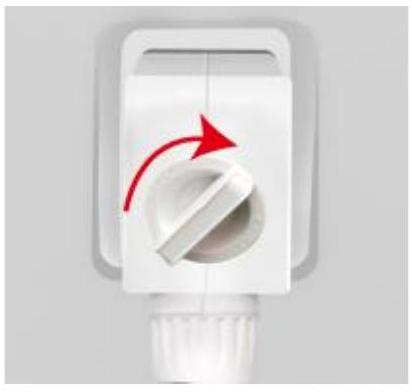
\includegraphics[max width=\textwidth, alt={}, center]{0673f156-6613-4c24-ad16-c1dd5450a875-14_392_412_1073_950}

Quando la maniglia deve essere rimossa, girare a sinistra fino a quando la maniglia non è allentata ed estratta. Quindi la maniglia di elaborazione può essere rimossa.\\
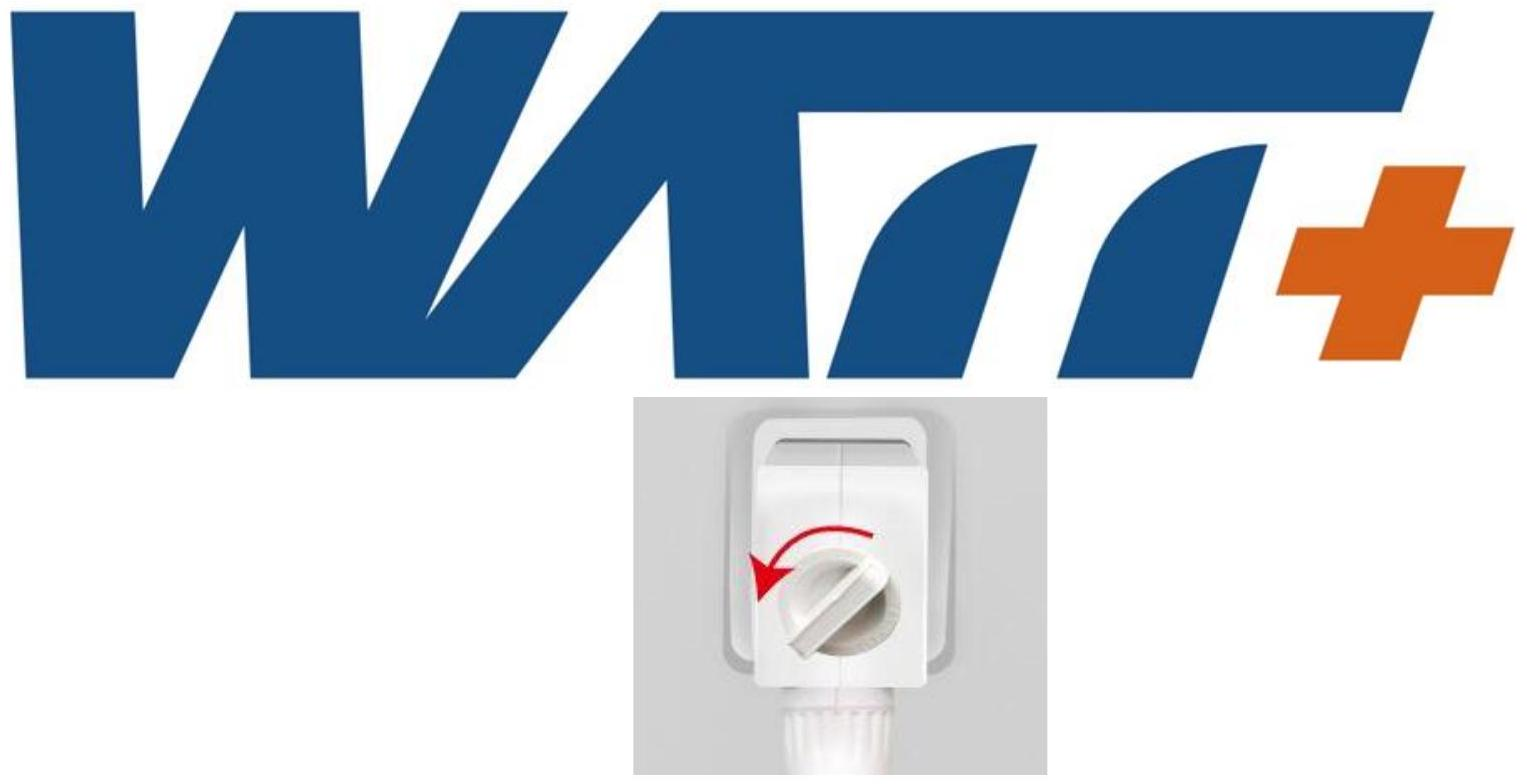
\includegraphics[max width=\textwidth, alt={}, center]{0673f156-6613-4c24-ad16-c1dd5450a875-15_784_1527_11_311}

Capitolo 4 Istruzioni per l'uso del software\\
4.1 Interfaccia di lavoro\\
4.1.1 Istruzioni per il display di lavoro

\begin{center}
\begin{tabular}{|l|l|l|}
\hline
» Immagini & Nome e cognome & La funzione \\
\hline
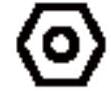
\includegraphics[max width=\textwidth, alt={}]{0673f156-6613-4c24-ad16-c1dd5450a875-16_91_111_545_494}
 & Impostazioni del sistema & Immettere le impostazioni di sfondo \\
\hline
L & Temperatura dell'acqua & Visualizzazione in tempo reale della temperatura del serbatoio dell'acqua \\
\hline
7 & Temperatura della maniglia & Visualizzazione della temperatura della maniglia in tempo reale \\
\hline
\# & La corrente d'acqua & Visualizzazione del flusso d'acqua in tempo reale \\
\hline
\end{tabular}
\end{center}

W $/ \sqrt{6}+$

\begin{center}
\begin{tabular}{|l|l|l|}
\hline
ヒ & Livello dell'acqua & Visualizza il livello dell'acqua in tempo reale \\
\hline
$\mathbf{J} / \mathbf{c m}^{\mathbf{2}}$ & Densità di energia & Visualizzazione della densità di energia in tempo reale \\
\hline
MS & Durata dei lavori & Mostra la durata in tempo reale \\
\hline
HZ & La frequenza & Frequenza di visualizzazione in tempo reale \\
\hline
7) & Immagine vocale & Suggerimenti vocali \\
\hline
(•) & Preparazione del lavoro & Pronto per iniziare i lavori \\
\hline
Tenor & Preparazione della macchina & Preparazione della macchina \\
\hline
146 & Immagine della depilazione & Visualizzazione durante la funzione di depilazione \\
\hline
a & Immagine di ringiovanimento della pelle & Visualizzazione durante la funzione di ringiovanimento della pelle \\
\hline
D & Memorizza le immagini dei dati & Archiviazione dei dati \\
\hline
祭 & Selezione del livello di raffreddamento & Regolazione dell'effetto di raffreddamento a 5 velocità \\
\hline
(8) & Login utente & Login utente \\
\hline
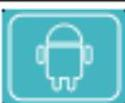
\includegraphics[max width=\textwidth, alt={}]{0673f156-6613-4c24-ad16-c1dd5450a875-17_103_125_2242_501}
 & Torna al desktop & Toma al desktop \\
\hline
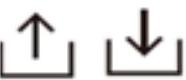
\includegraphics[max width=\textwidth, alt={}]{0673f156-6613-4c24-ad16-c1dd5450a875-17_80_186_2410_469}
 & Caricamento e download dei dati & Possibilità di caricare e scaricare dati tramite interfaccia USB \\
\hline
\end{tabular}
\end{center}

\begin{center}
\begin{tabular}{|l|l|l|}
\hline

\includegraphics[max width=\textwidth, alt={}]{0673f156-6613-4c24-ad16-c1dd5450a875-18_148_155_584_432}
 & Avviso di temperatura dell'acqua & Quando il valore mostrato nel diagramma della temperatura del serbatoio è troppo alto, l'immagine diventa rossa \\
\hline

\includegraphics[max width=\textwidth, alt={}]{0673f156-6613-4c24-ad16-c1dd5450a875-18_150_155_805_432}
 & Gestione degli avvisi di temperatura & L'immagine diventa rossa quando il valore mostrato nel diagramma della temperatura della fessura della maniglia è troppo alto \\
\hline
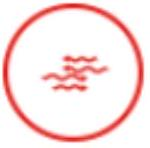
\includegraphics[max width=\textwidth, alt={}]{0673f156-6613-4c24-ad16-c1dd5450a875-18_148_150_1033_437}
 & Allarme di flusso d'acqua & Quando il valore mostrato nel diagramma della temperatura del serbatoio è troppo alto, l'immagine diventa rossa \\
\hline

\includegraphics[max width=\textwidth, alt={}]{0673f156-6613-4c24-ad16-c1dd5450a875-18_151_114_1256_441}
 & Avviso serbatoio acqua & L'icona diventa rossa quando il valore visualizzato nell'immagine dell'indicatore del serbatoio è troppo alto \\
\hline
\end{tabular}
\end{center}

4.1.2 Descrizione dell'interfaccia di lavoro\\
4.1.2.1 Allerta sul livello dell'acqua

Quando l'immagine nell'avviso di livello dell'acqua viene visualizzata in rosso, indica un allarme di livello dell'acqua e il livello dell'acqua del serbatoio dell'acqua è troppo basso. Trattamento: aggiungere acqua in tempo.

\section{$\sqrt{1} \times 2+$}
\subsubsection{Avvertenze sul serbatoio dell'acqua}
Quando il valore di visualizzazione dell'immagine dell'indicatore di temperatura del serbatoio dell'acqua è troppo alto, l'immagine viene visualizzata in rosso, indicando l'allarme di temperatura del serbatoio dell'acqua e il sistema spegne automaticamente l'interruttore per entrare nello stato di standby. Metodo di trattamento: verificare che i componenti del sistema di circolazione dell'acqua funzionino correttamente e siano danneggiati. Se non si verifica la situazione di cui sopra, si prega di contattare il rivenditore.\\
4.1.2.3 Gestione delle avvertenze di temperatura

Quando l'icona dell'indicatore del flusso d'acqua mostra un valore inferiore a " 1 " e la goccia d'acqua nell'icona è illuminata, indica un allarme di flusso d'acqua e il sistema passa automaticamente allo stato di standby.

Metodo di trattamento: osservare i segni dell'acqua, vedere se l'acqua è sufficiente o verificare se la connessione tra la maniglia di trattamento e il dispositivo perde acqua. Se non si verifica nulla di quanto sopra, si prega di contattare il personale di manutenzione post-vendita.

\subsubsection{Avviso di flusso d'acqua}
Quando il valore visualizzato nell'icona dell'indicatore di temperatura della testa di elaborazione è troppo alto e "!" Appare nell'icona che indica l'allarme di temperatura della testa di elaborazione e il sistema passa automaticamente allo stato di standby.

Soluzione: riavviare l'unità dopo che la maniglia di elaborazione è stata interrotta per un po '. Se l'allarme di temperatura della testa di elaborazione persiste, contattare il personale di assistenza post-vendita.\\
4.2 Visualizzazione e descrizione dell'interfaccia front-end.\\
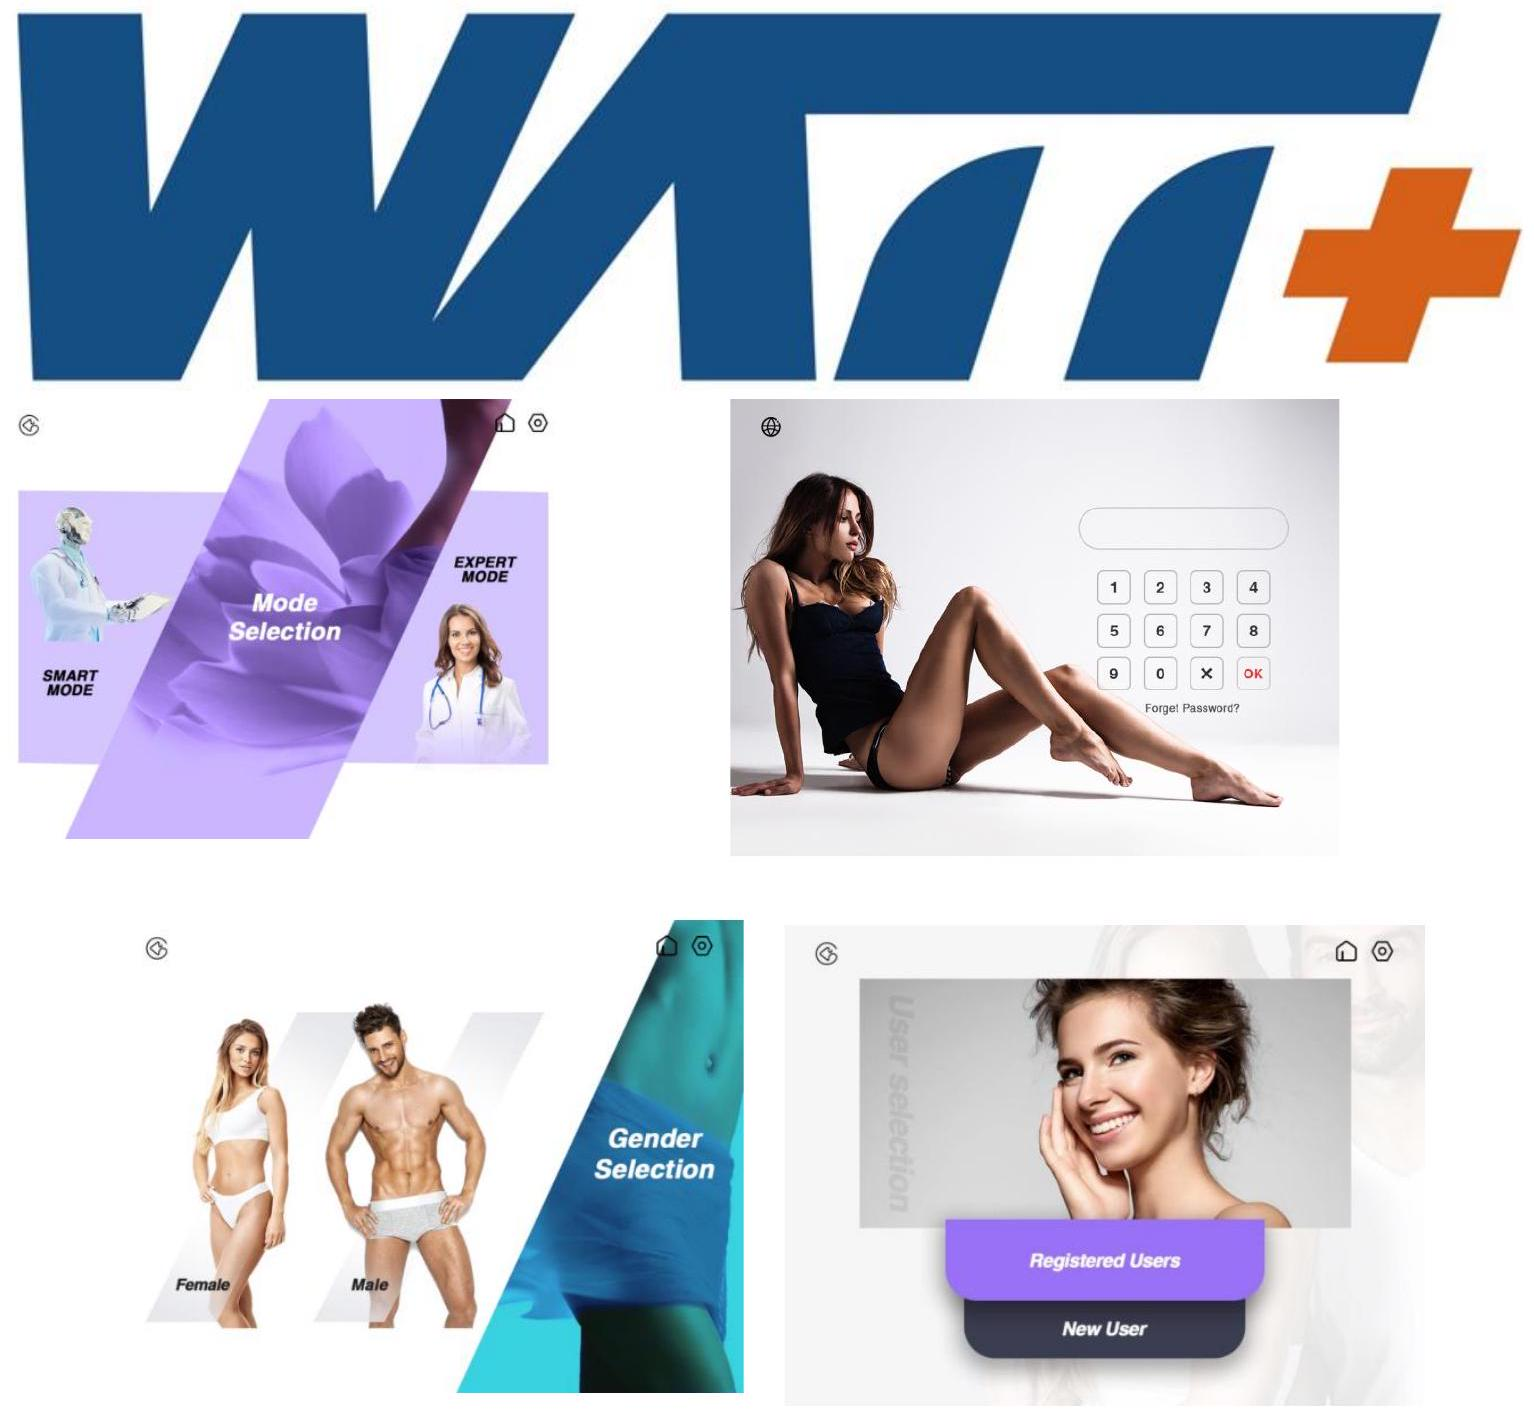
\includegraphics[max width=\textwidth, alt={}, center]{0673f156-6613-4c24-ad16-c1dd5450a875-20_1419_1534_9_304}\\
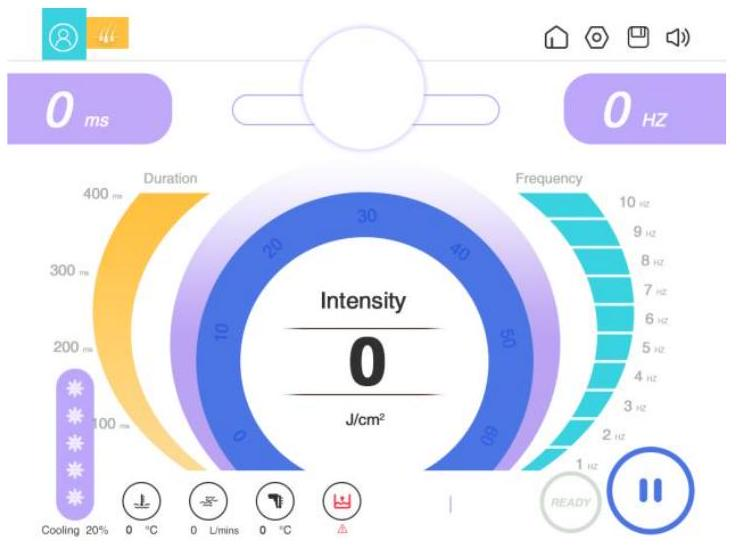
\includegraphics[max width=\textwidth, alt={}, center]{0673f156-6613-4c24-ad16-c1dd5450a875-20_554_739_1523_292}\\
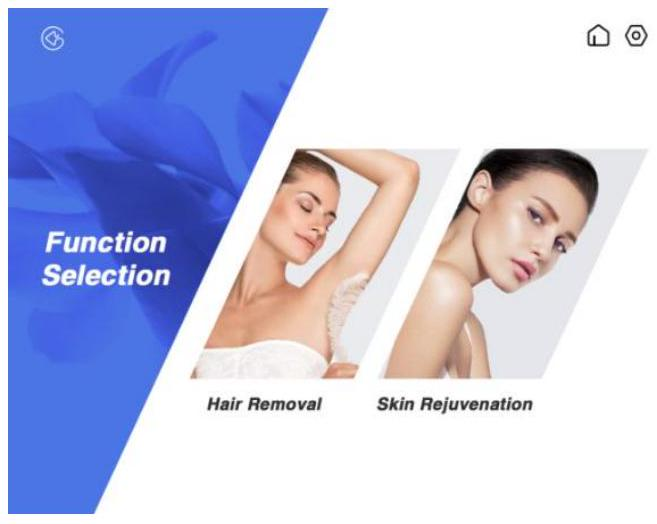
\includegraphics[max width=\textwidth, alt={}, center]{0673f156-6613-4c24-ad16-c1dd5450a875-20_524_657_1562_1048}\\
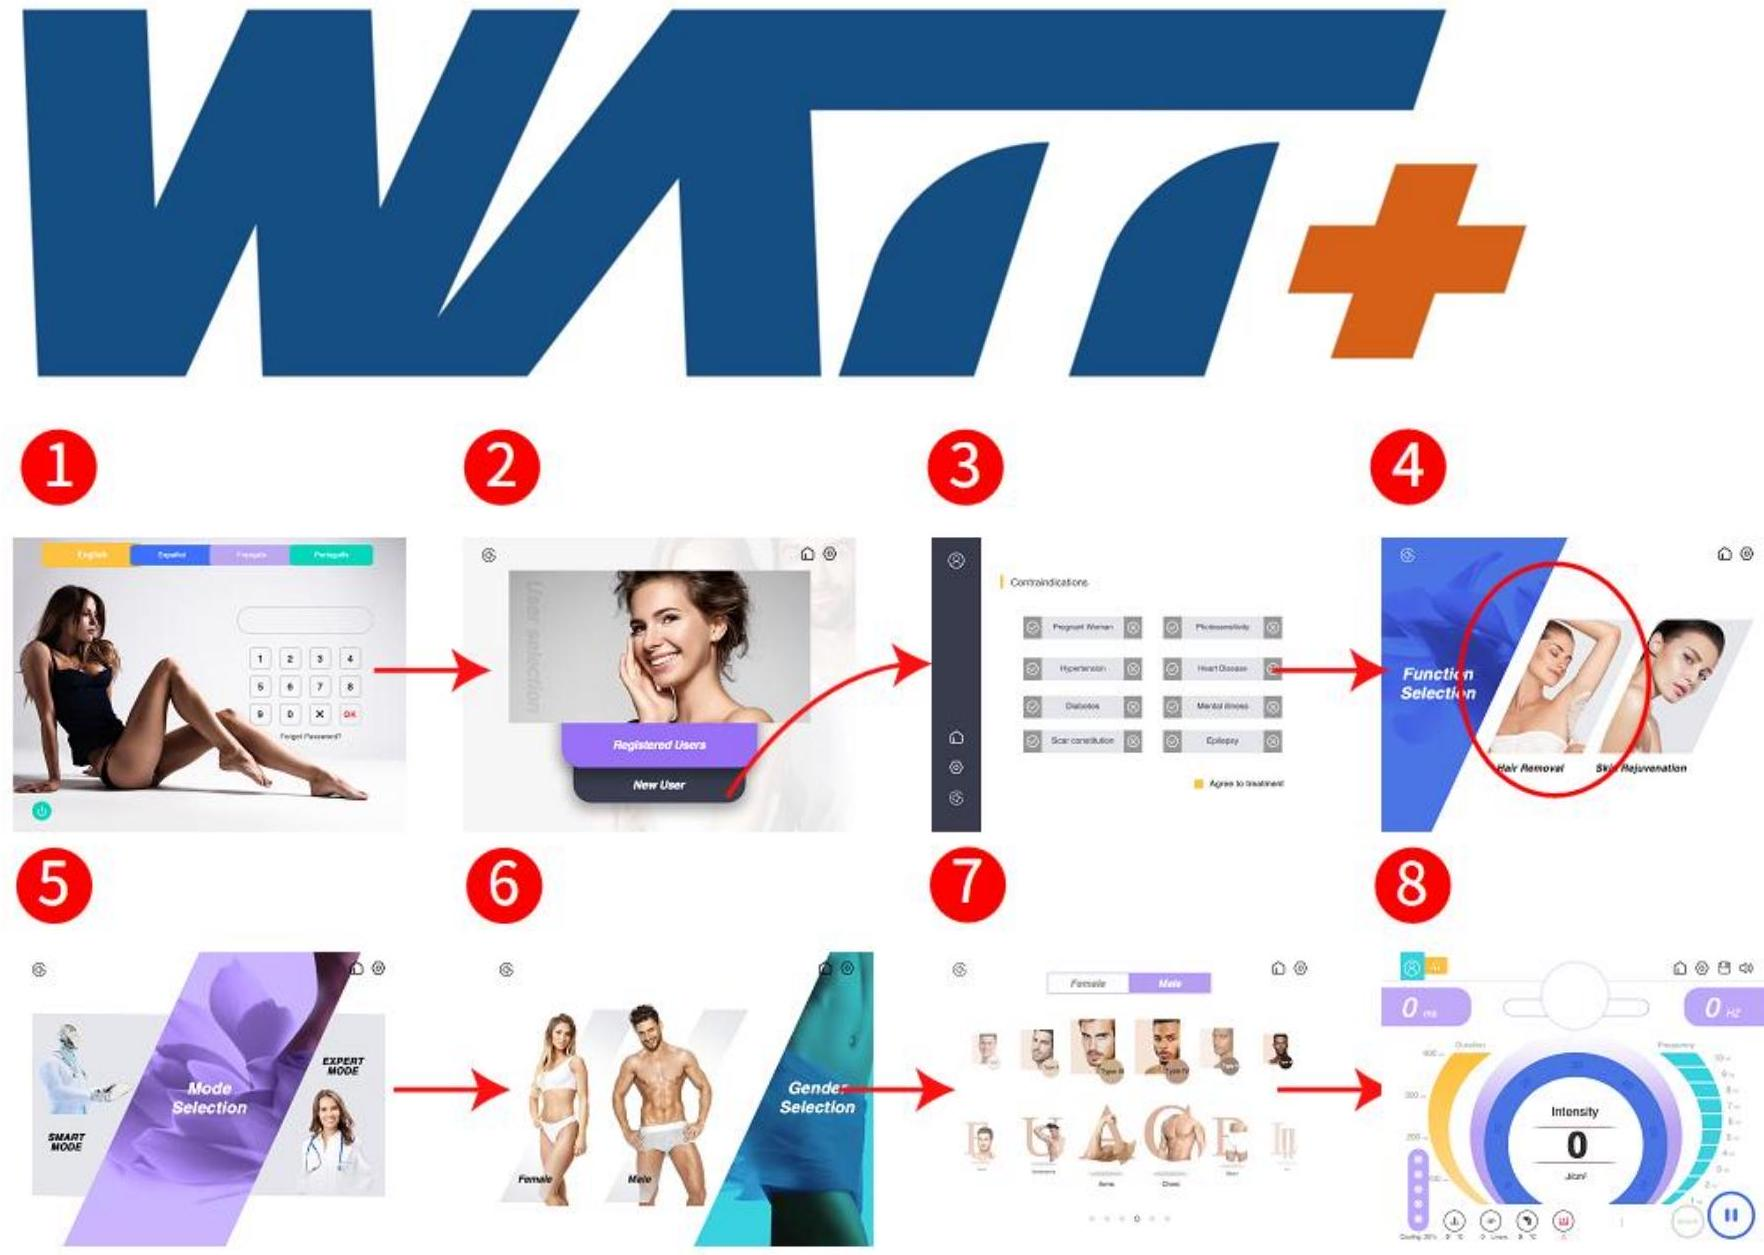
\includegraphics[max width=\textwidth, alt={}, center]{0673f156-6613-4c24-ad16-c1dd5450a875-21_1255_1764_13_299}

Come mostrato nella figura, Per prima cosa accedi all'interfaccia della password per accedere alla selezione dell'utente vecchio e nuovo. Seleziona un nuovo utente per accedere all'interfaccia di selezione delle controindicazioni per accedere all'interfaccia di selezione delle funzioni, selezionare la selezione della modalità di accesso alla depilazione, selezionare la modalità intelligente per accedere all'interfaccia di selezione del genere, inserire la parte di accesso e l'interfaccia di selezione del colore della pelle per accedere all'interfaccia operativa principale, il sistema genera automaticamente i parametri richiesti, fare clic su Lavora\\
4.2.2 Descrizione dell'interfaccia di depilazione (nuovo utente + depilazione + processo interattivo dell'interfaccia utente in modalità esperta)\\
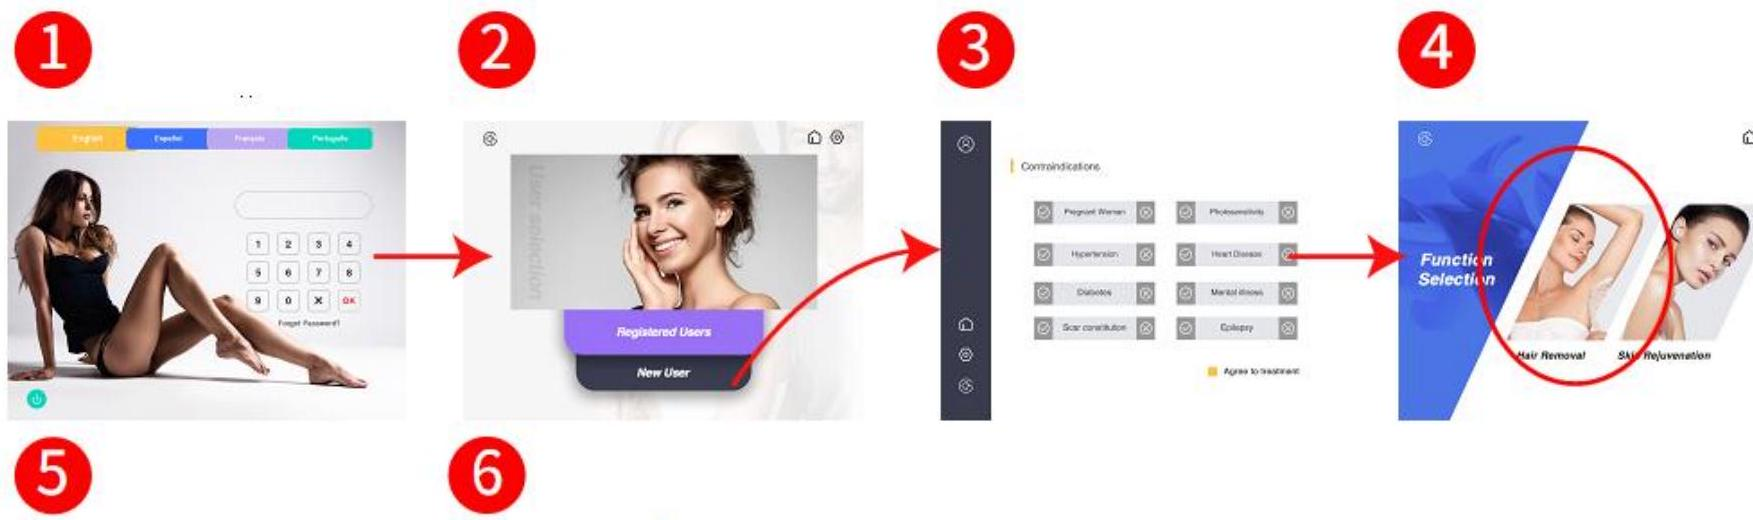
\includegraphics[max width=\textwidth, alt={}, center]{0673f156-6613-4c24-ad16-c1dd5450a875-22_520_1753_703_310}\\
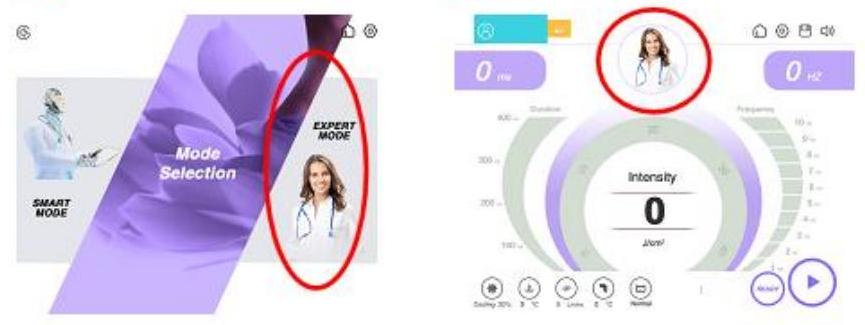
\includegraphics[max width=\textwidth, alt={}, center]{0673f156-6613-4c24-ad16-c1dd5450a875-22_325_865_1231_319}

Come mostrato in figura, prima di tutto accedere all'interfaccia password per accedere alla selezione utente vecchio e nuovo, selezionare il nuovo utente per accedere all'interfaccia di selezione controindicazioni per accedere all'interfaccia di selezione funzione, selezionare la selezione della modalità di accesso depilazione, selezionare la modalità esperto per accedere all'interfaccia operativa principale esperto, nessun valore,

l'operatore regola i parametri richiesti in base alla propria esperienza, fare clic sul posto di lavoro, pronto per l'uso.\\
4.2.3 Descrizione dell'interfaccia per il ringiovanimento della pelle (nuovo utente + processo interattivo dell'interfaccia utente per il ringiovanimento della pelle)\\
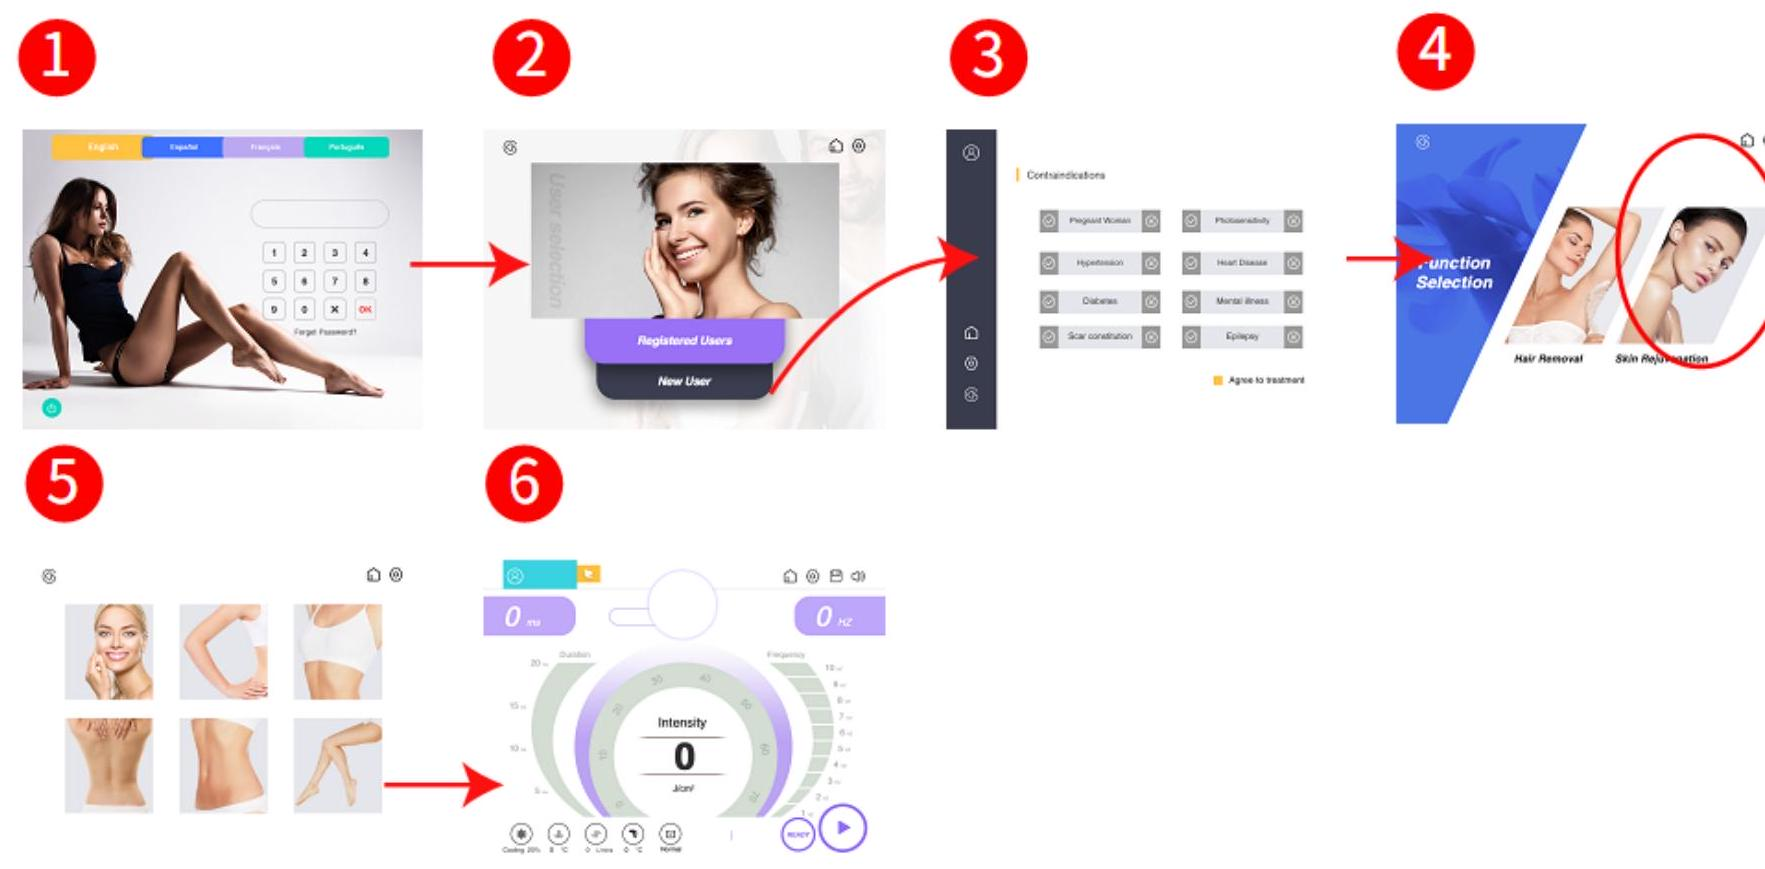
\includegraphics[max width=\textwidth, alt={}, center]{0673f156-6613-4c24-ad16-c1dd5450a875-23_869_1765_753_301}

Come mostrato nella figura, prima accedi all'interfaccia della password per accedere alla selezione dell'utente vecchio e nuovo, seleziona il nuovo utente per\\
Whate\\
accedere all'interfaccia di selezione della controindicazione per accedere all'interfaccia di selezione della funzione, seleziona la selezione della parte di ingresso del ringiovanimento della pelle, entra nell'interfaccia operativa principale, il sistema genera automaticamente i parametri richiesti, fai clic sul lavoro per usarlo\\
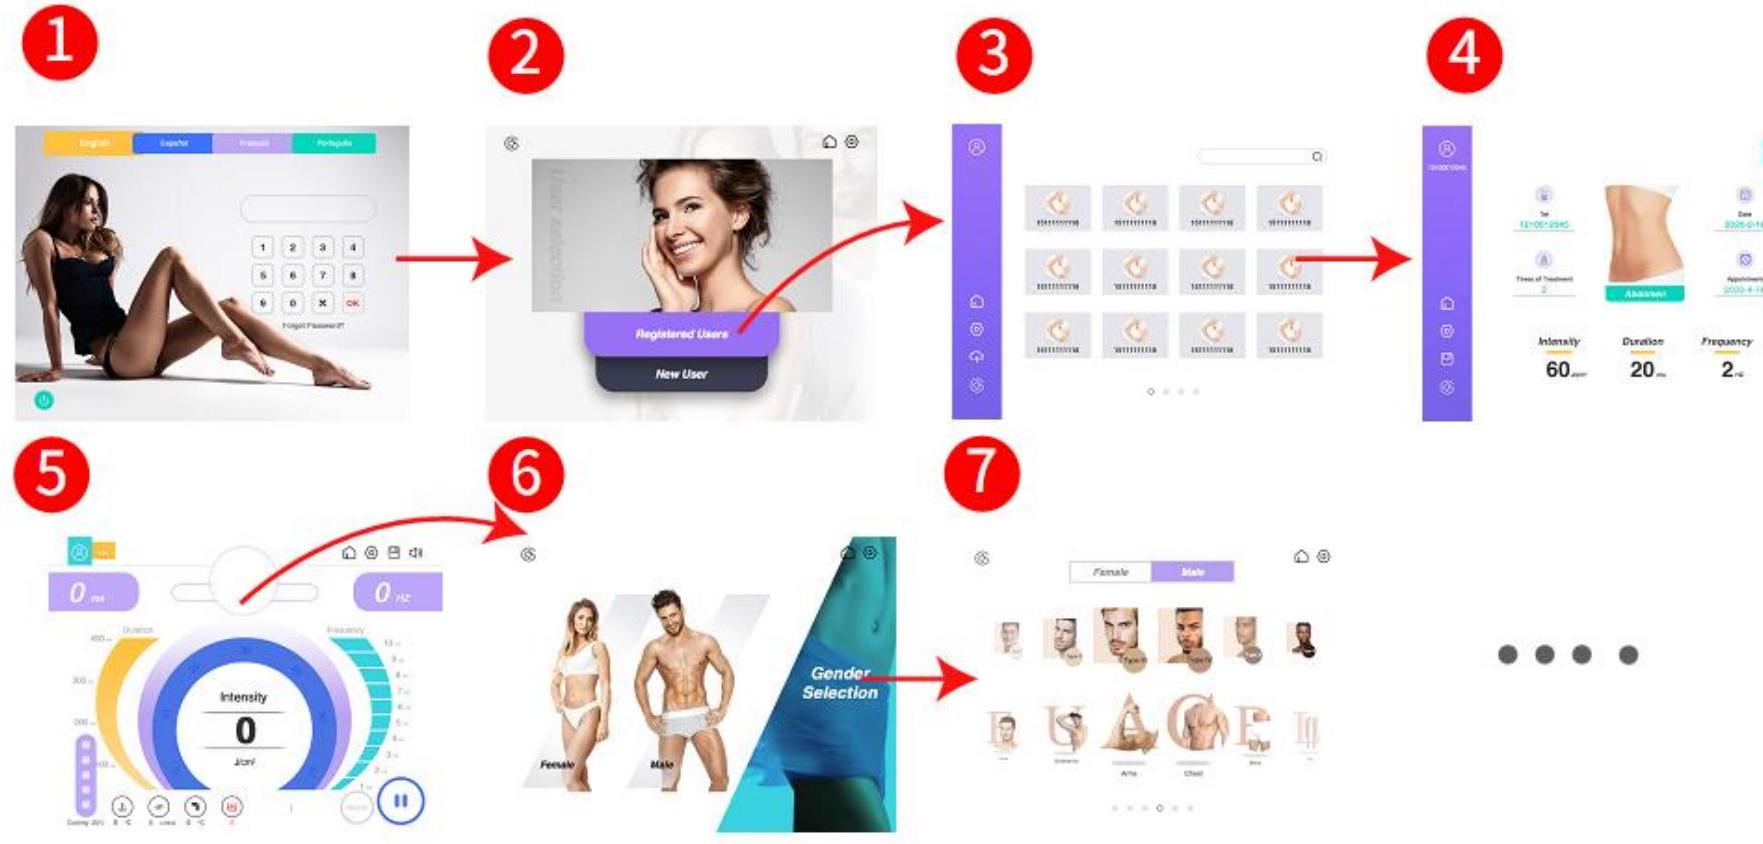
\includegraphics[max width=\textwidth, alt={}, center]{0673f156-6613-4c24-ad16-c1dd5450a875-24_844_1763_712_303}

Come mostrato nella figura, accedi prima all'interfaccia della password per accedere alla selezione dell'utente vecchio e nuovo, seleziona il vecchio utente per accedere all'interfaccia di selezione dell'elenco clienti per accedere all'interfaccia della pagina dei\\
dettagli del cliente per accedere alla selezione del genere per inserire la selezione della posizione...\\
4.2.5 Descrizione dell'interfaccia (salvare le informazioni sui nuovi utenti)\\
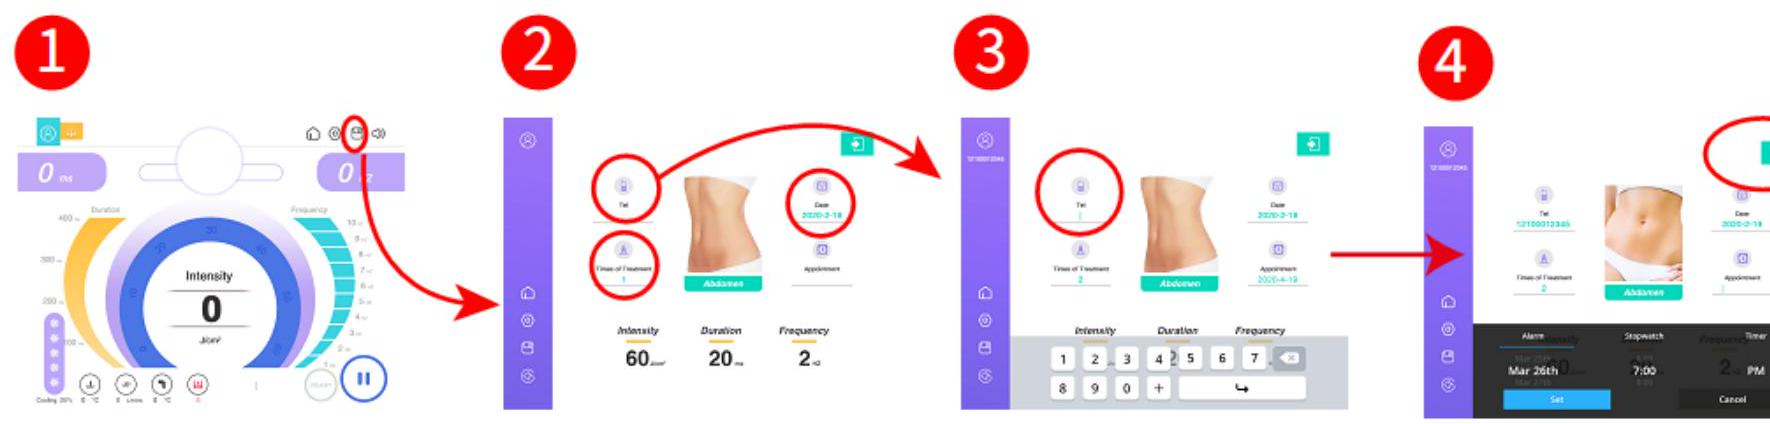
\includegraphics[max width=\textwidth, alt={}, center]{0673f156-6613-4c24-ad16-c1dd5450a875-25_424_1770_614_296}\\
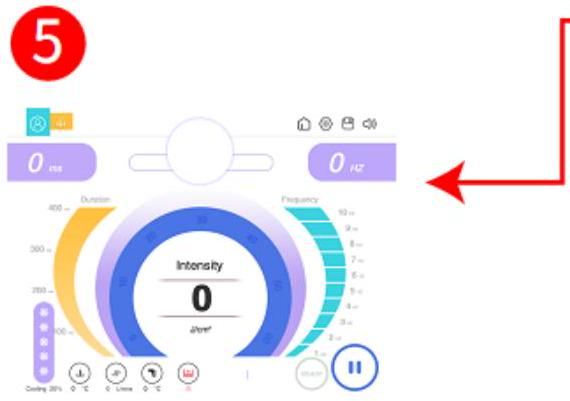
\includegraphics[max width=\textwidth, alt={}, center]{0673f156-6613-4c24-ad16-c1dd5450a875-25_401_570_1046_303}\\
4.2.6 Descrizione dell'interfaccia (salvataggio delle informazioni del vecchio utente)\\
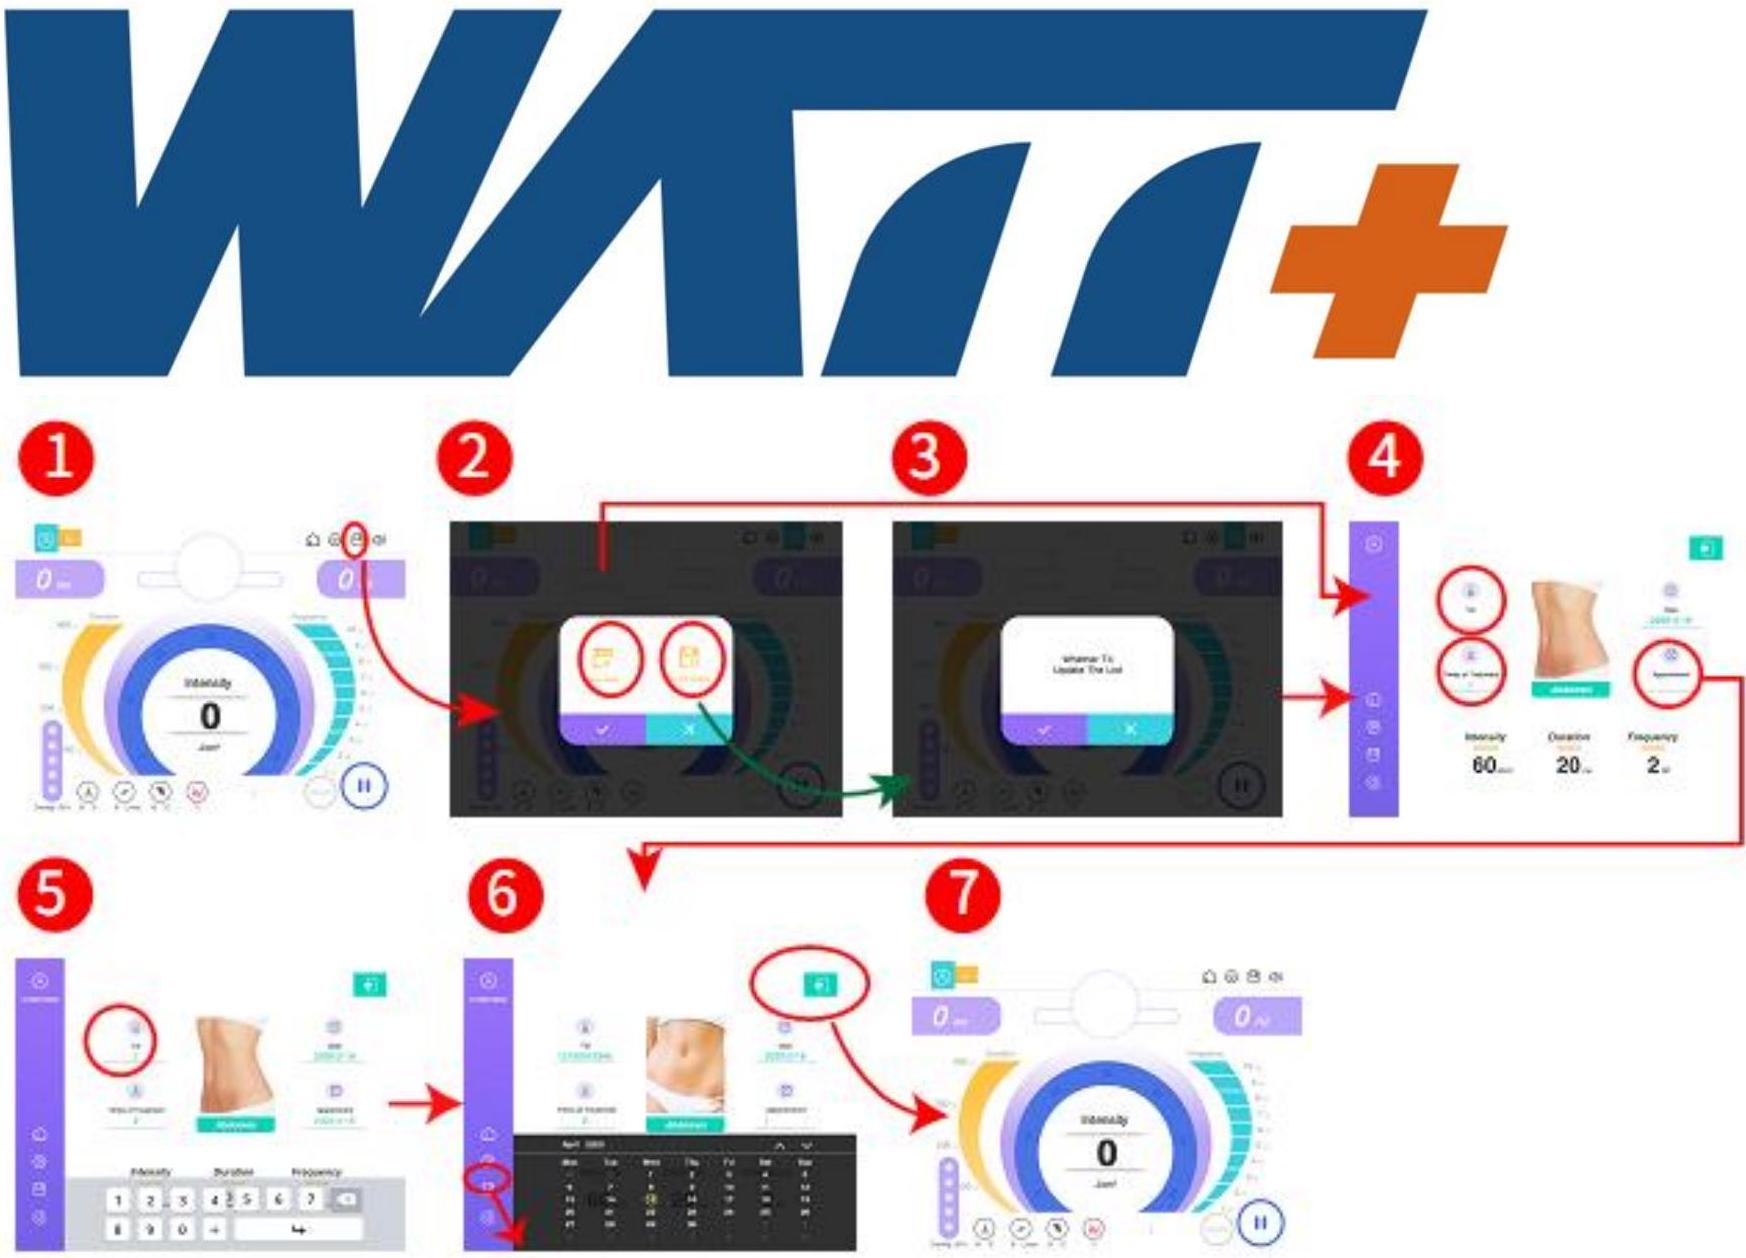
\includegraphics[max width=\textwidth, alt={}, center]{0673f156-6613-4c24-ad16-c1dd5450a875-26_1258_1746_13_317}

Come mostrato nella figura, selezionare innanzitutto il pulsante Salva nell'interfaccia operativa principale per selezionare Salva Aggiungi o Salva aggiornamento Seleziona Salva aggiornamento Pulsante di conferma aggiornamento Pagina dei dettagli dell'utente Aggiungi telefono Aggiungi la data di trattamento successiva e torna all'interfaccia operativa principale per il trattamento.

\subsubsection{Visualizzazione e descrizione dell'interfaccia in background}
\begin{figure}[h]
\begin{center}
  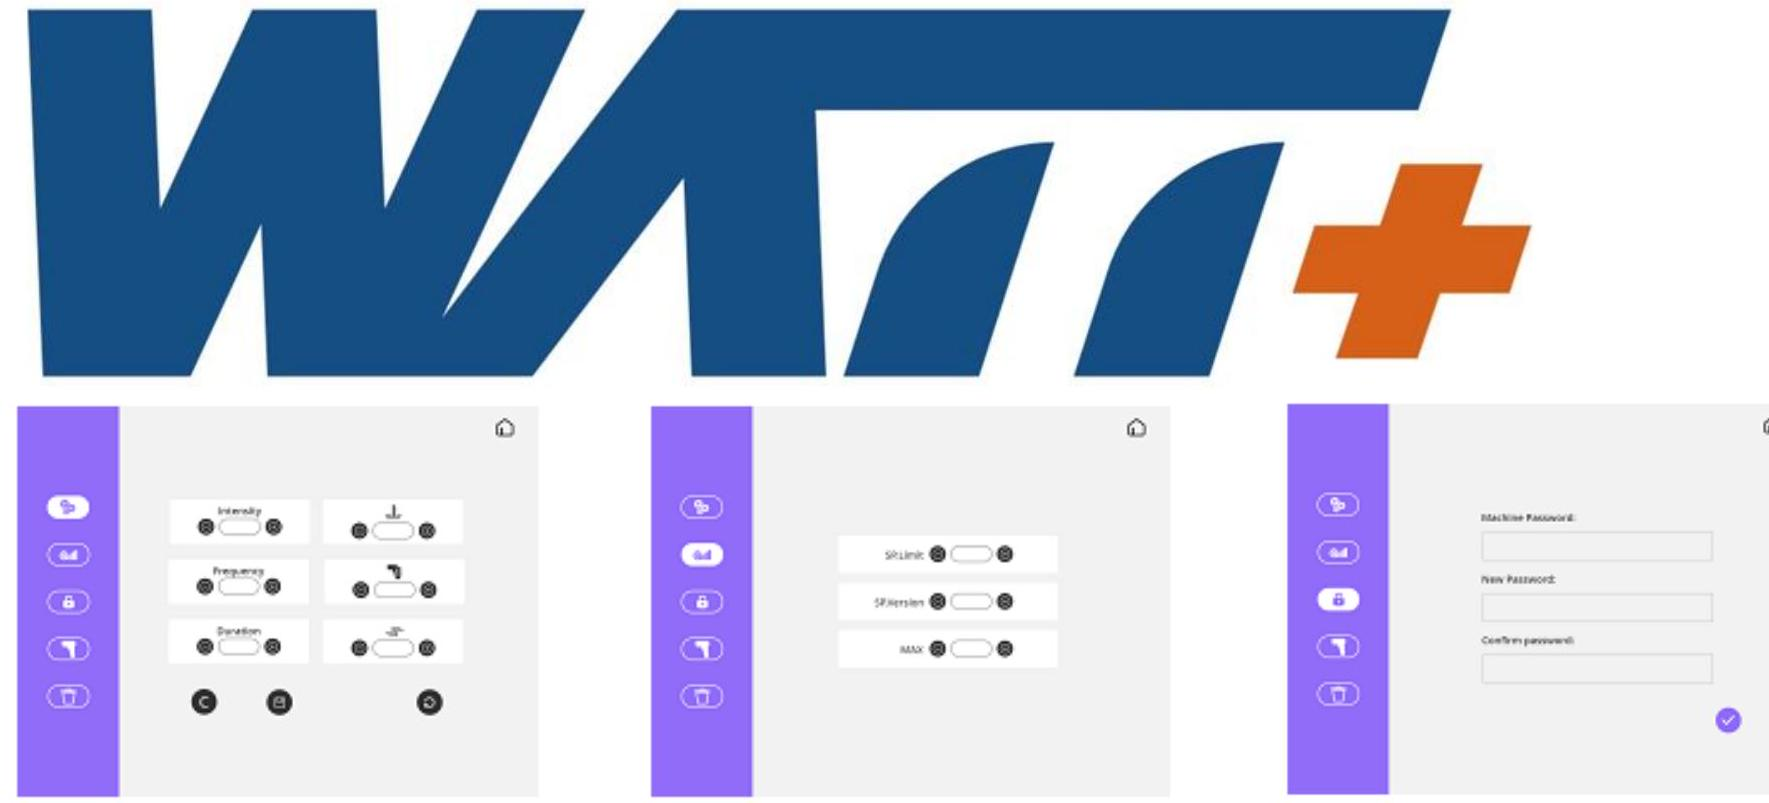
\includegraphics[alt={},max width=\textwidth]{0673f156-6613-4c24-ad16-c1dd5450a875-27_803_1769_13_294}
\captionsetup{labelformat=empty}
\caption{Funzione di impostazione dei parametri Funzione di impostazione dell'energia e dei limiti Funzione di impostazione del cambio di password}
\end{center}
\end{figure}

\begin{figure}[h]
\begin{center}
  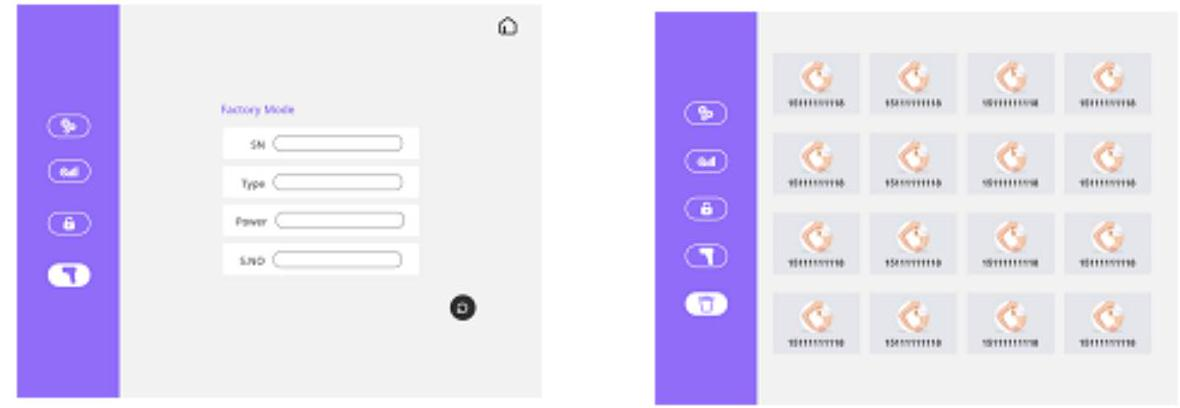
\includegraphics[alt={},max width=\textwidth]{0673f156-6613-4c24-ad16-c1dd5450a875-27_408_1180_922_292}
\captionsetup{labelformat=empty}
\caption{4.3 Visualizzazione e descrizione dell'interfaccia in background}
\end{center}
\end{figure}

\begin{center}

\includegraphics[max width=\textwidth, alt={}]{0673f156-6613-4c24-ad16-c1dd5450a875-27_90_236_1087_1731}
\end{center}

\begin{figure}[h]
\begin{center}
  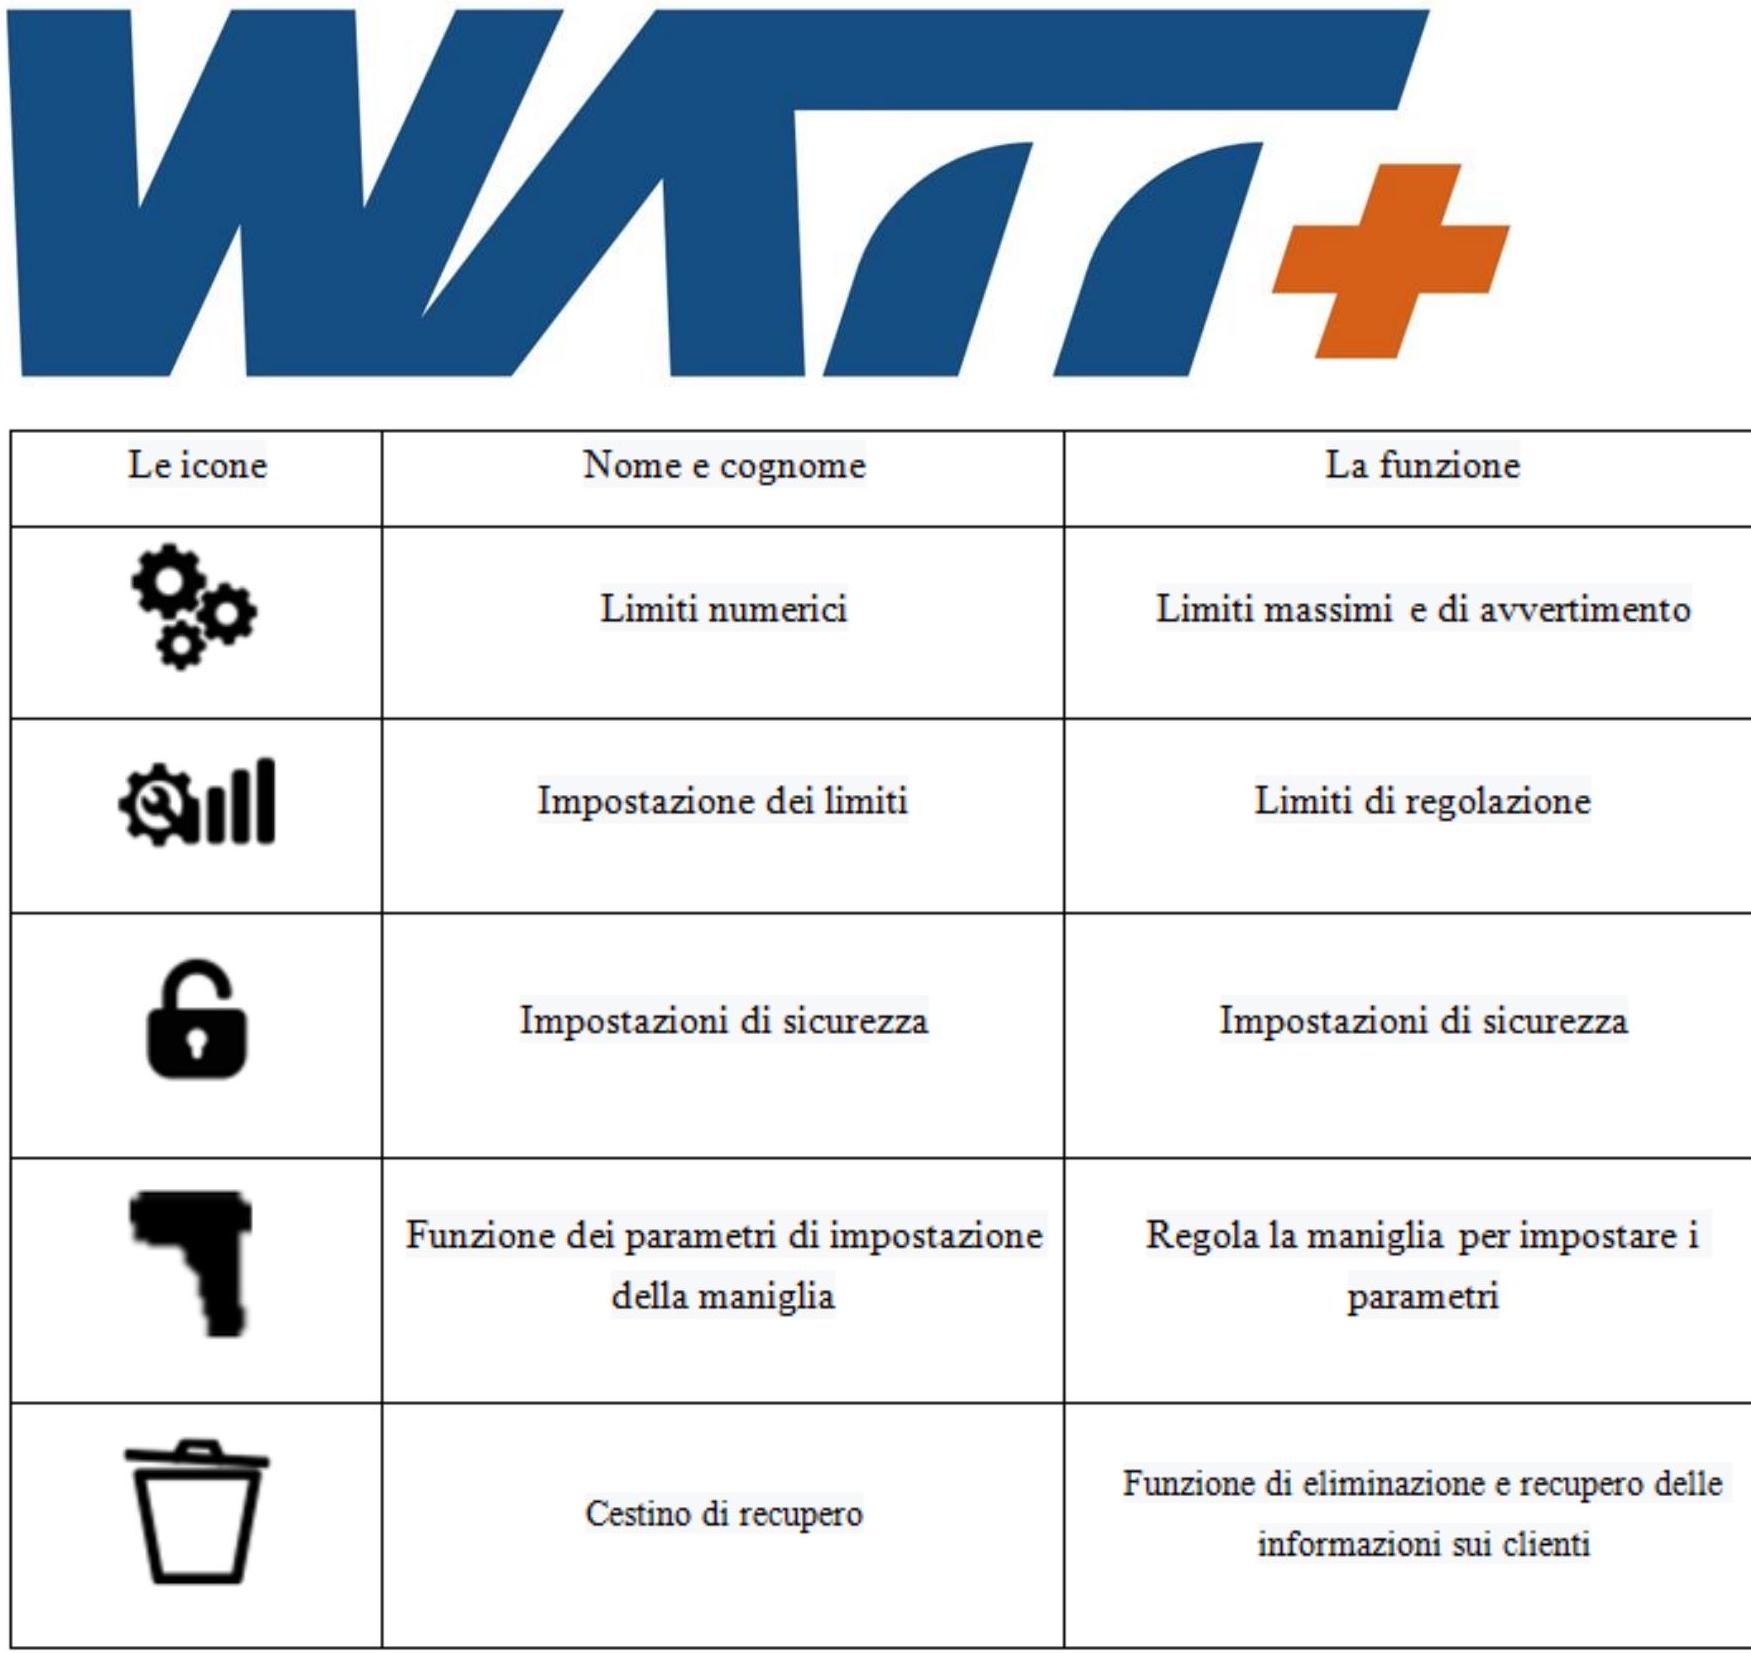
\includegraphics[alt={},max width=\textwidth]{0673f156-6613-4c24-ad16-c1dd5450a875-28_1653_1751_13_315}
\captionsetup{labelformat=empty}
\caption{4.3.1 Interfaccia back-end (processo interattivo dell'interfaccia utente delle impostazioni di modifica della password)}
\end{center}
\end{figure}

\begin{center}
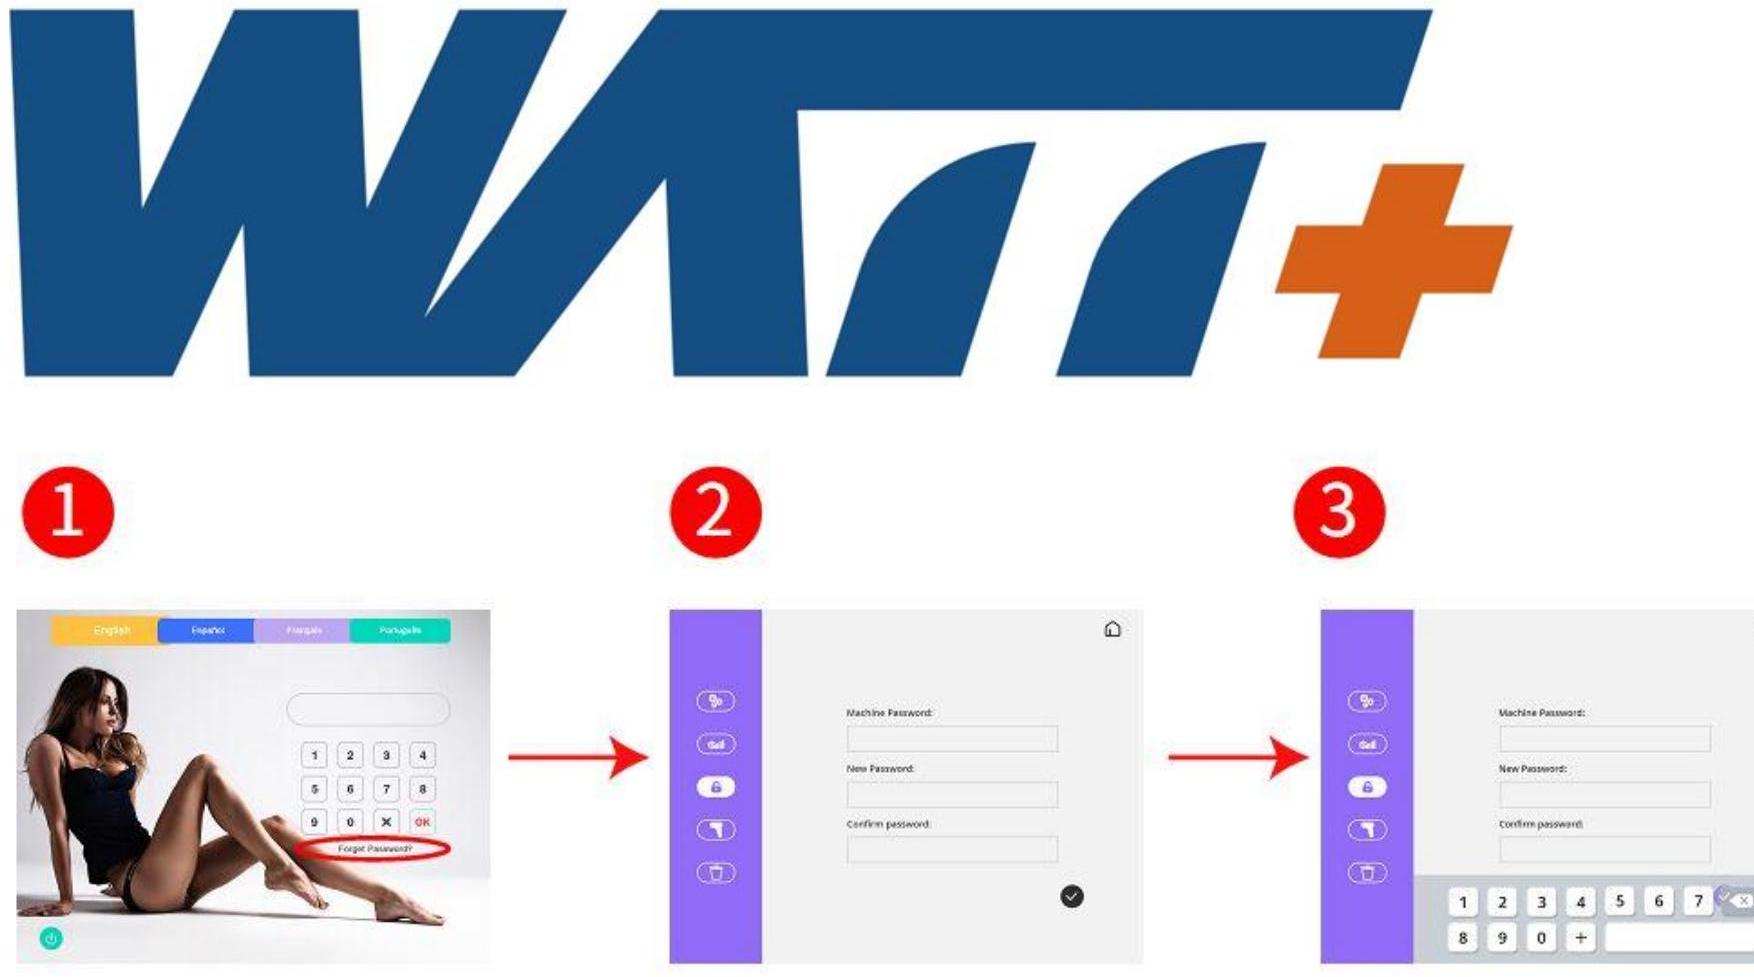
\includegraphics[max width=\textwidth, alt={}]{0673f156-6613-4c24-ad16-c1dd5450a875-29_977_1754_13_312}
\end{center}

Come mostrato nella figura, la pagina di accesso alla password, fare clic su Password dimenticata per selezionare le impostazioni di modifica della password per accedere all'interfaccia di modifica delle impostazioni di modifica della password per inserire la password da modificare.\\
4.3.2 Interfaccia in background (processo interattivo dell'interfaccia utente per il cestino della lista utenti)\\
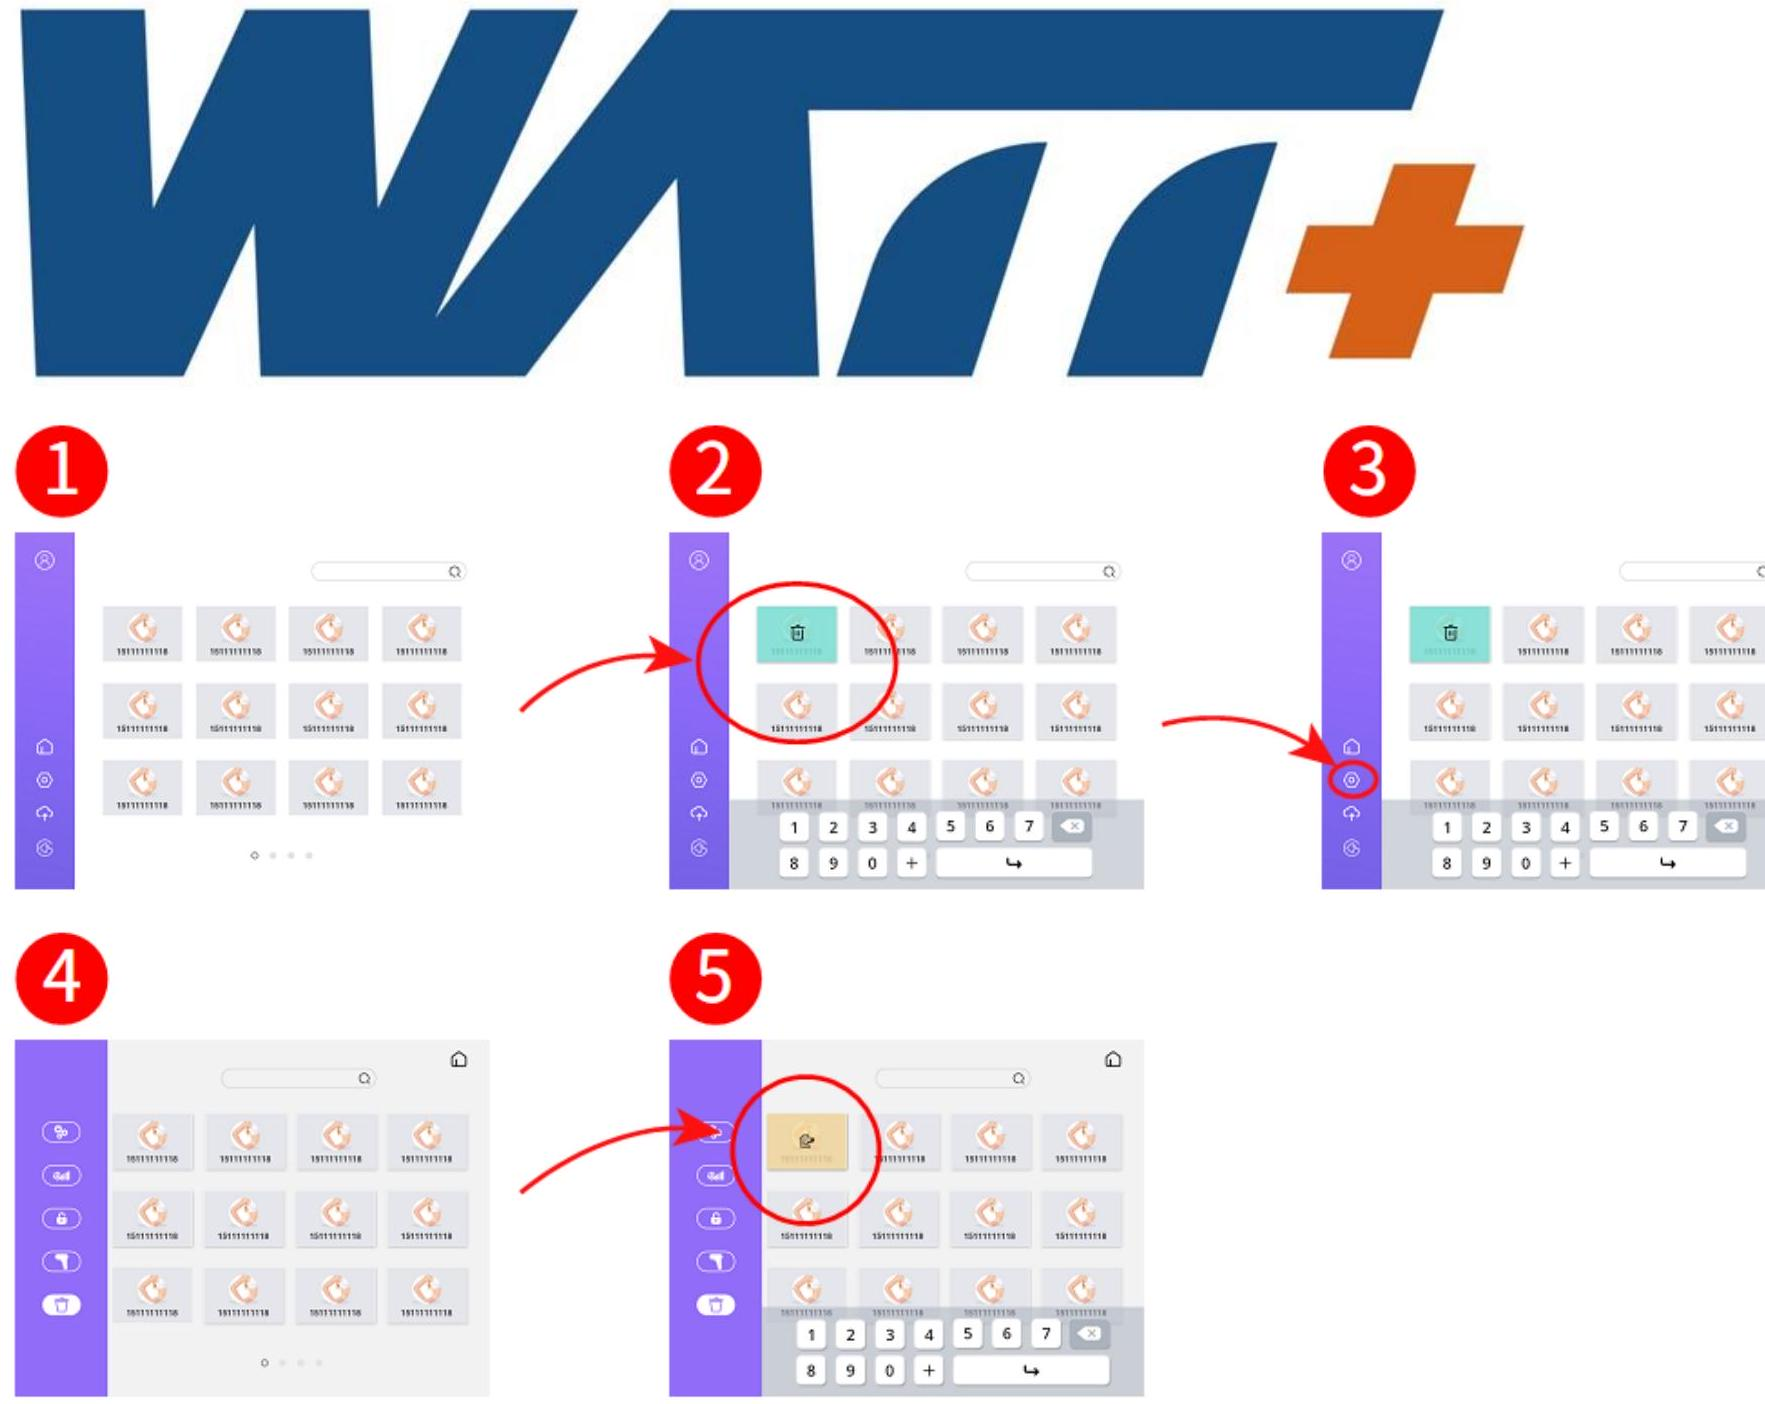
\includegraphics[max width=\textwidth, alt={}, center]{0673f156-6613-4c24-ad16-c1dd5450a875-30_1404_1765_13_301}

Come mostrato, fare clic sulla pagina dell'elenco utenti per scorrere a sinistra per visualizzare il pulsante "Elimina". Se si desidera ritirare l'eliminazione, fare clic sul pulsante Cestino a sinistra La pagina Cestino elenco utenti per scorrere a sinistra per visualizzare il pulsante Annulla eliminazione.\\
4.4 Istruzioni per l'uso del software\\
4.4.1 Come utilizzare il dispositivo

Prima del trattamento, il terapista deve comunicare dettagliatamente con il paziente.

\section{$\sqrt{1} 70+$}
Pulire la zona trattata con un detergente delicato e raderla semplicemente. E applicare un gel di raffreddamento di circa $1-2 \mathrm{~mm}$ oltre la pelle.\\
Avviare il sistema ed accedere all'interfaccia di impostazione dei parametri di trattamento;\\
Seleziona in base alla situazione reale del paziente, imposta i parametri di trattamento e fai clic sul pulsante standby/lavoro per accedere allo stato di lavoro;\\
L'indicatore della maniglia è giallo nello stato di standby, verde nello stato di preaccensione e rosso nello stato di emissione della luce.\\
Durante il processo di trattamento, l'operatore deve osservare la situazione del trattamento del paziente in tempo reale e, se necessario, regolare i parametri del trattamento in base alla situazione reale;\\
Durante il trattamento, la testa del trattamento deve evitare di rimanere a lungo nella stessa area di trattamento; Gli operatori e i pazienti devono completare le misure di protezione in tempo reale per evitare lesioni;\\
Al termine del trattamento, spegnere l'interruttore di alimentazione; Rimuovere la colla condensante dall'area di trattamento e applicarla a freddo; L'impacco freddo può essere eseguito in standby.\\
Pulire la testa del trattamento con un asciugamano caldo, quindi disinfettare la testa del trattamento con un batuffolo di cotone inumidito con un disinfettante;\\
Posizionare la testa di trattamento pulita e disinfettata nella scatola di trasporto, scollegare la spina di alimentazione dell'apparecchiatura e il processo è terminato.

\subsection{Precauzioni dopo il trattamento}
Durante il trattamento, la testa del trattamento non deve rimanere nell'area di trattamento per troppo tempo;\\
Dopo il trattamento, applicare un impacco freddo sull'area trattata per 5-10 minuti; Gli impacchi freddi possono essere eseguiti in modalità standby.\\
Per le aree di trattamento, non toccare l'acqua calda per 24 ore ed evitare il bagno in sauna e la cottura a vapore del sudore per 3-7 giorni;\\
Evitare ambienti ad alta umidità e calore elevato;\\
VILA

Evita cibi piccanti, frutti di mare e irritanti; Mangia meno verdure sensibili alla luce (come sedano, ravanello bianco, spinaci, Piatti, ecc.)\\
Prestare attenzione alla protezione solare e applicare una protezione solare con un valore SPF di $30+$. Se la luce ultravioletta è forte in estate, puoi applicare più volte, indossare un ombrellone o indossare un cappello da sole;\\
I cosmetici funzionali sono vietati per un mese nell'area di trattamento.\\
Capitolo5. Gestione dei guasti del sistema\\
5.1 Pulizia delle attrezzature

Pulire il dispositivo con un panno umido morbido, ma evitare il flusso di liquido nello strumento\\
5.2 Pulizia e sostituzione delle maniglie di movimentazione

Pulire regolarmente le lenti del manico terapeutico (una piccola quantità di particelle di pigmento schizzerà sulle lenti terapeutiche durante il trattamento, influenzando l'emissione laser), pulire le lenti terapeutiche con carta per lenti o batuffolo di cotone contenente etanolo assoluto\\
Ogni maniglia di lavorazione ha una certa durata e la testa di lavorazione deve essere sostituita circa 20 milioni di volte. In questo momento, è necessario contattare nuovamente il rivenditore per l'acquisto.

\subsection{Gestione dei guasti del sistema}
\begin{center}
\begin{tabular}{|l|l|}
\hline
Ilmalfunzionamento & MODALITÀ DI TRATTAMENTO \\
\hline
\multirow{4}{*}{Lo schermo non viene visualizzato} & Controllare il cavo di alimentazione \\
\hline
 & Controllare interruttori e fusibili \\
\hline
 & Controlla l'interruttore di alimentazione \\
\hline
 & Si prega di contattare il venditore \\
\hline
Ilpulsante di accensione non risponde & Si prega di contattare il venditore \\
\hline
\multirow{2}{*}{Inizializzazione del sistema non riuscita} & Si prega di controllare l'alimentazione \\
\hline
 & Si prega di contattare il venditore \\
\hline
\multirow{4}{*}{Emette energia laser debole o nessun laser} & La tensione è troppo bassa e la testa di elaborazione non può esser utilizzata correttamente. \\
\hline
 & Controllare la presenza di sporcizia sul riflettore laser e , in cas affermativo, pulire \\
\hline
 & Se la testa di elaborazione è danneggiata all'intemo della maniglia elaborazione, sostituire la testa di elaborazione \\
\hline
 & Rimuovere la testa di elaborazione per verificare che lo specchi anteriore non sia danneggiato \\
\hline
\end{tabular}
\end{center}

\begin{center}
\begin{tabular}{|l|l|}
\hline
\backslashbox{\begin{center}

\includegraphics[max width=\textwidth, alt={}]{0673f156-6613-4c24-ad16-c1dd5450a875-34_388_797_20_326}
\end{center}}
{
\includegraphics[max width=\textwidth, alt={}]{0673f156-6613-4c24-ad16-c1dd5450a875-34_237_467_151_1362}} &  \\
\hline
 & La testa del trattamento è surriscaldata, chiusa e raffreddata per mezz'ora dopo l'uso \\
\hline
 & Controllare la maniglia o la testa di lavorazione per eventuali perdite \\
\hline
\multirow{6}{*}{Durante il trattamento, dopo aver fatto clic sul pulsante sulla maniglia, appare un suono "cigolante"} & Controllare se la testa del trattamento laser è danneggiata e sostituirla dopo il danno \\
\hline
 & Il dispositivo non è in uso da molto tempo ed è difficile da innescare \\
\hline
 & La temperatura interna è troppo bassa per aumentare la temperatura interna \\
\hline
 & Controllare il circuito per guasti \\
\hline
 & La stanza è troppo umida, riducendo l'umidità interna \\
\hline
 & Lampada al krypton o allo xeno danneggiata, lampada \\
\hline
Temperatura del sistema di refrigerazione troppo elevata & Spegni il sistema e lascialo raffreddare per un po '. Se si verifica ancora un errore dopo il riavvio, contattare il rivenditore \\
\hline
\multirow{2}{*}{Maniglia a bassa energia} & Controllare la superficie del riflettore per impurità, pulire se necessario \\
\hline
 & Se la maniglia di manipolazione è troppo calda, spegnerla per mezz'ora prima dell'uso \\
\hline
\end{tabular}
\end{center}

\section{Capitolo 6 Specifiche}
Questo capitolo descrive i parametri di sistema più importanti e le categorie di sistema per i sistemi di trattamento.

\begin{center}
\begin{tabular}{|l|l|}
\hline
\slashbox{\quad}{\begin{tabular}{l}
T \\
$q$ \\
\end{tabular}} &  \\
\hline
I parametri & I dati relativi \\
\hline
\multicolumn{2}{|l|}{Dati di connessione elettronica} \\
\hline
Tensione di linea & $110 / 220 \mathrm{~V} \mathrm{VC} \pm 10 \%$ (vedere etichetta di sistema) \\
\hline
Frequenza della linea & $50 / 60 \mathrm{~Hz}$ \\
\hline
\multicolumn{2}{|l|}{Categorie di sistemi} \\
\hline
Protezione da scosse elettriche & Apparecchiature di prima categoria \\
\hline
Protezione dalle scosse elettriche & I Classe \\
\hline
Protezione dalle inondazioni dannose & IP65 \\
\hline
\multicolumn{2}{|l|}{Condizioni climatiche (durante il funzionamento)} \\
\hline
Temperatura ambiente & +15 C a 30 C \\
\hline
Umidità relativa & 30\%-80\% \\
\hline
Pressione atmosferica & Da $86,0 \mathrm{kPa}$ a $106,0 \mathrm{kPa}$ \\
\hline
\end{tabular}
\end{center}

Condizioni climatiche (durante lo stoccaggio grossolano durante il trasporto)

\begin{center}
\begin{tabular}{|l|l|}
\hline
Temperatura ambiente & $+5 \mathrm{Ca}+55^{\circ} \mathrm{C}$ \\
\hline
Umidità relativa & 30\%-80\% \\
\hline
Pressione atmosferica & Da $86,0 \mathrm{kPa}$ a $106,0 \mathrm{kPa}$ \\
\hline
\multicolumn{2}{|l|}{Dimensioni e pesi} \\
\hline
Dimensioni della macchina & $110 \times 50,2 \times 39 \mathrm{~cm}$ \\
\hline
Dimensione della scatola & $64 \times 47 \times 130 \mathrm{~cm}$ \\
\hline
Il Peso & 75 kg \\
\hline
\end{tabular}
\end{center}

\section*{$\sqrt{1} 60+$ }
\section{FASE A SFOLTIMENTO: 1-2 SEDUTA}
Durante la fase di sfoltimento è necessario trovare i giusti compromessi tra velocità di esecuzione e parametri. Questa fase è essenziale per garantire una prima fase di diradamento della zona trattata.

VELOCITA' DI ESECUZIONE\\
INTENSITA'\\
COLPI AL SECONDO\\
DURATA IMPULSO

Molto veloce\\
Diminuire\\
Aumentare e lavorare con Multi-spot da 6 a 8 20MS

FASE B LAVORO : 3-5 SEDUTA\\
Durante la fase di lavoro è necessario trovare i giusti compromessi tra velocità di esecuzione e parametri. Questa fase permette di creare la progressiva eliminazione dei peli indesiderati.

VELOCITA' DI ESECUZIONE\\
INTENSITA'\\
COLPI AL SECONDO\\
DURATA IMPULSO

Veloce\\
Aumentare gradualmente\\
Diminuire e lavorare con Multi-spot da 4 a 5\\
Aumentare

FASE C RIFINITURA : 6-.. SEDUTA\\
Durante la fase di rifinitura è necessario trovare i giusti compromessi tra velocità di esecuzione e parametri. Questa fase permette rifinire con precisione il lavoro svolto.

VELOCITA' DI ESECUZIONE\\
INTENSITA'\\
COLPI AL SECONDO\\
DURATA IMPULSO

Lenta\\
Aumentare\\
Diminuire e lavorare con Spot singolo\\
frazionato o multi spot da 1 a 3\\
Aumentare

\section{WARA}
\section{FASE SFOLTIMENTO}
\begin{center}
\begin{tabular}{|l|l|l|l|l|l|}
\hline
\multicolumn{2}{|c|}{\multirow{2}{*}{DA 1 A 2}} & \multicolumn{4}{|c|}{QUANTITA' PELI PRESENTI SULLA ZONA} \\
\hline
 &  & Molto Folti & Folti & Poco folti & Diradati \\
\hline
\multirow{12}{*}{
\includegraphics[max width=\textwidth, alt={}]{0673f156-6613-4c24-ad16-c1dd5450a875-38_336_35_830_370}
} &  &  &  &  &  \\
\hline
 & Sottili & \begin{tabular}{l}
34 J \\
20 MS \\
10 HZ \\
\end{tabular} & \begin{tabular}{l}
36 J \\
20 MS \\
10 HZ \\
\end{tabular} & \begin{tabular}{l}
38 J \\
20 MS \\
10 HZ \\
\end{tabular} & \begin{tabular}{l}
40 J \\
20 MS \\
10 HZ \\
\end{tabular} \\
\hline
 &  &  &  &  &  \\
\hline
 & \multirow{3}{*}{Medi} &  &  &  &  \\
\hline
 &  & \begin{tabular}{l}
31 J \\
25 MS \\
10 HZ \\
\end{tabular} & \begin{tabular}{l}
33 J \\
25 MS \\
10 HZ \\
\end{tabular} & \begin{tabular}{l}
35 J \\
25 MS \\
10 HZ \\
\end{tabular} & \begin{tabular}{l}
37 J \\
25 MS \\
10 HZ \\
\end{tabular} \\
\hline
 &  &  &  &  &  \\
\hline
 & \multirow{3}{*}{Spessi} &  &  &  &  \\
\hline
 &  & \begin{tabular}{l}
28 J \\
30 MS \\
10 HZ \\
\end{tabular} & \begin{tabular}{l}
30 J \\
30 MS \\
10 HZ \\
\end{tabular} & \begin{tabular}{l}
32 J \\
30 MS \\
10 HZ \\
\end{tabular} & \begin{tabular}{l}
34 J \\
30 MS \\
10 HZ \\
\end{tabular} \\
\hline
 &  &  &  &  &  \\
\hline
 & \multirow{3}{*}{Molto Spessi} &  &  &  & \begin{tabular}{l}
31 J \\
30 MS \\
10 HZ \\
\end{tabular} \\
\hline
 &  & \begin{tabular}{l}
25 J \\
30 MS \\
10 HZ \\
\end{tabular} & \begin{tabular}{l}
27 J \\
30 MS \\
10 HZ \\
\end{tabular} & \begin{tabular}{l}
29 J \\
30 MS \\
10 HZ \\
\end{tabular} &  \\
\hline
 &  &  &  &  &  \\
\hline
\end{tabular}
\end{center}

\section{FASE LAVORO}
\begin{center}
\begin{tabular}{|l|l|l|l|l|l|}
\hline
\multicolumn{2}{|c|}{\multirow{2}{*}{DA3A5}} & \multicolumn{4}{|c|}{QUANTITA' PELI PRESENTI SULLA ZONA} \\
\hline
 &  & Molto Folti & Folti & Poco folti & Diradati \\
\hline
\multirow{12}{*}{DIMENSIONE DEI PELI} &  &  &  &  &  \\
\hline
 & Sottili & \begin{tabular}{l}
33 J \\
65 MS \\
8 HZ \\
\end{tabular} & \begin{tabular}{l}
35 J \\
60 MS \\
8 HZ \\
\end{tabular} & \begin{tabular}{l}
37 J \\
55 MS \\
8 HZ \\
\end{tabular} &  \\
\hline
 &  &  &  &  & \begin{tabular}{l}
39 J \\
50 MS \\
8 HZ \\
\end{tabular} \\
\hline
 &  &  &  &  &  \\
\hline
 & Medi & \begin{tabular}{l}
30 J \\
75 MS \\
8 HZ \\
\end{tabular} & \begin{tabular}{l}
32 J \\
70 MS \\
8 HZ \\
\end{tabular} & \begin{tabular}{l}
34 J \\
65 MS \\
8 HZ \\
\end{tabular} & \begin{tabular}{l}
36 J \\
60 MS \\
8 HZ \\
\end{tabular} \\
\hline
 &  &  &  &  &  \\
\hline
 &  &  &  &  &  \\
\hline
 & Spessi & \begin{tabular}{l}
27 J \\
85 MS \\
8 HZ \\
\end{tabular} & \begin{tabular}{l}
29 J \\
80 MS \\
8 HZ \\
\end{tabular} & \begin{tabular}{l}
31 J \\
75 MS \\
8 HZ \\
\end{tabular} & \begin{tabular}{l}
33 J \\
70 MS \\
8 HZ \\
\end{tabular} \\
\hline
 &  &  &  &  &  \\
\hline
 &  &  &  &  &  \\
\hline
 & Molto Spessi & \begin{tabular}{l}
24 J \\
95 MS \\
8 HZ \\
\end{tabular} & \begin{tabular}{l}
26 J \\
90 MS \\
8 HZ \\
\end{tabular} & \begin{tabular}{l}
28 J \\
85 MS \\
8 HZ \\
\end{tabular} & \begin{tabular}{l}
30 J \\
80 MS \\
8 HZ \\
\end{tabular} \\
\hline
 &  &  &  &  &  \\
\hline
\end{tabular}
\end{center}

\section{WARA}
\section{FASE RIFINITURA}
\begin{center}
\begin{tabular}{|l|l|l|l|l|l|}
\hline
\multicolumn{2}{|c|}{\multirow{2}{*}{DA 6 A 8}} & \multicolumn{4}{|c|}{QUANTITA' PELI PRESENTI SULLA ZONA} \\
\hline
 &  & Molto Folti & Folti & Poco folti & Diradati \\
\hline
\multirow{12}{*}{DIMENSIONE DEI PELI} &  &  &  &  &  \\
\hline
 & Sottili & \begin{tabular}{l}
32 J \\
70 MS \\
6 HZ \\
\end{tabular} &  &  &  \\
\hline
 &  &  & \begin{tabular}{l}
34 J \\
65 MS \\
6 HZ \\
\end{tabular} & \begin{tabular}{l}
36 J \\
60 MS \\
6 HZ \\
\end{tabular} & \begin{tabular}{l}
38 J \\
55 MS \\
6 HZ \\
\end{tabular} \\
\hline
 &  &  &  &  &  \\
\hline
 & Medi & \begin{tabular}{l}
29 J \\
80 MS \\
6 HZ \\
\end{tabular} & \begin{tabular}{l}
31J \\
75 MS \\
6 HZ \\
\end{tabular} & \begin{tabular}{l}
33 J \\
70 MS \\
6 HZ \\
\end{tabular} & \begin{tabular}{l}
35 J \\
65 MS \\
6 HZ \\
\end{tabular} \\
\hline
 &  &  &  &  &  \\
\hline
 &  &  &  &  &  \\
\hline
 & Spessi & \begin{tabular}{l}
26 J \\
90 MS \\
6 HZ \\
\end{tabular} & \begin{tabular}{l}
28 J \\
85 MS \\
6 HZ \\
\end{tabular} & \begin{tabular}{l}
30 J \\
80 MS \\
6 HZ \\
\end{tabular} & \begin{tabular}{l}
32 J \\
75 MS \\
6 HZ \\
\end{tabular} \\
\hline
 &  &  &  &  &  \\
\hline
 &  &  &  &  &  \\
\hline
 & Molto Spessi & \begin{tabular}{l}
23 J \\
100 MS \\
6 HZ \\
\end{tabular} & \begin{tabular}{l}
25 J \\
95 MS \\
6 HZ \\
\end{tabular} & \begin{tabular}{l}
27 J \\
90 MS \\
6 HZ \\
\end{tabular} & \begin{tabular}{l}
29 J \\
85 MS \\
6 HZ \\
\end{tabular} \\
\hline
 &  &  &  &  &  \\
\hline
\end{tabular}
\end{center}

\begin{center}
\begin{tabular}{|l|l|l|l|l|l|}
\hline
\multicolumn{2}{|c|}{\multirow{2}{*}{DA 8 A 10}} & \multicolumn{4}{|c|}{QUANTITA' PELI PRESENTI SULLA ZONA} \\
\hline
 &  & Molto Folti & Folti & Poco folti & Diradati \\
\hline
\multirow{12}{*}{
\includegraphics[max width=\textwidth, alt={}]{0673f156-6613-4c24-ad16-c1dd5450a875-39_328_39_1704_382}
} &  &  &  &  &  \\
\hline
 & Sottili & 30 J 80 MS 5 HZ & 32 J 75 MS 5 HZ & 34 J 70 MS 5 HZ & 36 J 65 MS 5 HZ \\
\hline
 &  &  &  &  &  \\
\hline
 &  &  &  &  &  \\
\hline
 & Medi & 27 J 90 MS 5 HZ & 29 J 85 MS 5 HZ & 31 J 80 MS 5 HZ & 33 J 75 MS 5 HZ \\
\hline
 &  &  &  &  &  \\
\hline
 &  &  &  &  &  \\
\hline
 & Spessi & 24 J 100 MS 5 HZ & 26 J 95 MS 5 HZ & 28 J 90 MS 5 HZ & 30 J 85 MS 5 HZ \\
\hline
 &  &  &  &  &  \\
\hline
 &  &  &  &  &  \\
\hline
 & Molto Spessi & 21 J 100 MS 5 HZ & 23 J 95 MS 5 HZ & 25 J 90 MS 5 HZ & 27 J 85 MS 5 HZ \\
\hline
 &  &  &  &  &  \\
\hline
\end{tabular}
\end{center}

\begin{center}
\begin{tabular}{|l|l|l|l|l|l|}
\hline
\multicolumn{2}{|c|}{\multirow{2}{*}{DA 11 A 13}} & \multicolumn{4}{|c|}{QUANTITA' PELI PRESENTI SULLA ZONA} \\
\hline
 &  & Molto Folti & Folti & Poco folti & Diradati \\
\hline
\multirow{12}{*}{DIMENSIONE DEI PELI} &  &  &  &  &  \\
\hline
 & Sottili & 22 J 90 MS 4 HZ & 24 J 85 MS 4 HZ & 26 J 80 MS 4 HZ & 28 J 75 MS 4 HZ \\
\hline
 &  &  &  &  &  \\
\hline
 &  &  &  &  &  \\
\hline
 & Medi & 18 J 90 MS 4 HZ & 20 J 85 MS 4 HZ & 22 J 80 MS 4 HZ & 24 J 75 MS 4 HZ \\
\hline
 &  &  &  &  &  \\
\hline
 &  &  &  &  &  \\
\hline
 & Spessi & 14 J 120 MS 4 HZ & 16 J 100 MS 4 HZ & 18 J 100 MS 4 HZ & 20 J 100 MS 4 HZ \\
\hline
 &  &  &  &  &  \\
\hline
 &  &  &  &  &  \\
\hline
 & Molto Spessi & 10 J 120 MS 4 HZ & 12 J 100 MS 4 HZ & 14 J 100 MS 4 HZ & 16 J 100 MS 4 HZ \\
\hline
 &  &  &  &  &  \\
\hline
\end{tabular}
\end{center}

\begin{center}
\begin{tabular}{|l|l|l|l|l|l|}
\hline
\multicolumn{2}{|c|}{\multirow{2}{*}{DA 14 A 16}} & \multicolumn{4}{|c|}{QUANTITA' PELI PRESENTI SULLA ZONA} \\
\hline
 &  & Molto Folti & Folti & Poco folti & Diradati \\
\hline
\multirow{12}{*}{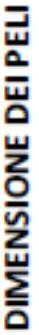
\includegraphics[max width=\textwidth, alt={}]{0673f156-6613-4c24-ad16-c1dd5450a875-40_335_39_1498_370}
} &  &  &  &  &  \\
\hline
 & Sottili & 20 J 150 MS 3 HZ & 22 J 150 MS 3 HZ & 24 J 150 MS 3 HZ & 26 J 150 MS 3 HZ \\
\hline
 &  &  &  &  &  \\
\hline
 &  &  &  &  &  \\
\hline
 & Medi & 16 J 150 MS 3 HZ & 18 J 150 MS 3 HZ & 20 J 150 MS 3 HZ & 22 J 150 MS 3 HZ \\
\hline
 &  &  &  &  &  \\
\hline
 &  &  &  &  &  \\
\hline
 & Spessi & 12 J 200 MS 3 HZ & 14 J 200 MS 3 HZ & 16 J 200 MS 3 HZ & 18 J 200 MS 3 HZ \\
\hline
 &  &  &  &  &  \\
\hline
 &  &  &  &  &  \\
\hline
 & Molto Spessi & 8 J 200 MS 3 HZ & 10 J 200 MS 3 HZ & 12 J 200 MS 3 HZ & 14 J 200 MS 3 HZ \\
\hline
 &  &  &  &  &  \\
\hline
\end{tabular}
\end{center}

What

Capitolo 7 protocolli fotobiostimolazione

\begin{center}
\begin{tabular}{|c|c|c|c|}
\hline
Potenza J & Hz & Ms & \begin{tabular}{c}
Sessioni \\
settimanali \\
\end{tabular} \\
\hline
$\mathbf{5}$ & 20 & 20 & $1 / 2$ \\
\hline
\end{tabular}
\end{center}

\section{Garanzia}
Tutti gli articoli, ove previsto, sono coperti da garanzia di legge da parte del costruttore e / o distributore\\
Fa fede la data di acquisto riportata in fattura.\\
Nel caso di acquisto da un nostro rivenditore /distributore, fa fede la data di acquisto del Rivenditore.\\
24 Mesi per articoli destinati ad uso non professionale\\
12 Mesi per articoli venduti con Partita Iva e per uso professionale\\
Non sono coperte da garanzia tutte le parti soggette ad usura od usate in modo improprio ed errato.\\
In particolare, la garanzia per il manipolo è di 12 mesi o 500.000 spot, sono escluse dalla garanzia rotture causate da caduta o negligenza da parte del cliente.\\
Le riparazioni saranno effettuate presso i centri assistenza autorizzati, o presso la nostra sede, sarà a carico del cliente la spesa di trasporto e spedizione (Franco fabbrica).\\
In caso di intervento presso la sede del cliente dovrà essere riconosciuta al servizio di assistenza il diritto di chiamata (vedere listino). Il diritto di chiamata non è dovuto entro il primo mese dopo l'acquisto) Nel periodo di garanzia verranno addebitati ai clienti\\
VILA\\
quella tipologia di interventi tecnici ritenuti a VUOTO, ove ad un intervento non si dovessero riscontrare anomalie o malfunzionamenti dovuti a negligenza e mancata manutenzione ordinaria, oppure ad una cattiva preparazione dell'operatore.\\
La garanzia decade ne seguenti casi:

\begin{itemize}
  \item Se l'apparecchiatura non ha avuto la dovuta manutenzione periodica e nel caso essa venga aperta da personale non autorizzato.
  \item collocazione, installazione e messa in opera non adeguata;
  \item utilizzo scorretto o non conforme alle prescrizioni di questo manuale;
  \item manutenzione impropria o inadeguata da parte dell'utente;
  \item funzionamento non conforme alle specifiche ambientali indicate per il prodotto;
  \item apertura non autorizzata degli involucri esterni;
  \item manomissioni e/o modifiche non autorizzate;
  \item utilizzo di accessori non originali.
\end{itemize}

Eventuali fermi apparecchiatura non danno adito a prolungamenti della garanzia e /o rimborsi per fermo macchina e quant' altro.

\begin{itemize}
  \item Sostituire l'acqua OGNI 3 MESI, pena la decadenza della garanzia.
  \item Sostituzione filtri: ogni 6 mesi entrambi i filtri. pena la decadenza della garanzia.
  \item Utilizzare solo ricambi originali, pena la decadenza della garanzia.
\end{itemize}

\section{CONSENSO INFORMATO PER TRATTAMENTO CON LASER PER EPILAZIONE}
Io sottoscritto/a nato/a il

\begin{center}
\begin{tabular}{lllll}
Residente in Via/Piazza &  & Cap &  & Città \\
Cod. Fiscale & Pr &  &  &  \\
Tel/Cell &  &  & E-mail &  \\
Colore capelli $\square$ Biondo & $\square$ Castano & $\square$ Rosso & $\square$ Nero & $\square$ Altro \\
\end{tabular}
\end{center}

Nel caso di minore:\\
Nome e Cognome (del minore)\\
Documento numero\\
□ Autorizzo e accetto lo svolgimento del trattamento da me richiesto al minore di cui sopra, assumendone tutte le responsabilità\\
DESCRIZIONE TRATTAMENTO\\
L'epilazione laser è una tecnica che permette la rimozione dei peli superflui su viso e corpo attraverso la foto termolisi (ossia l'energia luminosa che si trasforma in calore) provoca la distruzione del bulbo e delle cellule che lo rigenerano, consentendo di ottenere risultati duraturi. Lo scopo finale è quello di provocare, seduta dopo seduta, un progressivo assottigliamento e diradamento della peluria, rallentandone fortemente la ricrescita e rendendola non visibile ad occhio nudo.

\section{$\sqrt{1} \times 1+$}
Tale trattamento elimina i peli in fase di crescita, denominata Anagen, e dal momento che nell'uomo i cicli vitali dei peli non sono sincronizzati, per ottenere una riduzione dei peli ( $60-80 \%$ ) del patrimonio pilifero sono necessarie più sedute di epilazione. Comunque, la crescita dei peli è soggettiva e in particolare i soggetti con disfunzioni endocrine anche lievi, irsutismo, ipertricosi, sottoposti a cure cortisoniche ed ormonali, o con habitus ansioso-depressivo, potranno avere la ricrescita o la comparsa di nuovi peli. Di conseguenza, anche se questo trattamento è efficace nella maggior parte delle persone, non vi può essere a priori nessuna garanzia di efficacia per ciascun cliente. I risultati individuali dipendono, infatti, da una serie di fattori, tra cui età, tipo di pelle, caratteristiche dei peli e assetto ormonale.\\
INDICAZIONI ED EFFETTI COLLATERALI

\begin{itemize}
  \item Sono possibili modesti effetti collaterali quali micro ustioni, arrossamenti, vesciche, ipo o iperpigmentazioni.
  \item II/La cliente dovrà depilarsi 2 giorni prima della seduta (Usare il metodo indicato della tecnica). II/La cliente non deve assolutamente utilizzare cerette, rasoio, pinzette o altri metodi di depilazione durante e successivamente al percorso del trattamento, rischia la perdita parziale o anche totale del risultato.
  \item Prima e Dopo la seduta di epilazione laser è importante evitare l'esposizione al sole o lampade abbronzante negli ultimi 15 giorni, in quanto la pelle risulta particolarmente vulnerabile agli effetti delle radiazioni ultraviolette e può reagire creandone macchie e/o ustioni. Sulle zone trattate esposte alla luce del sole come, ad esempio, il viso è consigliabile usare, quindi, un filtro con protezione alta (SPF 50), anche in inverno.
  \item Dopo aver realizzato la foto epilazione è consigliabile applicare sulla zona trattata i cosmetici indicati dell'operatore, seguire tutti i consigli ed utilizzare i filtri solare, per evitare alterazioni della pigmentazione e macchie solari.
  \item L'epilazione laser non è indicata a chi ha poco contrasto tra peluria e carnagione (peli chiari su pelle chiara; peli medio-scuri su carnagione scura ecc.), considerati i rischi di depigmentazione cutanea.\\
What
\end{itemize}

Ps. In caso di dubbi è sempre meglio chiedere consiglio al proprio medico di base o rivolgersi ad un dermatologo

\section{POST TRATTAMENTO POSSONO VERIFICARSI:}
\begin{itemize}
  \item Arrossamento: è normale che l'area trattata assuma un aspetto rosato (Eritema) o decisamente rossastro, a seconda della sensibilità di ogni individuo, destinato a ridursi spontaneamente in pochi giorni. (Utilizzare i prodotti indicati della tecnica).
  \item Discromie: la pelle potrebbe assumere un colorito più scuro o meno intenso (iperpigmentazioni, ipopigmentazioni).
  \item Cicatrici: anche se molto raramente, la pelle può guarire con aspetto cicatriziale.
\end{itemize}

\section{CONTROINDICAZIONI:}
Herpes Simplex, Pregressa radioterapia o Chemioterapia, Terapie in atto controindicate(Corticosteroidei, Antibiotici, Trattamenti ormonali sostitutivi, Farmaci immunosoppressori e Fotosensibilizzanti (come l'isotretinoina per l'acne), Malattie autoimmunitarie, Fototipi elevati (IV-VI Fitzpatrick), Nei, Tatuaggi nella zona da trattare, Gravidanza, Allattamento, Portatore di pacemaker, Cardiopatia, Dispositivo per incontinenza, Pompa Insulinica, In Regime di Steroidi, Pillola antifecondativa (in rari casi macchia la pelle), Emofiliasi, Eczema, Ferite aperte, Psoriasi, Naevus Pilous (neo con peli), Diabete, Patologie della pelle, Neoplasie, Escoriazioni ed abrasioni, Epilessia, Asma, Pelle abbronzata.

\section{INFORMAZIONI GENERALI}
Ho avuto modo di discutere in maniera adeguata ed esauriente le caratteristiche del trattamento in questione con che mi ha esposto in termini a me pienamente comprensibili le tecniche attualmente disponibili per l'effettuazione del trattamento da me desiderato. Mi è stato inoltre adeguatamente spiegato che il beneficio atteso da tale trattamento si raggiunge con più

\section{$\sqrt{1} 70+$}
sedute, la durata del trattamento di foto epilazione dipende dal singolo individuo (soggettivo), e della zona del corpo da trattare. Indicativamente si ipotizza circa dalle 7 alle 10 sedute come programma, e si effettua una seduta ogni 4 settimana circa. Anche se si può rendere necessaria qualche seduta come mantenimento. Mi è stato illustrato in modo completo che in taluni casi il risultato può essere insoddisfacente per una buona risposta individuale, indipendente dal trattamento. In questi casi non può essere richiesto rimborso. Ho avuto quindi ampia e dettagliata spiegazione sul procedimento, rischi, effetti collaterali. Sono cosciente ed accetto che se interrompo il ciclo di sedute di mia spontanea volontà, per gravidanza o per malattia non potrò richiedere il rimborso delle sedute effettuate né all'operatore né al centro estetico. Mi è stata data ampia spiegazione dei comportamenti e precauzioni da tenere prima e dopo il trattamento laser, in particolare della necessità di non esporsi al sole o a raggi ultravioletti prima e dopo il trattamento. Sono consapevole che il mancato rispetto da parte mia delle istruzioni avute e del procedimento corretto dei trattamenti potrebbe compromettere il risultato del trattamento stesso. Il mancato compimento delle sessioni sono di mia responsabilità, liberando l'operatore da qualsiasi responsabilità sul risultato. Con questa dichiarazione, quindi, dopo aver compreso tutte le informazioni sopra elencate che mi sono state esposte esaurientemente e comprensibilmente chiedo di essere sottoposto al trattamento Laser. lo sottoscritto/a dichiaro di aver letto attentamente il foglio informativo allegato e dichiaro il mio consenso a sottopormi al trattamento con il Laser. Tutela della Privacy

Tutti i dati personali sopra riportati verranno trattati in osservazione del Regolamento (UE) n. 2016/679.\\
Rivolgersi al personale per richiedere il regolamento privacy completo.\\
Data ....../....../.....

Firma del\\
Cliente

\section{TECNOLOGIA:}
UDI 06973663791049 FABBRICANTE CN-MF-000019748

\section{Modelo: ALPHA LASER}
\section{Número de serie: ..R....../.......}
La verifica è stata effettuata nell'ambito seguente:\\
Informazioni sulla Dichiarazione di Conformità:\\
Risultato: Legislazione: Standard:\\[0pt]
✓ Direttiva LVD [2014/35/UE] EN 60335-

1:2012+A11:2014+A13:2017+A1:2019+A14:2019+A2:2019+A15:2021\\
EN IEC 60335-2-115:2023+A11:2023\\
EN 62233:2008\\[0pt]
✓ Compatibilità elettromagnetica (EMC) [2014/30/UE] EN IEC 55014-1:2021

EN IEC 61000-3-2:2019+A1:2021\\
EN 61000-3-3:2013+A1:2019+A2:2021\\
EN IEC 55014-2:2021

Il processo di valutazione è stato svolto in conformità alle regole.\\
1639\\
c $\epsilon$\\
Data di emissione: 16.09.2024\\
Data di scadenza: 16.09.2029\\
Madrid 16.09.24

\section*{W $/ \sqrt{6+}$ }
\section{RESPONSABILE E/O DIRETTORE TECNICO}
\section{CENTRO ESTETICO}
\section*{Il responsabile tecnico è il professionista che si occupa della supervisione del lavoro di un team che, all'interno di un'azienda. }
\section{TECNOLOGIA LASER}
\section{Firma}
\section{Allegato Sicurezza LASER}
L'utilizzatore viene informato dei rischi che l'utilizzo delle apparecchiature ad alta tecnologia possono comportare es. rischi ottici, elettrici, incendio e biologici e si assume la responsabilità di operare in base alle leggi vigenti nel paese d'utilizzo e di operare in piena sicurezza osservando le indicazioni del manuale d'uso, tenendo inoltre presente le regole dell'istituto dettate dalle norme sulla sicurezza interna, norme antincendio e norme sulla prevenzione degli incidenti sul lavoro. Quest'apparecchiatura è stata progettata con un sistema di diagnostica che non permette l'utilizzo dell'apparecchiatura in caso di anomalie tecniche. Considerando l'alta intensità e l'alta energia di uscita del laser durante il funzionamento, tutto il personale interessato deve rispettare le misure precauzionali. Prima di procedere all'utilizzo dell'apparecchiature verificarne l'esatta installazione e verificare tutti i suoi accessori. • Controllare che l'alimentazione di rete sia quella corretta • Verificare la messa a terra dell'impianto • Non collegare l'apparecchiatura a ciabatte o prese multiple • Utilizzare prese di corrente collegate direttamente al quadro elettrico • Non installare le apparecchiature in luoghi con alta umidità • Verificare che non ci siano perdite di liquidi di raffreddamento • Controllare la dotazione di sicurezza (occhialini) che deve essere conforme alle specifiche tecniche • Controllare le diverse connessioni e che non appaiano guaine usurate o fili scoperti • Anche se munito di ruote e viste le notevoli dimensioni e peso, utilizzare la massima attenzione negli spostamenti dell'apparecchiatura • Quando non si utilizza l'apparecchiatura, scollegare dalla rete o posizionare il tasto accensione in OFF • Nelle aree di utilizzo dell'apparecchiatura deve essere posizionato in un luogo visibile un cartello con precise indicazioni relative al particolare danno biologico indotto (depilazione permanente) e uno per Radiazioni Laser.

È responsabilità di chi detiene la titolarità dell'attività di estetista/Studio medico: • mantenere controlli di sicurezza (specifici per l'apparecchiatura laser); • fornire addestramento ad eventuale altro personale che utilizza (e collabora all'utilizzo) l'apparecchiatura laser; • fornire informazioni (specifiche per l'apparecchiatura laser) a coloro che ricevono il trattamento estetico e ad ogni altro visitatore. • Compilare e far firmare il consenso informato. Il trattamento deve essere effettuato da operatori estetici che abbiano ricevuto dal costruttore o da altro ente competente adeguata formazione sia per gli aspetti di sicurezza (richiamati peraltro dal manuale d'uso) sia per gli aspetti "tecnici" dei trattamenti stessi. Controlli, informazioni e modalità di addestramento specifici per l'apparecchiatura laser dipendono dalla classe del laser e sono da richiedere direttamente al costruttore/fornitore dell'apparecchiatura laser, come esplicitate in modo chiaro nel presente manuale d'uso. Chi utilizza un'apparecchiatura laser deve conoscere il significato: - delle classi laser; - dell'intero contenuto delle etichette di avvertimento dell'apparecchiatura laser; - dei rischi all'occhio e alla pelle dei diversi tipi di laser; - delle possibili interazioni del laser con oggetti nell'ambiente circostante; - di efficacia delle protezioni oculari. 2.3 Classificazione dei rischi da laser Laser è l'acronimo di Light Amplification by Stimulated Emission of Radiation (Amplificazione della Luce attraverso un'Emissione Stimolata di Radiazioni). Il laser produce un intenso fascio di luce\\
altamente direzionale. L'esposizione di alcuni tipi di laser può provocare danni al corpo umano in particolar modo agli occhi e alla pelle. Sono state effettuate numerose ricerche sui danni agli occhi e alla pelle dovuti da esposizione da radiazioni laser per capirne i rischi. Ora è ampiamente dimostrato che l'occhio umano è molto più vulnerabile rispetto alla pelle. Per regolarsi sulla sicurezza di un laser, il centro CDRH, Center for Devices \& Radiological Health (Centro per i Dispositivi \& Salute Radiologica), ha classificato i laser in diverse categorie basate sulla forza d'uscita e sulla lunghezza dell'onda. Classe 1: La classe laser 1 è considerata dalla attuale conoscenza medica sicura. Questa classe include tutti i laser o sistemi laser che non possono emettere livelli di radiazioni ottiche al di sopra dei limiti di esposizione per l’occhio umano sotto qualsiasi condizione di esposizione inerenti al design del prodotto laser. Ci può essere un laser più dannoso nella classe 1 ma comunque nessuna radiazione potrà mai fuoriuscire. Classe 2: Questi laser non possono causare danni agli occhi in circostanze normali, possono provocare danni solo se a contatto con gli occhi per un lungo periodo di tempo. La classe 2 dei laser opera solo nel range visibile $(400-700 \mathrm{~nm})$ e ha un potere di uscita uguale o inferiore di 1 mW . Class 3a: La classe laser 3a non può causare danni all'occhio durante il periodo del lampeggio. Comunque l'infortunio è possibile se il fascio è visto attraverso un binocolo o simili dispositivi ottici o fissando direttamente il fascio. La Potenza output per Onde Continue(CW Continue Wave) laser operante nel campo visibile è compresa tra $1-5 \mathrm{~mW}$. Classe 3b: La classe laser 3b può produrre infortuni accidentali agli occhi attraverso l'esposizione diretta del laser nell'occhio o attraverso immagini riflesse nell'occhio. La potenza output della classe laser 3b è compresa tra $5-$ 500 mW per laser CW. Classe 4: Un qualsiasi laser o un sistema laser di categoria 4 eccede nei limiti di output (Limiti di Emissioni Accettabili AEL) nella quale rientra la classe 3. Per cui questi laser quindi possono rappresentare un pericolo per la pelle, bruciature o un danno per riflessione diffuso. Sono richieste quindi misure di controllo elevate per i laser o i sistemi laser di categoria 4. Classificazione internazionale La Commissione elettrotecnica internazionale (IEC) è un'organizzazione globale che prepara e pubblica gli standard internazionali per tutti elettrici, tecnologie elettroniche e correlate. Il documento IEC 60825-1 è la norma primaria che delinea la sicurezza dei prodotti laser. La classificazione si basa su calcoli e determinato dal Accessible Emission Limit (AEL) come con lo standard ANSI, ma lo standard IEC incorpora anche la visualizzazione condizioni: Classe 1: Laser che sono sicuri nelle condizioni di funzionamento ragionevolmente prevedibili, incluso l'uso di strumenti oCici per la visione del fascio. Classe 1M: Laser che emettono nell'intervallo di lunghezza d'onda tra $302,5 \mathrm{nrn}$ e 4000 nrn che sono sicuri nelle condizioni di funzionamento ragionevolmente prevedibili, ma possono essere pericolosi se l'operatore impiega ottiche di osservazione all'interno del fascio. Class 2: Laser che emettono radiazione visibile nell'intervallo di lunghezze d'onda tra 400 e 700 nrn ; la protezione dell'occhio è normalmente assicurata dalle reazioni di difesa compreso il riflesso palpebrale. Questa reazione fornisce un'adeguata protezione nelle condizioni di funzionamento ragionevolmente prevedibili, incluso l'uso di strumenti ottici per la visione del fascio. Classe 2 M : Laser che emettono radiazione visibile nell'intervallo di lunghezze d'onda tra 400 e 700 nrn ; la protezione dell'occhio è normalmente assicurata dalle reazioni di difesa compreso il riflesso palpebrale; comunque, la visione del fascio può essere più pericolosa se l'operatore impiega ottiche\\
di osservazione all'interno del fascio. Classe 3R: Laser che emettono nell'intervallo di lunghezze d'onda tra 302,5 e 106nrn, dove la visione diretta del fascio è potenzialmente pericolosa ma il rischio è più basso dei laser di Classe 3B; i requisiti del costruttore e le misure di controllo per il Responsabile delle attività sono meno che per i laser di Classe 3B. Il LEA è inferiore a cinque volte il LEA di Classe 2 nell'intervallo di lunghezze d'onda tra 400 e 700 nrn , ed inferiore a cinque volte il LEA di Classe 1 per le altre lunghezze d'onda. Classe 3B: Laser che sono normalmente pericolosi nel caso di esposizione diretta del fascio; la visione della radiazione diffusa è normalmente non pericolosa. Classe 4: Laser che sono anche in grado di produrre riflessioni diffuse pericolose; Possono causare lesioni alla pelle e potrebbero anche costituire un pericolo d'incendio. Il loro uso richiede un'estrema cautela. $\_\_\_\_$

\section{Pericoli oculari}
È obbligatorio proteggere gli occhi sia dell'operatore che del cliente L'apparecchiatura è un laser di classe 4, la più pericolosa per il sistema oculare, pertanto la radiazione sia diretta che diffusa può provocare seri danni all'apparato visivo. Il corretto uso fa riferimento alla normativa EN 60825-1 sulla corretta protezione dalle emissioni laser pericolose. Seguire sempre le indicazioni per una buona protezione sia del personale che della clientela. Si consiglia di utilizzare l'apparecchiatura in locali privi di pareti e superfici riflettenti. Utilizzare sempre gli occhiali di protezione per tutte le persone che sostano all'interno di essa. Eleggere una persona di riferimento all'interno dell'istituto che abbini la sicurezza, il monitoraggio delle informazioni acquisite sia tecniche che della clientela. Consigli per la sicurezza oculare: • Non guardare mai direttamente l'emettitore • Indossare sempre occhiali di protezione, sotto i quali disporre del cotone per una maggior protezione oculare della cliente. • Indicare sempre con un cartello od un segnale luminoso la presenza di trattamento in cabina o in studio • Indicare con cartelli la presenza di emissioni laser sia all'ingresso della stanza che nella stanza stessa • Utilizzare occhiali protettivi di classe IV con lunghezza ottica di almeno 5 o superiore alla lunghezza d'onda di 800-830 • Durante il trattamento l'operatore deve mantenere una distanza di sicurezza dall'emettitore quantificabile in almeno 40 cm • Per ogni singolo operatore distribuire i trattamenti nell'arco della giornata o alternare diversi operatori • Anche se si indossano gli occhiali di protezione non guardare mai l'emettitore laser • Non guardare direttamente il laser o la luce riflessa • Eliminare specchi e/o parti riflettenti (ad esempio in acciaio) • Togliere orologi, bracciali e tutti gli oggetti che hanno potere riflettente • Attenersi sempre alle procedure di sicurezza • Evitare di dirigere il fascio laser altrove se non verso la zona da trattare. • Non trattare sopracciglia, ciglia o zone limitrofe alla zona oculare • La sosta di persone all'interno della stanza dove si effettuano i trattamenti deve limitarsi al personale addetto ed al paziente / cliente • Controllare l'integrità del manipolo e verificare che in esso non ci siano lesioni che possano permettere alla luce laser di disperdersi nell'ambiente. • È fatto obbligo il non utilizzo di cellulari all'interno della cabina. La non osservanza delle condizioni di sicurezza può provocare gravi danni all’ apparato visivo.

Quest'apparecchiatura è stata progettata con un sistema di diagnostica che non permette l'utilizzo dell'apparecchiatura in caso di anomalie tecniche.\\
Considerando l'alta intensità e l'alta energia di uscita del laser durante il funzionamento, tutto il personale interessato deve rispettare le misure precauzionali.\\
Prima di procedere all'utilizzo dell'apparecchiature verificarne l'esatta installazione e verificare tutti i suoi accessori.

\begin{itemize}
  \item Controllare che l'alimentazione di rete sia quella corretta
  \item Verificare la messa a terra dell'impianto
  \item Non collegare l'apparecchiatura a ciabatte o prese multiple
  \item Utilizzare prese di corrente collegate direttamente al quadro elettrico
  \item Non installare le apparecchiature in luoghi con alta umidità
  \item Verificare che non ci siano perdite di liquidi di raffreddamento
  \item Controllare la dotazione di sicurezza (occhialini) che deve essere conforme alle specifiche tecniche
  \item Controllare le diverse connessioni e che non appaiano guaine usurate o fili scoperti
  \item Anche se munito di ruote e viste le notevoli dimensioni e peso, utilizzare la massima attenzione negli spostamenti dell'apparecchiatura, utilizzare sempre il freno a ruota.
  \item Quando non si utilizza l'apparecchiatura, scollegare dalla rete o posizionare il tasto accensione in OFF
  \item Nelle aree di utilizzo dell'apparecchiatura deve essere posizionato in un luogo visibile un cartello con precise indicazioni relative al particolare danno biologico indotto (depilazione permanente o semi permanente o progressivamente permanente).
\end{itemize}

\section{È responsabilità di chi detiene la titolarità dell'attività di estetista:}
\begin{itemize}
  \item mantenere controlli di sicurezza ove richiesto Responsabile di sicurezza RSPP (specifici per l'apparecchiatura laser);
  \item fornire addestramento ad eventuale altro personale che utilizza (e collabora all'utilizzo) l'apparecchiatura laser;
  \item fornire informazioni (specifiche per l'apparecchiatura laser) a coloro che ricevono il trattamento estetico e ad ogni altro visitatore.\\
Controlli, informazioni e modalità di addestramento specifici per l'apparecchiatura laser dipendono dalla classe del laser e sono da richiedere direttamente al costruttore/fornitore dell'apparecchiatura laser, come esplicitate in modo chiaro nel presente manuale d'uso.
\end{itemize}

\section{Chi utilizza un'apparecchiatura laser deve conoscere il significato:}
\begin{itemize}
  \item delle classi laser;
  \item dell'intero contenuto delle etichette di avvertimento dell'apparecchiatura laser;
  \item dei rischi all'occhio e alla pelle dei diversi tipi di laser;
  \item delle possibili interazioni del laser con oggetti nell'ambiente circostante;
  \item di efficacia delle protezioni oculari e dell'efficacia del trattamento utilizzando apparecchiature laser.
\end{itemize}

\section{Classificazione dei rischi da laser}
Laser è l'acronimo di Light Amplification by Stimulated Emission of Radiation (Amplificazione della Luce attraverso un'Emissione Stimolata di Radiazioni). Il laser produce un intenso fascio di luce altamente direzionale. L'esposizione di alcuni tipi di laser può provocare danni al corpo umano in particolar modo agli occhi e alla pelle. Sono state effettuate numerose ricerche sui danni agli occhi e alla pelle dovuti da esposizione da radiazioni laser per capirne i rischi. Ora è ampiamente dimostrato che l'occhio umano è molto più vulnerabile rispetto alla pelle.

Per regolarsi sulla sicurezza di un laser, il centro CDRH, Center for Devices \& Radiological Health (Centro per i Dispositivi \& Salute Radiologica), ha classificato i laser in diverse categorie basate sulla forza d'uscita e sulla lunghezza dell'onda.

Classe 1: La classe laser 1 è considerata dalla attuale conoscenza medica sicura. Questa classe include tutti i laser o sistemi laser che non possono emettere livelli di radiazioni ottiche al di sopra dei limiti di esposizione per l'occhio umano sotto qualsiasi condizione di esposizione inerenti al design del prodotto laser. Ci può essere un laser più dannoso nella classe 1 ma comunque nessuna radiazione potrà mai fuoriuscire.

Classe 2: Questi laser non possono causare danni agli occhi in circostanze normali, possono provocare danni solo se a contatto con gli occhi per un lungo periodo di tempo. La classe 2 dei laser opera solo nel range visibile ( $400-700 \mathrm{~nm}$ ) e ha un potere di uscita uguale o inferiore di 1 mW .\\
Class 3a: La classe laser 3a non può causare danni all'occhio durante il periodo del lampeggio. Comunque l'infortunio è possibile se il fascio è visto attraverso un binocolo o simili dispositivi ottici o fissando direttamente il fascio. La Potenza output per Onde Continue(CW - Continue Wave) laser operante nel campo visibile è compresa tra $1-5 \mathrm{~mW}$.\\
Classe 3b: La classe laser 3b può produrre infortuni accidentali agli occhi attraverso l'esposizione diretta del laser nell'occhio o attraverso immagini riflesse nell'occhio. La potenza output della classe laser 3b è compresa tra $5-500 \mathrm{~mW}$ per laser CW .\\
Classe 4: Un qualsiasi laser o un sistema laser di categoria 4 eccede nei limiti di output (Limiti di Emissioni Accettabili AEL) nella quale rientra la classe 3. Per cui questi laser quindi possono rappresentare un pericolo per la pelle, bruciature o un danno per riflessione diffuso. Sono richieste quindi misure di controllo elevate per i laser o i sistemi laser di categoria 4.

\section{Classificazione internazionale}
La Commissione elettrotecnica internazionale (IEC) è un'organizzazione globale che prepara e pubblica gli standard internazionali per tutti elettrici, tecnologie elettroniche e correlate. Il documento IEC 60825-1 è la norma primaria che delinea la sicurezza dei prodotti laser. La classificazione si basa su calcoli e determinato dal Accessible Emission Limit (AEL) come con lo standard ANSI, ma lo standard IEC incorpora anche la visualizzazione condizioni:

Classe 1: Laser che sono sicuri nelle condizioni di funzionamento ragionevolmente prevedibili, incluso l'uso di strumenti oCici per la visione del fascio.\\
Classe 1M: Laser che emettono nell'intervallo di lunghezza d'onda tra $302,5 \mathrm{nrn}$ e 4000 nrn che sono sicuri nelle condizioni di funzionamento ragionevolmente prevedibili, ma possono essere pericolosi se l'operatore impiega ottiche di osservazione all'interno del fascio.\\
Class 2: Laser che emettono radiazione visibile nell'intervallo di lunghezze d'onda tra 400 e 700 nrn ; la protezione dell'occhio è normalmente assicurata dalle reazioni di difesa compreso il riflesso palpebrale. Questa reazione fornisce un'adeguata protezione nelle condizioni di funzionamento ragionevolmente prevedibili, incluso l'uso di strumenti ottici per la visione del fascio.\\
Classe 2M: Laser che emettono radiazione visibile nell'intervallo di lunghezze d'onda tra 400 e 700 nrn ; la protezione dell'occhio è normalmente assicurata dalle reazioni di difesa compreso il riflesso palpebrale; comunque, la visione del fascio può essere più pericolosa se l'operatore impiega ottiche di osservazione all'interno del fascio.

Classe 3R: Laser che emettono nell'intervallo di lunghezze d'onda tra 302,5 e 106 nrn , dove la visione diretta del fascio è potenzialmente pericolosa ma il rischio è più basso dei laser di Classe 3B; i requisiti del costruttore e le misure di controllo per il Responsabile delle attività sono meno che per i laser di Classe 3B. Il LEA è inferiore a cinque volte il LEA di Classe 2 nell'intervallo di lunghezze d'onda tra 400 e 700 nrn, ed inferiore a cinque volte il LEA di Classe 1 per le altre lunghezze d'onda.\\
Classe 3B: Laser che sono normalmente pericolosi nel caso di esposizione diretta del fascio; la visione della radiazione diffusa è normalmente non pericolosa.\\
Classe 4: Laser che sono anche in grado di produrre riflessioni diffuse pericolose; Possono causare lesioni alla pelle e potrebbero anche costituire un pericolo d'incendio. Il loro uso richiede un'estrema cautela.

\section{È obbligatorio proteggere gli occhi sia dell'operatore che del cliente}
L'apparecchiatura è un laser di classe 4, la più pericolosa per il sistema oculare, pertanto la radiazione sia diretta che diffusa può provocare seri danni all’apparato visivo.\\
Il corretto uso fa riferimento alla normativa EN 60825-1 sulla corretta protezione dalle emissioni laser pericolose.\\
Seguire sempre le indicazioni per una buona protezione sia del personale che della clientela.\\
Si consiglia di utilizzare l'apparecchiatura in locali privi di pareti e superfici riflettenti.\\
Utilizzare sempre gli occhiali di protezione per tutte le persone che sostano all'interno di essa. Eleggere una persona di riferimento all'interno dell'istituto che abbini la sicurezza, il monitoraggio delle informazioni acquisite sia tecniche che della clientela.

Consigli per la sicurezza oculare:

\begin{itemize}
  \item Non guardare mai direttamente l'emettitore
  \item Indossare sempre occhiali di protezione, sotto i quali disporre del cotone per una maggior protezione oculare della cliente.
  \item Indicare sempre con un cartello od un segnale luminoso la presenza di trattamento in cabina o in studio
  \item Indicare con cartelli la presenza di emissioni laser sia all'ingresso della stanza che nella stanza stessa
  \item Utilizzare occhiali protettivi di classe IV con lunghezza ottica di almeno 5 o superiore alla lunghezza d'onda di 790-830 (ATTENZIONE A QUELLO CHE SI TROVA IN COMMERCIO)
  \item Durante il trattamento l'operatore deve mantenere una distanza di sicurezza dall'emettitore quantificabile in almeno 40 cm
  \item Per ogni singolo operatore distribuire i trattamenti nell'arco della giornata o alternare diversi operatori
  \item Anche se si indossano gli occhiali di protezione non guardare mai l'emettitore laser
  \item Non guardare direttamente il laser o la luce riflessa
  \item Eliminare specchi e/o parti riflettenti (ad esempio in acciaio)
  \item Togliere orologi, bracciali e tutti gli oggetti che hanno potere riflettente
  \item Attenersi sempre alle procedure di sicurezza
  \item Evitare di dirigere il fascio laser altrove se non verso la zona da trattare.
  \item Non trattare sopracciglia, ciglia o zone limitrofe alla zona oculare
  \item La sosta di persone all'interno della stanza dove si effettuano i trattamenti deve limitarsi al personale addetto ed al paziente / cliente
  \item Controllare l'integrità del manipolo e verificare che in esso non ci siano lesioni che possano permettere alla luce laser di disperdersi nell'ambiente.
  \item È fatto obbligo il non utilizzo di cellulari all'interno della cabina.
\end{itemize}

La non osservanza delle condizioni di sicurezza può provocare gravi danni all' apparato visivo

\section{Rischi elettrici}
\begin{itemize}
  \item IL terminale di terra è contrassegnato in conformità con la norma pertinente, il personale della manutenzione dell'impianto elettrico dovrebbero controllare se la connessione sia consona alle esigenze.
  \item L'apparecchio è fornito di protezione di messa a terra tramite il cavo di alimentazione. Verificarne periodicamente la sua integrità.
  \item Il distributore o importatore non è responsabile delle parti elettriche esterne all'apparecchiatura
  \item Solo il personale autorizzato può eseguire interventi tecnici
  \item Il sistema laser a diodo usa componenti interni ad alta tensione, essi hanno il potenziale per causare lesioni gravi e scosse elettriche. È possibile che alcuni componenti interni ad alta tensione mantengano una carica per un certo periodo di tempo anche dopo che il laser è stato spento, pertanto nessuna parte dell'apparecchiatura e copertura deve essere rimossa se non da personale specializzato.
  \item Tenere tutti i pannelli di copertura dell'apparecchiatura chiusi. La rimozione delle coperture crea un pericolo per la sicurezza elettrica e meccanica, solo personale autorizzato può eseguire tali operazioni
  \item Non lasciare mai l'apparecchio acceso, aperto o incustodito durante la manutenzione del sistema.
  \item Non utilizzare l'apparecchio se il cavo di alimentazione è danneggiato.
  \item Non bagnare o spruzzare l'apparecchiatura per la pulizia, eseguire sempre la pulizia dell'apparecchiatura con presa di corrente scollegata.
  \item Pulire il touch-screen solo a macchina spenta, l'utilizzo di prodotti non idonei può provocare danni e malfunzionamenti.
\end{itemize}

\section{Rischi incendio}
Viste le elevate temperature che il laser può raggiungere, mantenere qualsiasi materiale infiammabile lontano dal laser

\begin{itemize}
  \item Fare attenzione a materiali come Lana e Cotone, non mettere il manipolo al loro contatto
  \item Fare attenzione a liquidi infiammabili nelle vicinanze esempio alcol, essi non devono venire a contatto del manipolo se il laser è in funzione
  \item Fonti di ossigeno, quali bombole e generatori, se vengono a contatto con l'apparecchiatura si possono infiammare
  \item Utilizzare il laser lontano da arredi infiammabili quali tende o stoffe
  \item Non utilizzare l'apparecchiatura con coperture che ne possano impedire la corretta ventilazione
  \item La stanza dove si utilizza il laser o l'istituto deve essere dotato di estintore
  \item Tenere oggetti infiammabili lontano dall’apparecchiatura
  \item Non utilizzare l'apparecchiatura in presenza di liquidi infiammabili (come alcool o acetone), gas infiammabili (come etere) o gas ossidanti, quali protossido di azoto (N2O) e di ossigeno.
  \item Non posizionare oggetti infiammabili o esplosivi nel percorso ottico o l'area in cui il raggio laser può essere presente, in quanto il raggio laser può incendiare oggetti infiammabili o esplosivi, con conseguente rischio di incendio o anche di esplosione
\end{itemize}

\section{Sistemi di sicurezza}
L'apparecchiatura laser deve essere sottoposta a controlli periodici, per la sicurezza delle persone e per il suo corretto funzionamento. I mancati controlli fanno decadere la garanzia e la responsabilità di prodotto.

Il produttore / importatore/ rivenditore, garantiscono la sicurezza solo nel caso in cui:

\begin{itemize}
  \item L'apparecchiatura viene utilizzata solo in ambienti e da personale che ne abbia i requisiti
  \item L'apparecchiatura viene usata solo da personale formato.
  \item Gli utilizzatori abbiano preso atto delle istruzioni descritte sul manuale.
  \item Che gli impianti elettrici e di sicurezza siano in regola con le vigenti normative del paese di installazione.
  \item Che l'installazione, la manutenzione periodica e straordinaria sia stata eseguita correttamente e da personale autorizzato.
  \item Il locale deve avere ricambi d'aria, nel caso di finestre o portefinestre ad altezza d'uomo coprire con pellicola satinata non riflettente. Non è fatto obbligo per finestre, abbaini e lucernari collocate sopra i 2,20 mt la copertura non essendo nel cammino ottico del fascio radiante.
  \item Il locale deve essere provvisto sia esternamente che internamente di segnaletica di utilizzo laser.
\end{itemize}

L'apparecchiatura è dotata di sistemi di sicurezza e di diagnostica che ne impediscono l'utilizzo in casi di anomalie.

\begin{itemize}
  \item Sistema di interblocco, consente il funzionamento solo in presenza di continuità elettrica.
  \item Sistema di spegnimento automatico del laser se non utilizzato per 15 minuti, esso consente un risparmio energetico e salvaguarda l'usura stessa dell'apparecchiatura.
  \item Monitoraggio energia emessa, consente di monitorare se l'emissione è nelle tolleranze
  \item Monitoraggio della temperatura dell'emettitore laser, in caso di anomalia l'apparecchiatura si disabilita
  \item Sistema di monitoraggio livelli acqua, in mancanza di liquido refrigerante l'apparecchiatura richiede che i livelli vengano ripristinati.
  \item Monitoraggio percentuali di umidità essi bloccano l'apparecchiatura sino al raggiungimento del normale valore preimpostato dalla fabbrica.
  \item Monitoraggio della temperatura ambiente ed in prossimità dell'apparecchiatura
  \item Pulsante di emergenza, interrompe qualsiasi operatività della apparecchiatura, non deve essere utilizzato come normale pulsante di arresto.
  \item Indicatore acustico, che tramite un BIP sonoro consente di monitorare l'emissione del raggio laser, non scollegarlo o inibirlo.
  \item Indicatore luminoso di apparecchiatura pronta, tramite una indicazione luminosa colorata permette di verificare in modo visivo la condizione dell'apparecchiatura, se essa si trova in modalità lavoro (colore rosso) o pausa (colore verde)
  \item L’apparecchiatura è dotata di etichette che danno delle indicazioni di pericolo o semplicemente delle informazioni, sostituire le etichette in caso di loro usura
  \item Chiave di accensione, permette l'utilizzo dell'apparecchiatura solo ai possessori di tale chiave. Togliere la chiave ad ogni fine trattamento e porla in posto sicuro.
  \item Si suggerisce il posizionamento dell’apparecchiatura in una cabina dotata delle indicazioni e cartelli necessari per la sicurezza del personale e della clientela.
  \item Indossare sempre gli occhiali di protezione.
  \item Non indirizzare mai il raggio laser nella direzione degli occhi.
  \item Eliminare specchi e/o parti riflettenti (ad esempio in acciaio)
  \item L'apparecchiatura essendo un laser a diodo 808 defocalizzato e con manipolo provvisto di protezione laterale (che evita dispersioni laterali) con comando doppio, ossia con pulsante e pedale utilizzabili solo contemporaneamente (per evitare spot accidentali), non è fatto obbligo quindi per le caratteristiche sopracitate, l'utilizzo in locali a pareti completamente chiuse.
\end{itemize}

\section{Avvertenze}
\begin{itemize}
  \item Non utilizzare apparati cellulari durante ed in prossimità dell'apparecchiatura.
  \item Non utilizzare apparati ossigeno in prossimità dell'apparecchiatura.
  \item Non utilizzare l'apparecchiatura in prossimità di apparati di radiofrequenza.
  \item Porre cartelli di avvertimento nella stanza e nelle sue vicinanze: AREA LASER
  \item Tenere gli abiti il più lontano possibile, non indirizzare mai il raggio su tende, moquette, abiti o spugne.
  \item L'intensa luce emessa dall'apparecchiatura può provocare serie bruciature se usata non in modo corretto.
  \item Tutto il personale deve prestare la massima attenzione e deve usare i sistemi di sicurezza durante l'uso dell'apparecchiatura
  \item L'apparecchiatura laser richiede la massima competenza e cura nel suo uso.
  \item Solo persone che hanno ricevuto un adeguato training sull'apparecchiatura, prendendo in considerazione le istruzioni operative ed i rischi possibili, possono usare l'apparecchiatura.
  \item Operatori non qualificati e non istruiti non hanno il permesso di operare con i trattamenti dell'apparecchiatura Laser a Diodo 808.
  \item Ogni operatore deve aver letto e capito il manuale operatore prima di dar inizio ai trattamenti.
  \item La sicurezza dei clienti dipende per la maggiore dagli operatori, che devono aver ricevuto una buona istruzione sull'uso dell'apparecchiatura e devono eseguire il trattamento in una stanza idonea ai trattamenti.
  \item Gli operatori devono informare i clienti dei rischi con l'uso della macchina. Il successo del trattamento dipende in gran parte dall'esperienza dell'operatore e conoscenza delle connessioni biofisiche (energia propagata nello spazio con moto ondulatorio sia cinetico che elettromagnetico)
  \item Il Processo del trattamento deve essere spiegato al cliente il quale deve dare un consenso scritto al trattamento
  \item Possono insorgere eritemi che scompaiono in poche ore.
  \item Se si dovessero presentare vesciche (dovute all'uso di parametri errati) consultare il medico di fiducia. È consigliabile proseguire la serie di trattamenti solo dopo la risoluzione del problema e da indicazione medica.
  \item Attenersi sempre alle indicazioni per le controindicazioni.
  \item Illustrare al cliente le funzioni dell'apparecchio e le sensazioni percepite durante il trattamento
  \item Per evitare l'uso dell'apparecchiatura a persone non autorizzate, togliere sempre la chiave di sicurezza.
\end{itemize}

\section{Sistema di funzionamento:}
CAUTION\\
Tutte le persone che utilizzeranno la macchina devono studiare questo manuale con molta attenzione ed in seguito, prendere le misure di sicurezza necessarie, prima di iniziare una qualsiasi delle procedure. L'utilizzo errato di tale apparecchiatura potrebbe causare gravi danni alla salute del paziente / cliente.

\section{Principio di funzionamento}
L'apparecchiatura Laser è un dispositivo che adotta il diodo laser ad alta energia che trasforma l'energia elettrica in energia termica.

L'apparecchiatura integra diverse tecnologie: elettronica, ottica, informatica e la ricerca scientifica per la riduzione della densità pilifera nell'essere umano.\\
Il principio di funzionamento si basa sulla trasformazione dell'energia elettrica in calore o luce, da qui si genera un raggio laser 3 lunghezze d'onda: di $755 \mathrm{~nm} / 808 \mathrm{~nm} / 1064 \mathrm{~nm}$, attraverso un cristallo si irradia la parte da trattare, I’energia passando i vari strati della pelle raggiunge il bulbo pilifero, l'energia assorbita si trasforma in energia termica distruggendo i follicoli piliferi.

\section{Descrizione apparecchiatura}
L'apparecchiatura è composta da:

\begin{itemize}
  \item Sistema di alimentazione
  \item Sistema di controllo con microprocessore
  \item Sistema di controllo visivo tramite display a colori Touch Screen
  \item Sistema di raffreddamento apparecchiatura
  \item Sistema di raffreddamento manipolo
  \item Nelle due immagini seguenti viene riportato in modo schematico il circuito a blocchi dell'apparecchiatura
\end{itemize}

\begin{figure}[h]
\begin{center}
\captionsetup{labelformat=empty}
\caption{Figura 2.2.1}
  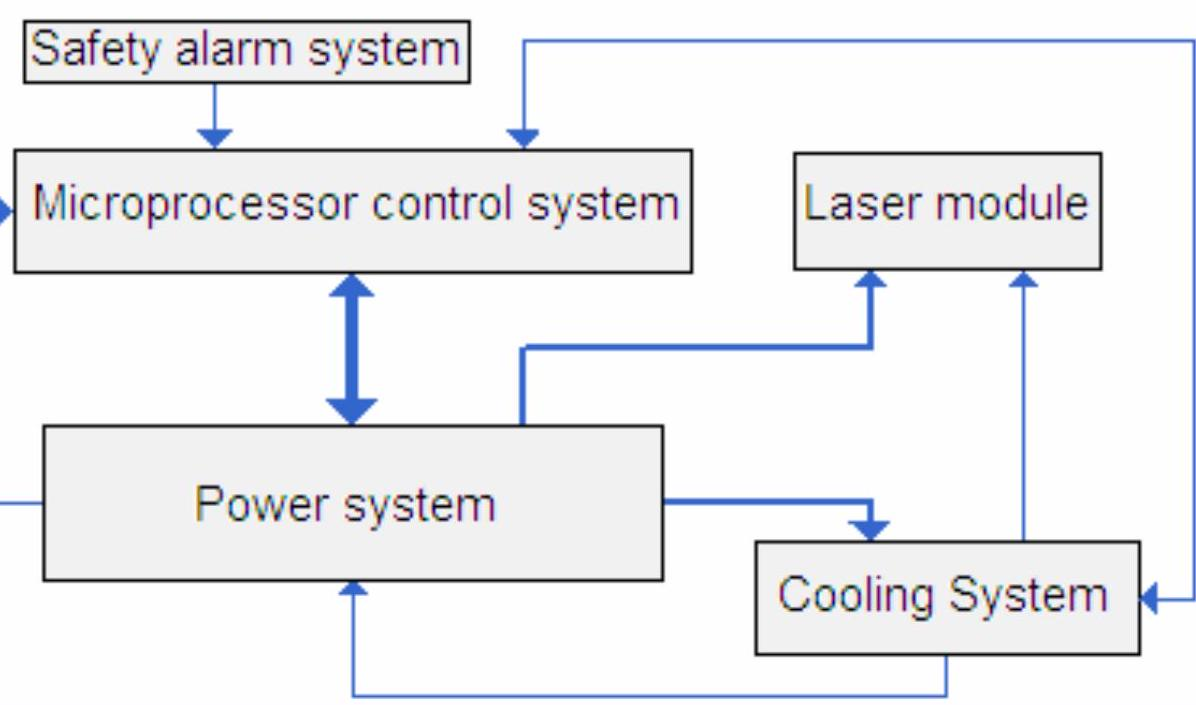
\includegraphics[alt={},max width=\textwidth]{0673f156-6613-4c24-ad16-c1dd5450a875-58_705_1196_1925_358}
\end{center}
\end{figure}

\begin{figure}[h]
\begin{center}
\captionsetup{labelformat=empty}
\caption{Figure 2.2.2 schema a blocchi del sistema di diodo Laser System}
  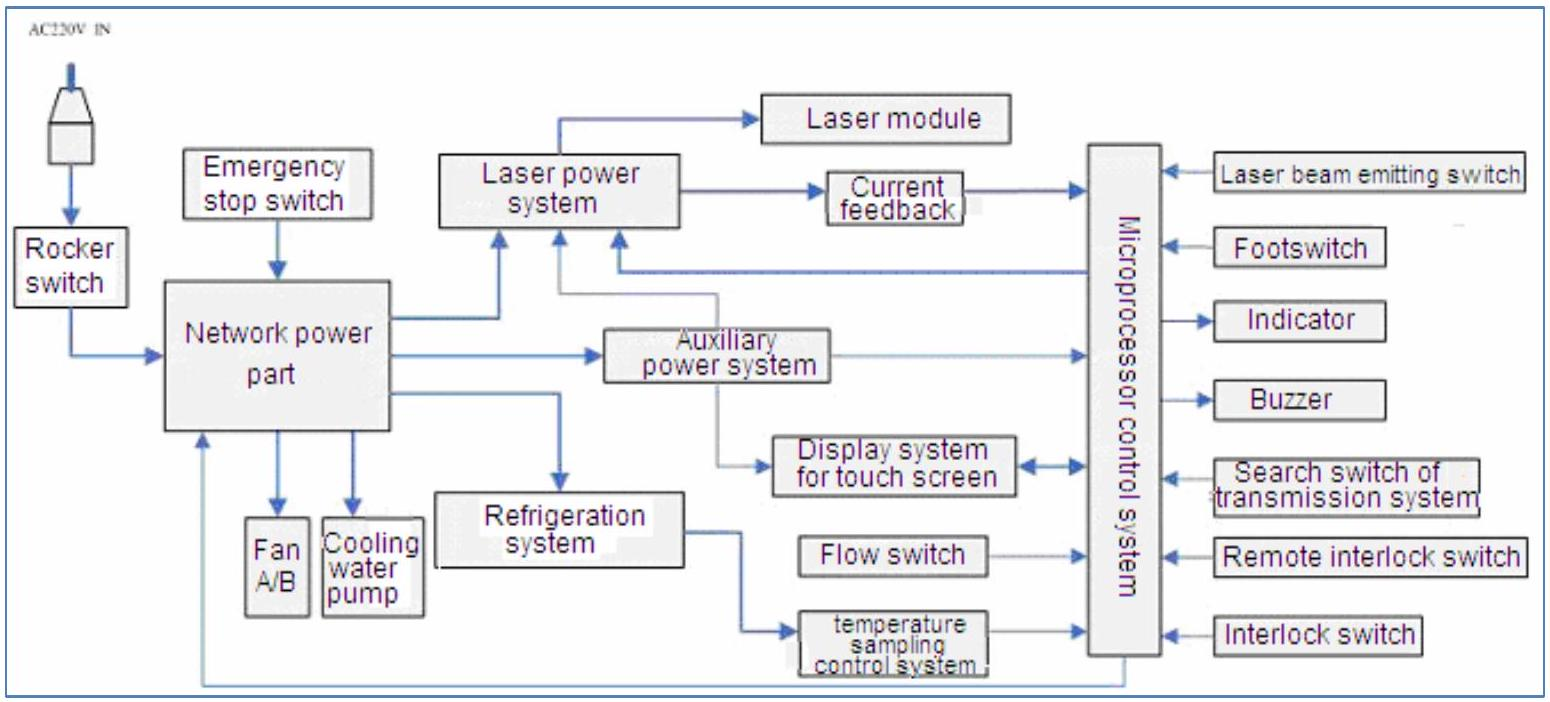
\includegraphics[alt={},max width=\textwidth]{0673f156-6613-4c24-ad16-c1dd5450a875-59_702_1550_587_123}
\end{center}
\end{figure}

\section{Utilizzo:}
CAUTION\\
Tutte le persone che utilizzeranno la macchina devono studiare questo manuale con molta attenzione ed in seguito, prendere le misure di sicurezza necessarie, prima di iniziare una qualsiasi delle procedure. L'utilizzo errato di tale apparecchiatura potrebbe causare gravi danni alla salute del paziente / cliente.

\section{Indicazioni}
Attenzione le indicazioni riportate sono puramente indicative, esse vanno valutate in funzione del trattamento e della persona da trattare qualsiasi impostazione o indicazione va considerata puramente indicativa. L'operatore deve valutare di volta in volta ed in funzione del soggetto da trattare tutti i parametri e valutare le controindicazioni che si possono incontrare con ogni singolo soggetto.

Sono disponibili presso la nostra azienda corsi di formazione ed informazione sul corretto uso del laser, tutti gli utilizzatori si devono, prima dell'utilizzo dell'apparecchiatura, informare sui seguenti argomenti:

\begin{itemize}
  \item Uso dell'apparecchiatura con l'ausilio di un formatore, e del manuale d'uso
  \item Principi di funzionamento degli apparati laser
  \item Uso specifico del modello in dotazione nell'istituto od ambulatorio
  \item Applicazioni e avvertenze sull'uso dell'apparecchiatura
  \item Effetti collaterali
  \item Informazione presso altri istituti e/o conoscenze sul corretto uso dell'apparecchiatura
  \item Studio di tutte le avvertenze.
  \item Informazione sui sistemi di sicurezza da adottare
  \item Cosa si deve fare in caso di anomalia tecnica o di lesioni procurate.
\end{itemize}

L' apparecchiatura laser a diodo 808 è adatto allo sfoltimento pilifero delle persone.\\
Le zone che si possono trattare sono le seguenti:

\begin{itemize}
  \item Viso ad eccezione della zona oculare e del padiglione auricolare\\
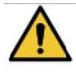
\includegraphics[max width=\textwidth, alt={}, center]{0673f156-6613-4c24-ad16-c1dd5450a875-59_74_76_2547_1165}
  \item Labbra (attenzione ad eventuale trucco permanente)
  \item Barba Maschile
  \item Barba Femminile\\
V/nat
  \item Mento / sottomento
  \item Collo parte superiore
  \item Ascelle
  \item Braccia
  \item Gambe
  \item Cosce
  \item Seno
  \item Zona bikini
  \item Braccia
  \item Avambraccio
  \item Petto
  \item Schiena
  \item Mani
  \item Piedi
\end{itemize}

\section{Controindicazioni}
\begin{itemize}
  \item Gravidanza
  \item Soggetti di minore età (solo se autorizzati da genitori o chi ne fa le veci)
  \item Allattamento
  \item Persone con malattia della pelle o infezioni nelle aree di trattamento
  \item Herpes simplex
  \item Persone che si sono sottoposte ad altri tipi di depilazione IPL, Cera, Ago ecc. dall'ultimo trattamento devono essere trascorsi almeno due mesi, questo per poter valutare al meglio la nuova metodica
  \item Persone affette da psicosi
  \item Disturbi alla coagulazione
  \item Soggetti che assumono sostanze stupefacenti, perché più fotosensibili.
  \item Persone con pelle fotosensibile
  \item Persone con trascorsi di cheloide (tumori cutanei benigni)
  \item Persone che sono allergici ai farmaci idrochinone o altri agenti sbiancanti
  \item Persone con tumore maligno
  \item Pazienti facenti uso di medicinali che vietano l'esposizione ai raggi solari con gamma da 515 a 1200 nm .
  \item Pazienti diabetici
  \item Squilibri ormonali e squilibri mentali
  \item Esposizione al sole negli ultimi 15 gg
  \item Non esporre al sole la zona trattata per almeno 15 gg
  \item Non trattare Nei e Angiomi
  \item Non trattare macchie dovute al sistema epatico
  \item Non trattare macchie cutanee
  \item Non trattare superfici con Tatuaggi
  \item Dermatosi infiammata
  \item Problematiche del sistema immunitario
  \item Persone con assunzione Lsotretinoin negli ultimi 6 mesi (farmaco per acne)
  \item Terapie per la cellulite nelle aree da trattare (attendere alcune settimane dall'ultimo trattamento)
  \item Trascorso di cancro cutaneo o possibili affezioni da tumori maligni
  \item Trattamento di radioterapia o chemioterapia negli ultimi 6 mesi
  \item Regime di steroidi negli ultimi 6 mesi
  \item Medicinali fotosensibilizzanti negli ultimi 3 mesi
  \item Epilessia
  \item In presenza di qualsiasi altra condizione che secondo il medico curante potrebbe rendere insicuro il trattamento
  \item Soggetti minori o affetti da handicap. Chiedere autorizzazione e consenso al genitore o chi ne fa le veci.\\
What
  \item Lenti a Contatto (in questo caso farle togliere)
  \item Operazioni agli occhi
  \item Non esporsi al sole o lampade abbronzanti per almeno 15-20 gg dopo il trattamento
  \item Presenza di protesi sia metalliche che siliconiche o derivati, e fili di trazione dovuti ad interventi di chirurgia estetica in questo caso chiedere sempre consiglio al proprio chirurgo estetico
  \item Disfunzioni ormonali, esse possono incidere sul buon risultato
\end{itemize}

Il sistema non ha alcun effetto significativo sui peli bianchi, allo stesso tempo con persona con la pelle abbronzata il risultato si riduce. Con pelli abbronzate o con pelli scure usare maggior cautela.

\section{Caratteristiche e principio di funzionamento}
Il principio fondamentale di funzionamento del sistema laser a diodo è basato su effetto biologico. Questo prodotto adotta il laser con lunghezza d'onda di 808 nm per irradiazione, che sono particolarmente sensibili ai melanociti di follicolo pilifero senza danneggiare l'epidermide normale. La luce può essere assorbita dalla melanina nel fusto del pelo e follicoli piliferi e viene trasformata in calore, così aumenta la temperatura del follicolo pilifero, quando la temperatura è aumentata in misura maggiore, là viene danneggiato il follicolo pilifero, quindi, i peli danneggiati possono essere rimossi dopo un processo fisiologico naturale, in modo che si possa raggiungere l'obbiettivo prefissato di un diradamento della densità pilifera, attenzione in nessun modo si può definire depilazione permanente.

\section{Effetti clinici}
\section{Sicurezza:}
L'apparecchiatura ha ottime prestazioni, è stata progettata per avere una lunga durata, adotta un microprocessore per il controllo dell'apparecchiatura in tempo reale.

\section{Efficace:}
Le e lunghezze d'onda coprono tutte le tipologie di pelli (standard, chiare e scure) penetrano il derma profondo e sottocutaneo, ciò permette di agire sulle diverse profondità del bulbo pilifero Indolore:\\
Il manipolo e lo zaffiro vengono portati durante il trattamento ad una temperatura a contatto dell'epidermide di circa $0 \sim 4^{\circ} \mathrm{C}$ tale temperatura viene mantenuta costante per tutto il periodo di trattamento, questo per permettere al cliente / paziente di non sentire eccessivo calore e dolore.

Semplice: L'interfaccia uomo-macchina - touch screen, intuitivo è facile da usare, quindi, il suo funzionamento è semplice e veloce.

Depilazione progressiva: Adatto a tutti i tipi di colorazione del pelo e dell'epidermide

\section{Potenziali Rischi}
\begin{itemize}
  \item Le complicanze più comuni per l'utilizzo del sistema laser: eritema ed edema follicolare localizzati, la maggior parte di essi possono scomparire da soli dopo un paio d'ore.
  \item Rare complicanze sono la ticchiolatura locale (efelidi e macchie), rossori, vesciche, pigmentazione o ipopigmentazione ed aumento della secrezione di sebo.
  \item L'insorgenza di reazioni avverse dopo la depilazione laser sono dovute nella maggior quantità dei casi ad un utilizzo elevato dell'energia / potenza / fluenza ad un uso prolungato sulla stessa zona trattata nel medesimo trattamento ed anche ad un contenuto elevato di melanina nella zona trattata.
\end{itemize}

\section*{W $/ \sqrt{6++}$ }
Altre reazioni sono dovute a fattori esterni quali:

\begin{itemize}
  \item Cambiamenti stagionali
  \item Esposizioni solari sia naturali che artificiali
  \item Assunzione di farmaci fotosensibilizzanti
  \item Prodotti non detersi nelle zone trattate quali profumi ecc.
  \item Irritazioni cutanee nella zona trattata (rasatura con lame)
\end{itemize}

In tutti questi casi prestare attenzione ed eventualmente sospendere il trattamento.\\
$\mathrm{E}^{\prime}$ consigliabile eseguire con il cliente una intervista conoscitiva per valutare eventuali contrindicazioni.

\begin{itemize}
  \item Portare a conoscenza il cliente delle avvertenze pre e post trattamento
  \item Valutare le aspettative del cliente
  \item Informarlo sui reali risultati che si possono raggiungere
  \item Far firmare sempre un consenso informato
  \item Si consiglia di effettuare delle foto sulle zone da trattare
\end{itemize}

\section{Metodo di trattamento}
L'apparecchiatura deve essere usata solo ed esclusivamente presso locali e da personale specializzato ed autorizzato aventi i requisiti richiesti. La formazione degli operatori è a carico dell'acquirente.\\
L'importatore, il distributore declinano ogni responsabilità civile e penale, amministrativa per un uso improprio della apparecchiatura.

Le seguenti indicazioni e metodi di trattamento sono da considerare solo di riferimento, i parametri e le procedure di funzionamento sono da valutare in funzione della clientela e vanno adattate ad ogni singolo soggetto. Consapevoli che in determinate operazioni di regolazione si possono raggiungere migliori risultati rispetto a condizioni e regolazioni più basse si deve considerare l'elevato rischio durante il trattamento con conseguenze anche gravi sul cliente / paziente.\\
Si consiglia pertanto l'utilizzo dell'apparecchiatura in modalità e con regolazioni in sicurezza, meglio consigliare alla clientela qualche trattamento in più che incorrere in rischi inutili.

La quantità di trattamenti necessari dipende da diversi fattori, quali:

\begin{itemize}
  \item Fase del pelo
  \item Predisposizioni genetiche
  \item Tipo di pelo
  \item Tipo di pelle FTP
  \item Costanza nei trattamenti e del piano stabilito\\
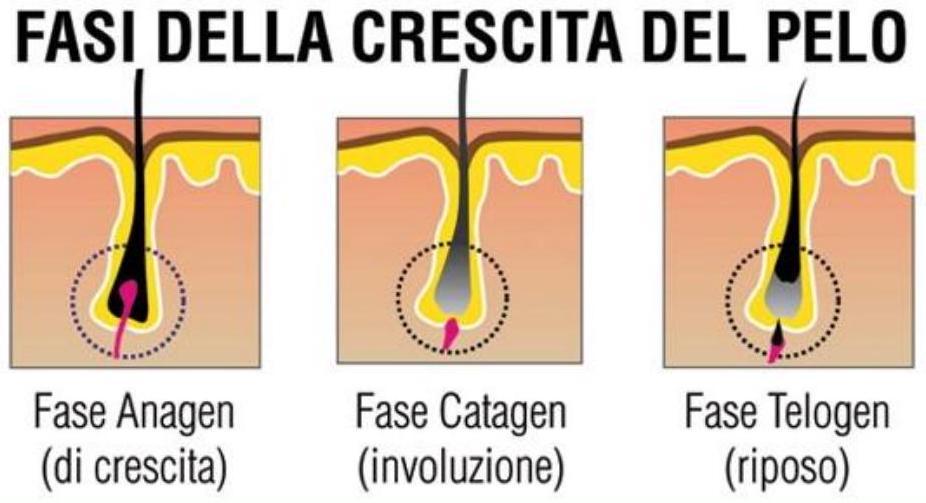
\includegraphics[max width=\textwidth, alt={}, center]{0673f156-6613-4c24-ad16-c1dd5450a875-62_503_926_2122_383}
  \item La Fase Anagen è la fase attiva, durante la quale i peli sono ricchi di melanina e quindi ottimo bersaglio del laser
  \item La Fase Catagen è quella in cui il bulbo si riassorbe e la parte inferiore del follicolo cessa di crescere
\end{itemize}

$$
\sqrt{1} \sqrt{1 a+}
$$

\begin{itemize}
  \item La Fase Telogen è di riposo, in questa fase il follicolo si prepara allo sviluppo di un nuovo pelo.\\
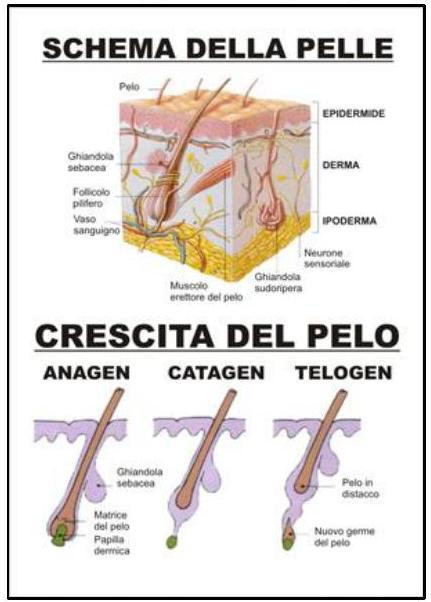
\includegraphics[max width=\textwidth, alt={}, center]{0673f156-6613-4c24-ad16-c1dd5450a875-63_602_431_548_278}\\
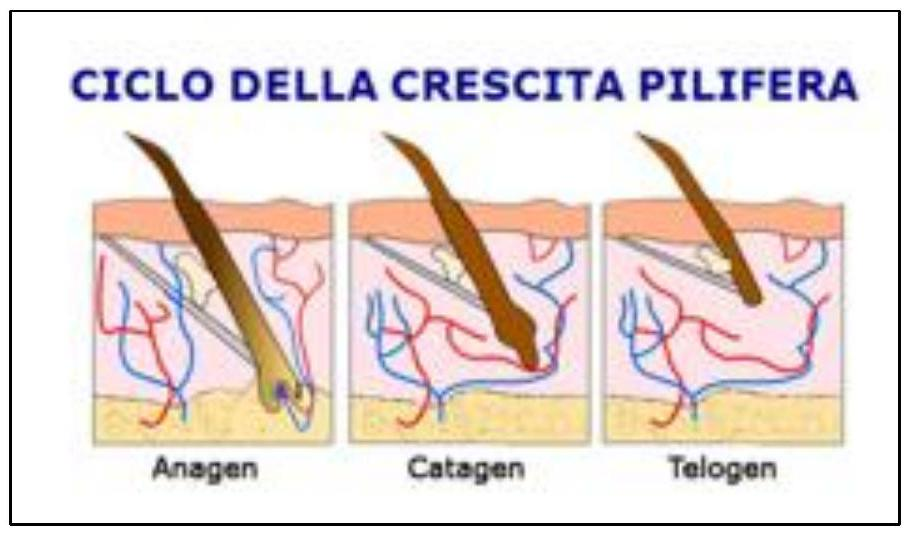
\includegraphics[max width=\textwidth, alt={}, center]{0673f156-6613-4c24-ad16-c1dd5450a875-63_534_908_584_826}
\end{itemize}

\section{Anagen}
A livello del cuoio capelluto, la fase d'attività del follicolo, che prende il nome di anagen, dura normalmente 3-7 anni. I nostri capelli si ricambiano ogni 3-7 anni: quando il capello "vecchio" cade ed è sostituito da un nuovo capello "giovane".\\
A livello di altre regioni del corpo la durata dell'anagen è molto più breve: ad esempio 1-6 mesi per le ciglia, 20-40 giorni per la peluria delle braccia o delle gambe.

\section{Catagen}
È una fase di transizione molto breve che dura circa $3-4$ settimane. In questa fase la matrice del pelo interrompe la sua attività e il follicolo inizia a risalire verso la porzione più superficiale della cute, dove trascorrerà la sua fase di riposo (Telogen).

\section{Telogen}
Finita la fase di crescita, il follicolo entra in riposo (Telogen) e interrompe la sua attività produttiva per circa 3 mesi. Durante il Telogen la matrice del pelo è scomparsa e il follicolo interrompe ogni attività, il pelo però non cade ma rimane ancorato al follicolo.

\section{Preparazione}
Prima di iniziare la serie di trattamenti su di un cliente eseguire un'attenta valutazione sulle caratteristiche di fototipo, del tipo di pelo, valutare le possibili controindicazioni ed esporle al cliente / paziente, eseguire un'intervista conoscitiva del cliente / paziente effettuare un precorso della durata e della quantità di trattamenti da eseguire e far firmare privacy e consenso informato al cliente.

Preparare la zona procedendo con una pulizia e detersione della zona e con la rasatura dei peli con apparati elettrici quali regola barba, l'utilizzo di rasoi a lama può causare irritazione della pelle nel caso di loro utilizzo è consigliabile procedere alla rasatura almeno due giorni prima.\\
Procedura

\section{La procedura qui indicata è da considerarsi indicativa, essa può subire variazioni e deve essere adeguata ad ogni singolo cliente}
Eseguire un'intervista conoscitiva del cliente portandolo a conoscenza delle controindicazioni e dei risultati che si possono ottenere con il trattamento.\\
Far compilare il consenso informato, in caso di dubbi sul trattamento o di patologie chiedere sempre informazioni tecniche o mediche al medico curante del cliente; rispettare sempre, le leggi vigenti del proprio territorio, esse andranno personalizzate dall'acquirente in base alle sue esigenze.

\section*{W $/ \sqrt{6+}$ }
\begin{itemize}
  \item L'operatore ed il cliente devono obbligatoriamente indossare occhiali di protezione forniti nella dotazione dell’apparecchiatura, allo scopo di impedire danni all’apparato oculare.
  \item Detergere e pulire la zona da trattare da prodotti cosmetici, profumi, deodoranti o trucco.
  \item Proteggere i nei, macchie cutanee o trucco permanente e tatuaggi con matita bianca, cotone bianco o con apposite coperture.
  \item Stendere un leggero velo di gel trasparente sulla zona da trattare, ciò permette di ridurre il calore nella zona trattata diminuendo la sensazione di dolore, inoltre il gel permette (Cristal) di individuare in modo più efficace le zone ove si è già intervenuti.
  \item Proteggere il manipolo con un film trasparente, ciò permette una più facile pulizia del manipolo stesso a fine trattamento oltre che impedire eventuali trasmissioni di infezioni cutanee da un cliente ad un altro (disinfettare comunque sempre il manipolo tra i diversi clienti e mantenerlo pulito ed asciutto).
  \item Impostare i parametri di trattamento in funzione della tipologia del cliente
  \item Nel caso dei baffetti inserire tra il labbro ed i denti un tubolare di cotone o garza leggermente imbevuta di acqua, questa metodica non permette alle piccole radiazioni di raggiungere i denti eliminando eventuali sensazioni di dolore
  \item Effettuare sempre un test di prova sulla zona partendo da parametri molto bassi, solo a test positivo procedere con il trattamento.
  \item Personalizzare i parametri per ogni singolo cliente.
  \item Stabilire con il cliente un programma per la serie di trattamenti.
  \item Posizionare la testina emettitore del manipolo sulla zona da trattare premendo leggermente in modo da rendere praticamente ermetica la zona sottostante l'emettitore.
\end{itemize}

\begin{figure}[h]
\begin{center}
  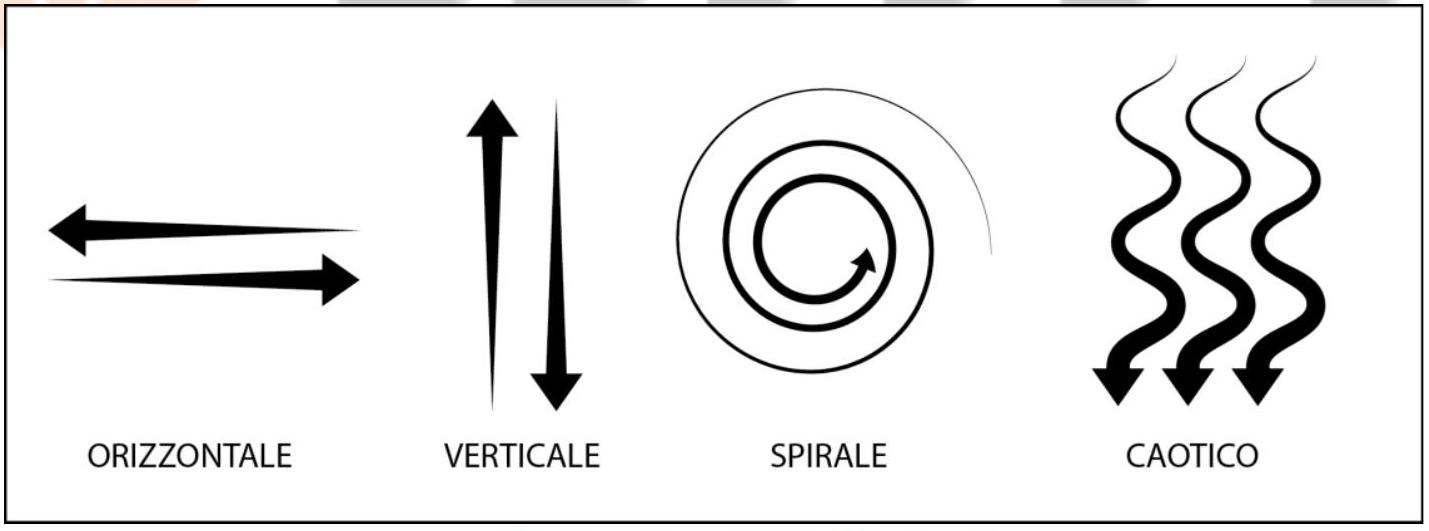
\includegraphics[alt={},max width=\textwidth]{0673f156-6613-4c24-ad16-c1dd5450a875-64_531_1429_1779_246}
\captionsetup{labelformat=empty}
\caption{Movimenti possibili del Manipolo Laser}
\end{center}
\end{figure}

Tutte le indicazioni dei parametri e delle regolazioni riportate sul manuale d'uso devono essere valutate in funzione del tipo di trattamento e del cliente/paziente dopo attento esame di valutazione.

\section{Impostazione Parametri:}
\begin{itemize}
  \item Impostare i parametri di riferimento ed effettuare delle prove sulla zona da trattare, è sconsigliato effettuare prove in zone visibili, quali il viso. Il parametro indicativo per un buon risultato è la sensazione da parte del cliente di piccole punture in corrispondenza del pelo, se ciò non avviene può essere elevata la densità di energia oppure è sintomo di scarsa o nulla densità pilifera.\\
Whate
  \item Mantenere una adeguata pressione del manipolo sulla pelle, una pressione troppo elevata può impedire nella zona una scarsa irrorazione sanguigna.
  \item Allo scopo di ottenere un valido raffreddamento della zona è consigliato mantenere il manipolo a contatto della pelle per almeno $0,25 \sim 0,50$ secondi prima di premere il pulsante dell'emissione.
  \item Muovere il manipolo con movimenti lineari o a spirale in funzione della zona: zone piccole esempio baffetti con spot singoli e lineari, zona braccia con movimenti lineari, zona schiena con movimenti lineari o a spirale. Adeguare sempre la velocità di movimento alle frequenze di lavoro impostate ed alla potenza scelta.
  \item Non passare più di due volte sulla stessa zona, con alcune regolazioni ed impostazioni si possono raggiungere anche le quattro volte, adeguarsi sempre ai corsi di formazione che la stessa azienda mette a disposizione.
  \item I risultati ottenuti possono variare in funzione dei soggetti o delle zone trattate, ricordarsi che molti fattori possono influire sull'efficacia dei risultati, tra essi bisogna considerare anche la naturale crescita fisiologica del pelo (la maggior efficacia è colpire il pelo ed il bulbo nel loro periodo anagen) oltre la considerazione che, in ogni parte del corpo la crescita del pelo e la sua vita cambia da zona a zona, è consigliabile per le zone del viso ascelle ed inguine periodi di intervallo tra i vari trattamenti di un mese , per le zone del tronco si può arrivare anche ad intervalli di due mesi .
  \item A fine trattamento, trattare la zona con prodotti lenitivi e/o idratanti.
\end{itemize}

\section{Variabili dei parametri}
\begin{itemize}
  \item Con bulbo pilifero profondo impostare la durata dell'impulso "lunga".
  \item Con bulbo pilifero meno profondo impostare durata dell'impulso "corta".
  \item Con pelo grosso impulso "lungo e fluenza bassa".
  \item Con pelo sottile durata impulso "breve e la fluenza alta".
  \item Con densità pilifera alta, "fluenza bassa".
  \item Con densità pilifera bassa, "fluenza alta".
  \item Con pelo scuro la durata impulso "lunga e la fluenza bassa".
  \item Con pelli chiare durata impulso "corta e fluenza alta".
  \item Con pelli scure "fluenza bassa".
  \item Con pelli scure tempo di lavoro basso
\end{itemize}

\section{Attenzione:}
Tutte le indicazioni riportate devono essere valutate di volta in volta ed impostate in base alle esigenze, considerando le caratteristiche di ogni singolo cliente / paziente ricordando che anche lo stesso cliente nel corso del periodo di trattamento subisce variazioni come ad esempio: densità pilifera, fototipo, condizioni fisiche, ecc. La stessa apparecchiatura (MANIPOLO) con l'uso ha un deterioramento nella fluenza in funzione della quantità di spot eseguiti.\\
Sottoporre il manipolo a controlli periodici con apposito strumento, lo stesso conta impulsi dell’apparecchiatura, può essere un valido indicatore.


\end{document}